\documentclass[conference,compsoc,a4paper]{IEEEtran}
\usepackage{geometry}
 \geometry{
 a4paper,
 total={170mm,257mm},
 left=20mm,
 top=20mm,
 }

\usepackage[backend=bibtex]{biblatex}
\usepackage{array}
\usepackage[utf8]{inputenc}   % <<<<< Linux
\usepackage[nomain,acronym,xindy,toc]{glossaries} 
\usepackage{graphicx}
\usepackage{tabularx} 
\usepackage{float}

\usepackage{color, colortbl}
\definecolor{Gray}{gray}{0.9}
%Includes "References" in the table of contents
%\usepackage[nottoc]{tocbibind}

\bibliography{references} % or

\hyphenation{op-tical net-works semi-conduc-tor}
\loadglsentries[main]{xacronyms}

\newcolumntype{Y}{>{\centering\arraybackslash}X}
\newcolumntype{M}[1]{>{\centering\arraybackslash}m{\linewidth/#1}}

\begin{document}


\title{Hyper-linked Communications: WebRTC enabled asynchronous collaboration}

\author{\IEEEauthorblockN{Henrique Rocha}
\IEEEauthorblockA{Instituto Superior T\'{e}cnico\\}
\IEEEauthorblockN{Av. Prof. Dr. Anibal Cavaco Silva\\
2744-016 Porto Salvo, Portugal\\
henrique.rocha@tecnico.ulisboa.pt}}

\maketitle

\begin{abstract}
The Hyper-linked communications concept applies much of the hypermedia concepts, widely used on Web content. This paradigm allows to synchronize, structure and navigate communication content integrated into voice and video calls.

Voice and image together can express emotions like no other medium can. With hypermedia concepts, we can add more value to conference calls.

\emph{WebRTC} technology allows real time communications between web browsers without the need to install additional software. The nature of web browser applications already follows the hypermedia concept, which makes \emph{WebRTC} the ideal technology to apply the hyper-linked communications concepts.
The web browser platform provides an abstraction layer that makes it possible to create applications that run independently from the operating system.
The native support for \emph{WebRTC} in operating systems extends its usage to outside the web browser, allowing for the exploration of functionalities for which web browsers provide poor support, such as video recording and massive information storage.

Our goal was the development of an application targeted to the web platform, resorting to \emph{WebRTC}, that leveraged the hyper-linked communications by providing a conference environment enriched with multiple media types, collaborative text editors, time annotations, instant messaging and a mechanism to superimpose hyper-content to video.
\end{abstract}

\IEEEpeerreviewmaketitle

\section{Introduction}
\label{chapter:introduction}

\subsection{Background}
\label{section:background}

	As communications technologies appeared, we adapted the way we communicate. The purpose of this project is not the replacement of the current video and audio communications, but to enrich them with hyper-media content and make them a more natural and easy to learn process. 

	With the advent of WebRTC and its successive integration with web browsers, it became possible to develop video conference web applications without plugins, this presents a range of possibilities on what can be implemented using already existing web technologies.
		
    Furthermore, real time communication applications can make a significant difference on business, education and health sectors by providing tools for developing teaching and learning online, teamworking and socializing web applications.

\subsection{Proposed Solution}
\label{section:proposed}

	Our goal in this project is to develop an application targeted to the web platform, resorting to \gls{WebRTC}, that leverages the hyper-linked communications by providing a video conference environment enriched with interactive and non-interactive discrete media types such as images, subtitles, forms and all types of content that can be added using \gls{HTML}5, \gls{CSS}3 and \emph{JavaScript} including continuous media types such as video, music and animations.

	One of the key features of this project is the ability to navigate in time in order to reproduce the conversation again or introduce hyper-content to it such as time annotations, interactive lists of topics and subtitles. In this context we also provide a simpler method for creating and synchronizing hyper-content using \gls{QR} codes.

	In addition to this conference environment, which provides different functionalities than traditional conference environments such as \emph{Skype} and \emph{Google Hangouts}, we also enable a collaborative text editor and a chat that supports sending time hyper-links and files to conference participants.

	Furthermore, another relevant feature is the possibility to compose multiple video streams into a single one, which enables adding more users to conference rooms without impacting on clients performance. Users can change to individual streams on demand or automatically to the talking users.
        

\subsection{Thesis Contribution}
\label{section:contribution}

Making it clear, this project aims to complement current audio, text and video communications in order to create rich and collaborative interfaces with the ability to add more content on a future time (\emph{e.g.} creating time annotations for improving content search) in order to increase its value. It is also important to highlight another goal of this project which is the ability to navigate in time by rewinding communications, fast-forward and jump to certain points.

	We have presented an architecture that can meet our goals, implemented the respective prototype and tested it with real users and performance benchmarks.

	According to Martin Geddes, the quality of the interaction worsens as the number of users increase\cite{geddes}. In our testing phases we will quantify and qualify the impact of increasing users on the interface and performance of our prototype. 

	All the problems faced during the development and limitations were reported on the thesis so that a future project better then ours can be easily and better developed.

\subsection{Outline}

This rest of this document is structured as follows:

\begin{itemize}

\item \textbf{Chapter \ref{chapter:relatedwork}} describes the previous work in the field.
\item \textbf{Chapter \ref{chapter:architecture}} describes the system requirements and the architecture for an Web Application that fulfills the goals of this thesis.
\item \textbf{Chapter \ref{chapter:implementation}} describes the implementation of our Web Application and the technologies chosen.
\item \textbf{Chapter \ref{chapter:evaluation}} presents the evaluation tests performed and the corresponding results.
\item \textbf{Chapter \ref{chapter:conclusion}} summarizes the work developed and proposes future work.
\end{itemize}

\section{Related Work}
\label{chapter:relatedwork}

One way to overcome the \gls{IPv4} address scarcity problem \cite{ipv4} was the development of a mechanism that groups multiple address into a single one, the machine that is assigned that address is then responsible for redirecting messages to members of its group using their private addresses, each connection in the private network is identified publicly by the same \gls{IP} address with a different port. This technique is known as \gls{NAT}\cite{rfc3489}.

\gls{NAT}s weaknesses are being exposing at the application layer, namely impacting applications that require direct communications between two private networks.

In order to implement an hyper-linked communication solution, several design decisions had to be made. The limitations imposed by the \emph{Internet's} structure, its protocols and a browser's capabilities are key factors to consider when implementing a solution that allows bi-directional communications, interactive media and collaboration environment.

Due to the use of \gls{NAT}, bi-directional communications between clients have different needs from request-response based communications between clients and servers.
This lead to the appearance of mechanisms such as \gls{STUN}, \gls{TURN} and \gls{ICE}, in order to bypass the limits imposed by \gls{NAT}.

\gls{STUN}, \gls{TURN} and \gls{ICE} \cite{natvoip} servers are a possible solution to overcome \gls{NAT}'s exposed weaknesses to applications that require communications between two private networks. 


When connection is established, \gls{WebRTC} came to simplify how audio and video are transmitted through web browsers. \gls{WebRTC} is an open source technology that defines a collection of standard protocols and \emph{JavaScript} \gls{API}s for web browser based real time communications without installing any additional application or plug-in. 

\gls{WebRTC} uses \gls{SDP} \cite{rfc4566} to define peer connection properties such as types of supported media, \emph{codecs}, protocols used and network information. An \gls{SDP} offer describes to other peers the expected type of communication and its details, such as used transport protocols, codecs, security and other.


Some operating systems such as \emph{Android}, \emph{iOS}, \emph{Linux}, \emph{OSX} and \emph{Windows} implement native \gls{WebRTC} libraries, extending the usage of \gls{WebRTC} to applications outside the web browser. This native support can help to implement applications that record video and audio streams for further playback.

However, \gls{WebRTC} by itself does not define how users get to know each other nor how information flows between users. For this reason, we have studied the multiple ways we could implement this \emph{get-to-know} mechanism which is known as signaling protocol.


  Signaling is the process by which applications exchange connection information about peers and servers, their capabilities and meta-data.
  In particular, \gls{WebRTC} does not implement signaling, as different applications may require different protocols and there is no single answer that fits all problems.
  As a consequence, multiple options are available for filling the missing \gls{WebRTC}'s signaling component, which can be performed using \gls{SIP}\cite{rfc3261}, \gls{XMPP}, \emph{WebSockets}, \emph{Socket.io}\footnote{\url{http://socket.io/}(accessed June 1, 2015).}, \gls{SigOfly}\cite{sigofly} or by implementing a custom protocol.

  One of \gls{WebRTC} signaling's requisites is bi-directional communication. The \emph{WebSocket} protocol allows bi-directional communications over a full-duplex socket channel \cite{rfc6455}, by other words it supports sending and receiving data simultaneously.

With the communications establishment issue solved, we had to discuss the different types of media and what can be done with each kind in order to increase the value of communications among users. In this context, we have studied solutions and libraries that allow us to implement our prototype with time manipulation features, collaborative text edition, record and playback interactive video. 

	\emph{Hypermedia} concept brings the possibility to organize and overlay multimedia elements into a nonlinear linear structure holding the promise of future technology and features. Languages such as \gls{SMIL}~\cite{hyval}, \emph{HyVAL}~\cite{hyval} and \gls{HTML} can be used to implement the \emph{Hypermedia} concept. Two examples of applications that captured our attention were \emph{HyperCafe}~\cite{hypercafe} and \emph{Hyper-Hitchcock}~\cite{hitchcock} which explored interactive video features.

  Using technologies that relies only on web standards, like \gls{CSS}, \gls{HTML}5, \emph{JavaScript} and \gls{SVG}, will make possible to develop an application that applies the hypermedia concept with the advantage of being compatible with a greater amount of web browsers.
  
\subsection{Extending collaboration tools with time manipulation}
\label{collab}

Real time collaboration applications have become a huge help on team tasks, providing a great boost on business, research and investigation velocity.

 Our first concern on real time collaboration applications is the data storage and representation. Storing multimedia content on a web client is not a viable solution because the local storage is limited to at most five megabytes per origin. Additional servers will be required to process and record the large amount of data generated by audio and video streaming.
 
\gls{KMS} supports streaming over \emph{WebRTC}. Another important component of \gls{KMS} is \emph{Kurento Repository}, which supports recording and playing directly from \emph{MongoDB}. That is important for providing a scalable media storage. 
	
     \gls{OT} technology was originally developed for consistency maintenance and concurrency control over distributed objects.
     \gls{OT} algorithms are mainly used in collaborative applications such as distributed document edition.

	Among mutiple \gls{OT} platforms and libraries we present \emph{ShareJS}\footnote{\url{http://sharejs.org/}(accessed June 2, 2015).}, \emph{TogetherJS}\footnote{\url{http://togetherjs.com/}(accessed June 2, 2015).}, \emph{Goodow}\footnote{\url{http://realtimeplayground.goodow.com/}(accessed June 2, 2015).}, \emph{Etherpad Lite}\footnote{\url{https://github.com/ether/etherpad-lite}(Accessed 20 March 2016)} and \emph{otJS}\footnote{\url{http://operational-transformation.github.io}(accessed March 10, 2016)}.


	\emph{otJS} is a \emph{JavaScript} library that only implements operation transformations over plain text on the client side and requires implementing the content's persistent storage. Besides this drawback, this library is very flexible because it is not tied to a specific database or server side technology.
        


\section{Architecture}
\label{chapter:architecture}

Taking into account the goals of this project and all the technology presented so far. Our proposal is the development of a web application that provides communication and collaboration features in real time.

\subsection{Requirements}
In a general way our system's goal is to provide a multi-party video and audio conference environment that supports chat, time manipulation, collaborative text edition and hyper-content creation.

%RP isto pode ser muito expandido. Podes começar por descrever os goals (mais alto nível): audio e video conferência multi-party, possibilidade de rever o que foi dito antes, chat, etc etc.
% Só depois traduzes isso em requisitos, tanto funcionais como não funcionais
% Depois apresentas a arquitectura, fazendo um paralelo entre os módulo e escolhas realizadas e quais os requisitos que cada um deles satisfaz. 

For our system, our application must provide: a simple way to send instant text messages to the conference participants, ability to recording and playback recorded video including all the hyper-content displayed at that time, mixing multiple user streams into a single stream, create annotations associated to a specified time, allow users to superimpose hyper-content to video given a range of time, search every objects related to a conference room such as hyper-content, time annotations and users, share files and time links among users, sound detection for showing the current speaker, provide a collaborative text edition tool, interpret \gls{QR} codes in order to ease content creation and support database replication.
%RP capacidade de lidar com NAT

	Moreover we allow clients to discover chat rooms and other clients by navigating on the web pages provided by our web server. In addition users can create rooms for multi-party audio and video communication communication which is achieved by using \gls{WebRTC}'s \emph{PeerConnection}.
        %RP falas em peerconnection, mas na figura 3.1 apenas há um cliente, o que obviamente impede mostrar a comunicação entre peers.
        %RP acho que podes fazer outro diagrama com a comunicação entre os vários componentes, onde apareceriam vários clientes. A aí indicas o tipo de ligação entre cada par de componentes (HTTP, PeerConnectino, websocket, MediaStream ...)
        
\subsection{Modules}
In this section we present the several modules that were designed in order com fulfill the set requirements.
	Figure~\ref{fig:modules} presents the structure of our system which was divided into six modules:


\begin{figure}
	\centering
	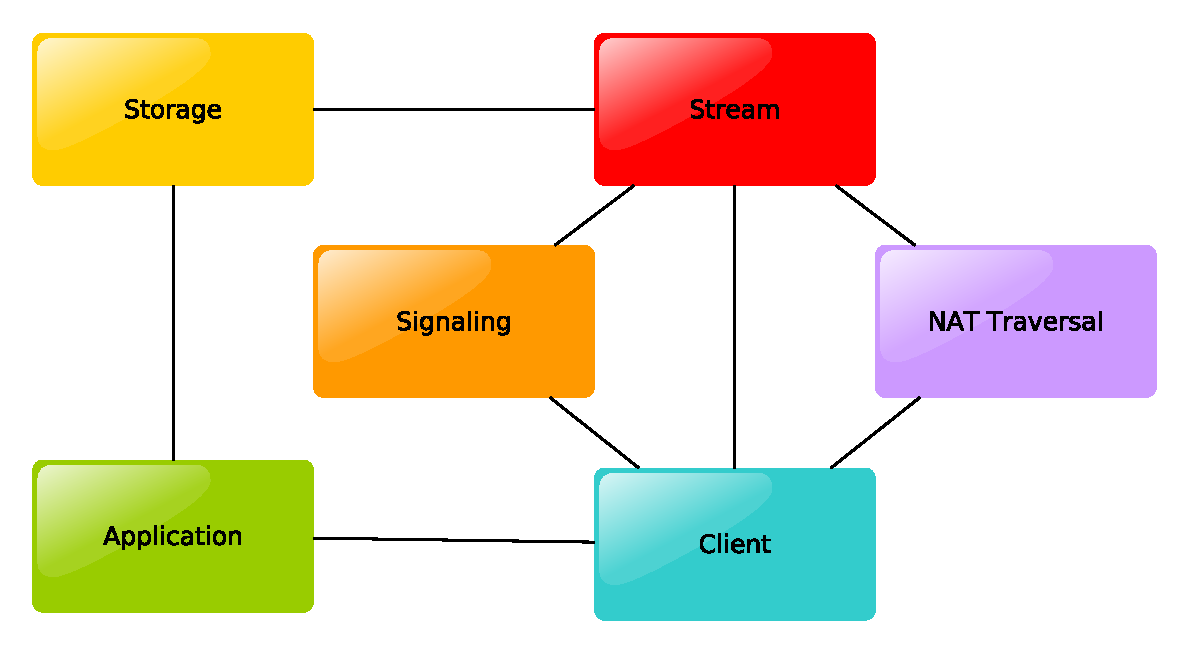
\includegraphics[width=\linewidth]{figures/modules.pdf}
	\caption{System Modules}
    \label{fig:modules}
\end{figure}



\begin{itemize}

\item \textbf{Application module} - responsible for providing information about the relevant modules (\emph{NAT Traversal} and \emph{Signaling}) and user interface to the \emph{Client} in the form of web pages in \gls{HTML} and \emph{JavaScript} libraries through \gls{HTTP}.
 
\item \textbf{Signaling module} - responsible for \emph{Client} and \emph{Stream} coordination which will be performed using \emph{WebSockets}.

 \item \textbf{NAT Traversal module} - \gls{STUN} and \gls{TURN} techniques used by \emph{Client} and \emph{Stream} modules during the \emph{Signaling} phase which ends by establishing the connection between them.

 \item \textbf{Stream module} - responsible to deliver and receive multimedia content from the \emph{Client} using \gls{WebRTC}. 

 \item \textbf{Storage module} - provides two main functionalities: store the model information and media recorded. This is the single module responsible for persistent storage. It stores user and communication data as well as all the data required among user sessions. It is also use to store all the communication streams, so that they can be viewed later.

 \item \textbf{Client module} - responsible for the interaction with the user.

\end{itemize}

%RP Acho que podes escrever muito mais sobre cada componente. Isto está muito curto. Fala de algumas das funções que proporcionam. Vê o que fiz com o Storage Module

%RP também podes fazer um diagrama com vários utilizadores e mostrar quais os streams que vão de e para cada um (mostrar a mistura de som, video, etc).

 
\subsection{Implementation Proposal}
The infrastructure is composed by: web server, stream server, signaling server, database and video repository.
%RP tens da fazer o paralelo entre isto e os componentes apresentados na secção anterior. O mesmo com a imagem, que parece não estar relacionada. Podes colocar os elementos na mesma posição, ou dentro das caixas da imagem 3.1

\begin{figure}[H]
	\centering
	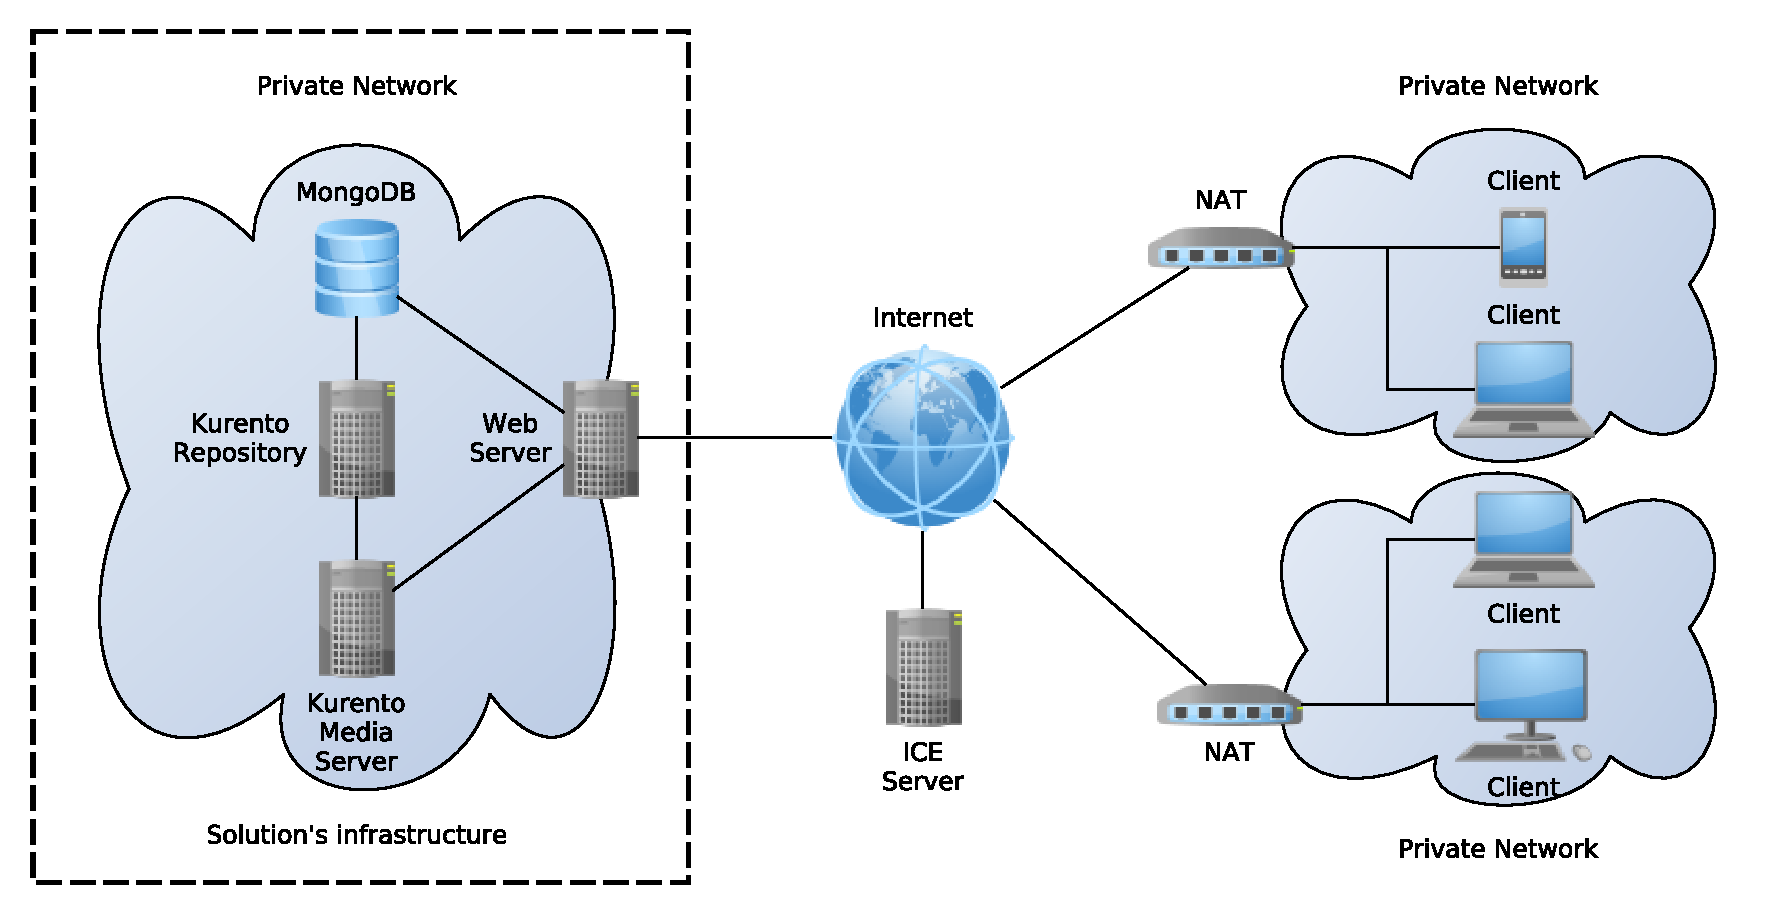
\includegraphics[width=\linewidth]{figures/infrastructure.pdf}
	\caption{System Infrastructure}
\end{figure}

In order to simplify our solution, we propose that the \emph{Application}, \emph{Signaling}, \emph{Stream} and \emph{Storage} modules be implemented within the same server application, so it could be easy to deploy as a single image. To this set of modules, we often call \emph{backend}.

	\subsubsection{Security and authorization}

Having established that the \emph{backend} modules are placed in the same machine, that helps controlling which resources the client has permission to access as those modules are seen as a private network.
%RP na mesma ``server application'' ou ``machine''? São coisa diferentes! Apresentas vantages de instalar tudo na mesma máquina mas não falas das desvantagens. Menor escalabilidade parece-me ser logo uma delas. Na figura 3.2 aparecem várias máquinas!

To qualify the above we provide public access to \gls{HTTP} server ports, maintaining the access to other components restricted through firewall rules.
%RP qualify?
%RP Imagem com firewall e estes portos? Mas isto já me parece muito detalhe de implementação.
In relation to the database there is no directly access from the outside. All the database information is accessed via our application server which validates the permissions of users on our system.

On the other hand, the access to our streaming servers is also restricted, but clients can connect to them after concluding the signaling phase. This signaling phase may or not proceed in function of the client access permissions. For example, if a user is trying to access a private conference room that he is not a member of nor has an invitation link for, the signaling server refuses to start the signaling phase and the user cannot access the streaming server.

The placement of our streaming servers inside a \gls{NAT} also has an important role with respect to external misuse prevention. Otherwise, placing our streaming servers could allow external clients to perform their own signaling protocol and, as a consequence, use our infrastructure without our consent.

\subsubsection{Client connections}
	Although the delegation of processing work to clients can improve our system's scalability, we are concerned about using the least resources possible on the client side, as huge resource consumption may drain battery very fast or may even be impossible to run on mobile devices. We are aware that streaming video from clients is already a very intensive task which we cannot avoid but can improve by delegating the most intensive tasks to our servers. 


	In this context, with a centralized approach, each client must only have one \emph{PeerConnection} to our streaming server and content shown to them is changed on demand either being it an individual or a composite view. Otherwise clients could follow a peer-to-peer connection which would result on maintaining more connections and performing the composition of videos on client side.

	The composition of streams on client side is performed by receiving streams with the best quality possible but, due to undersizing the video of clients into a smaller region, this would result on wasting bandwidth on a quality that is not needed.

	Although the peer-to-peer approach could be used on our system, we conclude that we need to record the video on our streaming server because web clients have a very limited storage and peer disconnections may result on recorded video loss. 

	The same can be concluded to instant message delivery, each client must have only one \emph{WebSocket} connection to the application server which consequently relays the messages to other users.

	Relaying instant messages from clients through the our web servers is easier if all clients are connected to the same server because all messages can be directly delivered without sending messages across multiple web servers. 

	In the context of this thesis, we will not implement sending messages across web servers but, in order to allow our system to scale, we will consider that all conference participants are connected to the same server and our system is scaled by having conference rooms distributed across different servers.

\subsubsection{Software choices}

Furthermore, we have taken into account the compatibility between the streaming server, database and the operation transformation solutions, in order choose the appropriate framework to implement our web server.
%RP esta secção devia começar aqui, a explicar a escolha das tecnologias/produtos a usar em cada componente. O que tens antes são pormenores que só faz sentido discutir no final. Tens de ir sempre do mais geral para o mais detalhado.

We have decided that our solution must use \gls{KMS}. Our web server could be implemented easily with \emph{NodeJS} or \emph{Java} due to the fact \gls{KMS} provides clients for both technologies. But others could also be used as \gls{KMS} also exposes their \gls{API} via \emph{WebSockets}.

Due to the fact we are going to use \gls{KMS} as streaming server solution, we could choose \emph{NodeJS} or any \emph{Java} based web framework for implementing our web application server. We have decided to implement our web server with the \emph{PlayFramework}\footnote{\url{https://www.playframework.com/}(acessed March 25, 2016)} using \emph{Java} because of our previous experience with it.

By default, \emph{Kurento Repository} is implemented over \emph{MongoDB}, for convenience our storage model will also use the same database.

Importantly, for the collaborative text editor, we have chosen \emph{OT.js} due to its server and storage implementation choice independence.

For the \emph{NAT Traversal} module a public \gls{STUN} server can be used for testing our solution. Nevertheless, we recognize that for a production environment we would need to maintain our own \gls{TURN} servers in order to ensure connectivity to all clients.

Not less important, on the client computers, both \emph{Mozilla Firefox} and \emph{Google Chrome} could be installed as web browsers. As such, both should be supported. Libraries such as \emph{jQuery}, \emph{Bootstrap}, \emph{Adapter.js}, \emph{OT.js} can be downloaded from the web server and executed on the client side using any of these two browsers.
%RP relembrar que o IE e o Safari não suportam webrtc?

\begin{table}[H]
\centering
	\caption{Application Architecture}
	\label{table:apparch}

\resizebox{\columnwidth}{!}{%
    \begin{tabular}{cccccccc@{}m{0pt}@{}}
	\hline 
	\multicolumn{8}{|c|}{\cellcolor{Gray}Application}  &\\[12pt]\cline{1-5}\cline{7-7}
	\multicolumn{1}{|c|}{jQuery} & \multicolumn{1}{c|}{HTML5} & \multicolumn{1}{c|}{CSS3 (Bootstrap)} & \multicolumn{1}{c|}{Signaling} & \multicolumn{1}{c|}{ot.js} & \multicolumn{1}{c|}{\cellcolor{Gray}} & \multicolumn{1}{c|}{adapter.js} & \multicolumn{1}{c|}{\cellcolor{Gray}} &\\[12pt]\hline
	\multicolumn{1}{|c|}{HTTP} & \multicolumn{2}{c|}{User Interface}  & \multicolumn{3}{c|}{WebSocket}    & \multicolumn{2}{c|}{WebRTC}      &\\[12pt]\hline
	\end{tabular}
}
\end{table}

%RP acho interessante o que queres fazer aqui mas acho que está mal conseguido. A linha de baixo, devia ter coisas ao mesmo nível, o que não aconteçe.
% Qual a razão para HTTP estar por baixo do jquery e user interface estar ao lado?
% Sugiro colocar a applicação no meio e as várias interfaces (webrtc, websocket e http) uma de cada lado (esquerda, baixo e direita), indicando o que fica do outro lado (outro cliente, servidor web, servidor stream, etc)

Table~\ref{table:apparch} presents the application architecture and the underlying technologies seen from the user's perspective. \emph{Adapter.js} and \emph{jQuery} will ensure that our application is compatible with the most popular web browsers.
\emph{Bootstrap} will be used to make the user interface more appellative and responsive. With \emph{Bootstrap} it is quite easy to develop applications that adapt to mobile devices with different screen sizes.
%RP bootstrap não aparece na figura!

With respect to displaying content, the synchronization between multimedia elements will be performed through chains of \emph{JavasSript} events or by specifying the interval of time which time content must be visible. Other animations can be implemented with \gls{SVG} embedded on \gls{HTML}.
%RP Caiu do céu! Tens de explicar e ligar melhor a sequencia de texto

\section{Implementation}
\label{chapter:implementation}
\subsection{Data Model}

The data model is a critical component of our solution, as a badly designed model can imply serious difficulties when implementing new features that are not part of the plans. During the course of this project, we had to redesign the model more than once in order to support new features.

In order to offer all the functionalities that we promise, some information about objects must be persistent such as users, groups,relations among users, group memberships, messages, hyper-content, recordings and collaborative editor state. For designing our model we have taken into account generic programming techniques. We observed that operations like searching for an object were quite repeated across different types of objects. 

\subsection{Signaling Protocol}


Although we have mentioned that the signaling protocol is used to establish connections between peers, on our system our media server (\gls{KMS}) is a peer that receives video streams and sends to its connected clients. 

After the web application server validates the user access, the signaling protocol allows the users to directly connect to the \gls{KMS}, which is placed in a private network, and lets the application server and users negotiate media types and encoding information to use during the conversation.

Our signaling protocol consists of sending and receiving \gls{JSON} formated messages over \emph{WebSockets} by both the application server and the client. 


When a user enters a group conference, after the page is completely loaded, a WebSocket is created to maintain a connection with our web servers. 
But before creating the web socket, we must identify the user and check if he has permissions to participate in the conference. The user identification is done by retrieving the session id from the cookie provided by the user-agent (web browser) through the \gls{HTTP} headers.
%RP não é bem o user que fornece o cookie. é o user-agent (browser). Convém ser preciso.
%HR done
The Web application server retrieves all the information needed from the database in order to check if the user has permissions to join that conference room. It is important to save the user identification before the \emph{WebSocket} connection is created because, after the handshake is performed by the \emph{WebSocket} protocol\cite{rfc6455}, the \gls{HTTP} context is lost.
%RP socket -> websocket?

At this stage, the web application's user is asked if he wants to share its camera and microphone, share screen or just receive streams from the server. 

If the user decides to share his camera or screen the user agent creates an offer, sets a \emph{local session description} to its \emph{PeerConnection} and sends it through the WebSocket to the Application Server.

The server receives and processes the offer and sets the \emph{remote session description} to its client associated \gls{WebRTC} endpoint. Then a \emph{local session description} is created on the server and sent back to the client. After that, the server tries to gather \gls{ICE} candidates.

The client receives the server answer, sets the \emph{remote session description} and gets the ice candidates from the \gls{ICE} server.
%RP tens ``ice'', ``\gls{ICE}''. Acho que também já vi ``ICE''. Convém ser sempre igual!

Subsequently, after a while both the server and client receive the \gls{ICE} candidates that allow the client to connect directly to \gls{KMS} and vice-versa. The candidates are received at the client which sets them to its \emph{PeerConnection}. The same is done on the server which receives the \gls{ICE} candidates from the client and propagates them to \gls{KMS}.


An \gls{ICE} candidate contains an \gls{IP}, port, used transport protocol and an attribute named \emph{sdpMLineIndex} that is used for mapping to the \emph{remote session description} media type.
When a connection is established, the user and server start to interchange stream data but other \gls{ICE} candidates may arrive with better connections.

Having the media session established, the server starts to record any received stream and the client creates an \gls{URL} correspondent to the stream location.

\subsection{Stream Recording}
 Initially we experimented with local recording and synchronizing with our servers. Even thought it got it to work, it consumed to much bandwidth. We then tried recording on server side.

	One of our concerns during the development of our solution was the storage scalability. Saving files directly into the file system would require an extra effort to distribute and replicate files among servers. For that purpose, the \emph{Kurento} team developed \emph{Kurento Repository}\footnote{\url{http://doc-kurento-repository.readthedocs.org} (accessed on 17 March 2016)} which is based on \emph{MongoDB}.


	With server side recording, the user would maintain always the same stream \gls{URL} even if it is playing real time video or reproducing recorded video. It is \gls{KMS} that sends different content through that stream. When a user desires to play recorded video, a \emph{webSocket} message is sent specifying the time and the intended user id. The server performs the calculations in order to find a block that intersects the requested time, plays it and when finished, the next part is automatically played without the user intervention.

%RP não falas nada sobre chats, etc! Não há signalling para isso?
%HR não, só video e audio, chat é websockets


\subsection{Hyper-Content}

	Our system supports creating superimposed content to video, which is achieved by creating \gls{HTML} tags on top of the video  with the same size. The decision of which content must be displayed to each user is performed by our content scheduler which uses the user's current time in order to synchronize which content is shown or removed from the user interface.

	In order to create content, the user has the option to write simple movie captions without writing any code, otherwise, as mentioned before, it can write \gls{HTML}, \gls{CSS} and \emph{JavaScript}.

	As manually content insertion is a laborious task that can be realized after the video is recorder, we provide an alternative mechanism for real time introduction of superimposed content.	In order to help the content creator to introduce and synchronize its content in real time, we allow the user to encode its content into \gls{QR} codes and show it to the camera in real time.


\subsection{Collaborative editor}

Our collaborative editor is a simple text editor that is synchronized with all participants within a conference room implemented using \emph{ot.js}.

The state of our collaborative editor is not saved on the database every time it changes. Instead, the users just synchronize the editor content among themselves using the application server to relay editor changes and save on demand.

\section{Evaluation}
\label{chapter:evaluation}

\subsection{Tests Objectives}

  We have tested our solution with real users for a better understanding of their difficulties and what can be done in order to improve our solution's usability.

  We have also tested the performance of our solution by measuring the used resources. Those performance tests are crucial to ensure that our solution is in fact stable and users can use it endlessly without decreasing the quality of their experience. 


  \subsection {Performance Tests}

      In order to benchmark our system, we have implemented a small \emph{Python} script using \emph{psutil}\footnote{\url{https://github.com/giampaolo/psutil} (Accessed March 27, 2016)} that collects with a periodicity of one second: CPU, physical memory information relative to each running process and network usage relative to each interface. 

      The performance test scenario that we have defined consists on two phases, the first phase consists only on having users, with similar computer and network specifications, entering sequentially on the conference room. The second phase consists on the users leaving the conference room. Each event, joining and leaving, occurs with intervals of one minute in total of thirteen minutes (780 seconds).
  
      From the media server perspective if there are $n$ clients connected, each of them sending and receiving one stream, it is expected that server sends and receives also $n$ streams. As such, we expect that the amount of network traffic increases linearly as users join a conference room. Figure \ref{fig:test_full_features_net} confirms our expectations. Each vertical yellow line represents one event: the first seven events are users entering the conference room, the next ones represent users leaving the conversation. 
     

\begin{figure}
  \centering
  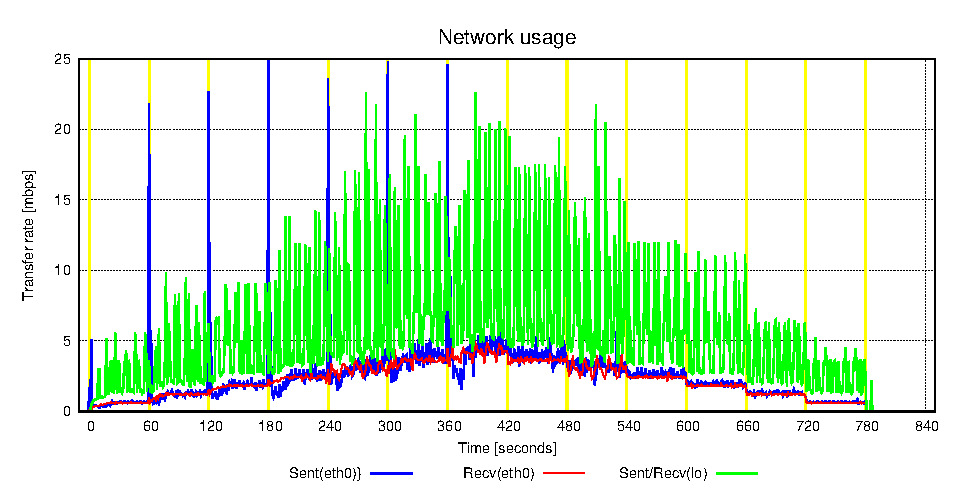
\includegraphics[width=\linewidth]{stats/test_full_features_net.eps}
  \caption{Network usage after implementing all features}
  \label{fig:test_full_features_net}
\end{figure}


      The blue peaks are caused by the signaling phase and web page downloads, including resources such as images, stylesheets and javascript files. 
      The green peaks are caused by video and audio being transfered between \gls{KMS} and \emph{MongoDB} through \emph{Kurento Repository}. Each peak occurs every time a block of video is recorded, which in this case is every ten seconds. 
      The recordings are synchronized so all user and mixed blocks start and end at the same time. That is why the amount of work done every ten seconds accumulates, and because this is performed locally, the maximum transfer rate is limited by the performance of the memory as buffers are written to buffers then to disks. 
      Sent data transfer rate has no significant peaks as \gls{HTTP} requests and signaling information contains little information.

	With this results we conclude that if we want to scale our storage solution using the \emph{MongoDB}'s cluster configuration, both \emph{Kurento Repository} and \gls{KMS} should be installed on the same machine because the loopback interface can handle bigger transfer rates than the remaining network interfaces. Installing the repository on the same machine as a database node does not ensure that recorded videos are stored in the same machine, for this reason we would prefer installing \gls{KMS} and \emph{Kurento Repository} on the same machine.





On the other hand, Figure \ref{fig:test_client_net} shows the respective network usage on the client side during our test case. We observe that in the first seconds the client adjusts the video quality it sends to \gls{KMS}. Whenever a new client enters the conference, we observe that \gls{KMS} decreases the video quality in order to instantaneously integrate a new user into the conference room. After a while, \gls{KMS} realizes that the network can handle the increase of clients and sends the video with a better quality to every participant. When a user leaves the conference room \gls{KMS} has no need to decrease the participant's video quality as less network bandwidth will be used.

\begin{figure}
  \centering
  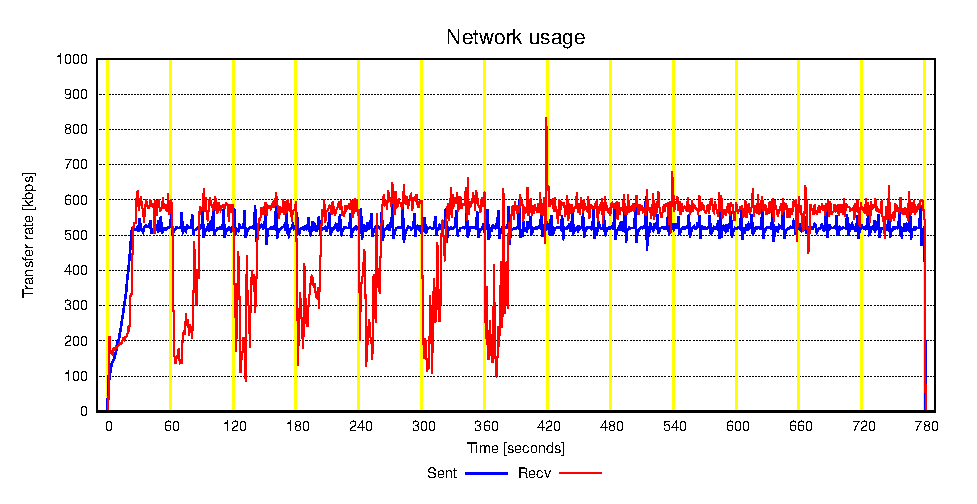
\includegraphics[width=\linewidth]{stats/test_client_net.eps}
  \caption{Client Network usage during our test case}
  \label{fig:test_client_net}
\end{figure}



\textbf{Memory usage}


Figure \ref{fig:test_ram_fixed_mem} shows the memory usage during our performance test. Both \gls{JVM}, \emph{MongoDB} and \gls{KMS} performs their own memory management by holding and recycling objects when needed. The expected and observed behavior of the memory usage is growth of memory usage while the users are entering the conference room and a memory usage stabilization afterwards.


\begin{figure}
  \centering
  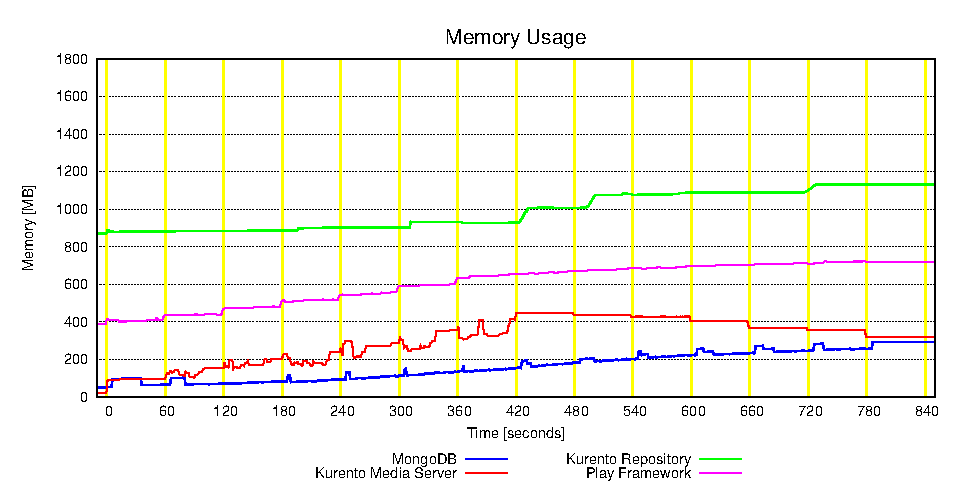
\includegraphics[width=\linewidth]{stats/test_ram_fixed_mem.eps}
  \caption{Memory usage after fixing recorder memory leak}
  \label{fig:test_ram_fixed_mem}
\end{figure}

\emph{MongoDB} memory usage keeps increasing because it tries to fit part of the database on \gls{RAM} for fast read access. \emph{MongoDB} checkpoints data to disk every 60 seconds or when journal data exceeds 2GB\footnote{\url{https://docs.mongodb.org/manual/faq/storage/}(Accessed March 28, 2016)}, that explains the small memory usage peaks during our test case. When the conference room is empty there are no video recordings, which explains the memory stabilization at the end.

\emph{KMS} memory management released resources as soon as users left the room. 


\textbf{CPU usage}


Figure \ref{fig:test_full_features_cpu} shows the percentage of \gls{CPU} usage during our performance test case. Each 100\% represents one \gls{CPU} core, although that does not mean one \gls{CPU} is fully used, for example two cores at 60\% represent 120\% \gls{CPU} usage. As we can see, the percentage of \gls{CPU} used increases and decreases linearly in function of the amount of conference participants. \gls{KMS} is responsible for most \gls{CPU} usage.


\begin{figure}
  \centering
  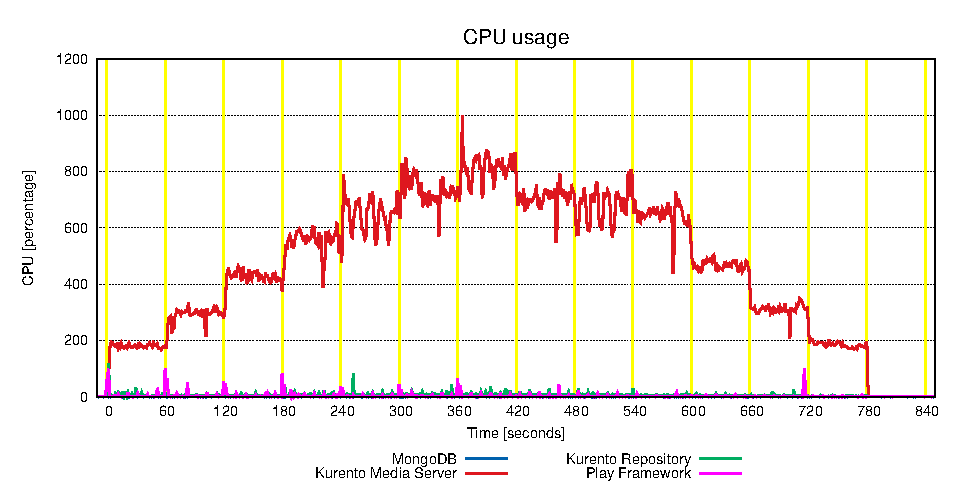
\includegraphics[width=\linewidth]{stats/test_full_features_cpu.eps}
  \caption{Percentage of CPU used during the performance tests}
  \label{fig:test_full_features_cpu}
\end{figure}

  Just for testing purposes, we performed the same performance tests disabling \gls{QR} codes detection. We concluded that \gls{QR} code detection is a very intensive task, approximately doubling the amount of work performed by the \gls{CPU}s.

	Even though, with this test results, we conclude that our solution's bottleneck is the \gls{CPU} usage at \gls{KMS}.



\subsection {Usability Tests}
     In this section we describe usability test scenarios that we have applied and their respective results.


    \subsubsection{Tests Scenarios}

      In order to evaluate the usability of our solution, we have performed usability tests with the help of real users with different backgrounds and ages.

      We handed a guide to the users with five tasks to perform. The metrics we used for each task were: number of clicks, number of errors (including a description) and time spent. 

  \subsubsection{Test Results}

In this section we present the results of our usability tests. The first time we tested our solution by providing tasks to users, we have observed that our solution was not perfect. Having faced usability problems during our tests, he had to improve our solution's usability and start the tests again.


In the first testing phase we have performed tests with just three users and ceased for improvements. We gathered comments and suggestions after letting the users explore our system.

On the second phase of our user interface tests, in a general way, we have noticed great improvements on the learning time.

In order to measure the users learning speed, we have performed tests with experienced users in order to retrieve the optimal task duration and minimal task clicks.

To this end, with regard to optimal task duration and minimal clicks, we obtained the values shown in Table \ref{table:optimal}.


\begin{table}[H]
\centering
\caption{Metrics for an experienced user}
\label{table:optimal}
\begin{tabular}{|c|c|c|c|c|c|}
\hline
\textbf{Task} & 1 & 2 & 3 & 4 & 5 \\ \hline
\textbf{Duration (seconds)} & 20 & 35 & 30 & 25 & 35 \\ \hline
\end{tabular}
\end{table}


From the data collected with twenty tests with users, namely the task duration (Figure \ref{fig:user_times}) and task difficulty (Figure \ref{fig:user_diffs}), we have calculated the confidence intervals in order to understand the most plausible values for each metric.

The youngest and oldest testers were, receptively, twenty two and thirty eight years old. Figure \ref{fig:user_ages} the ages of the users that tested our system.

\begin{figure}
  \centering
  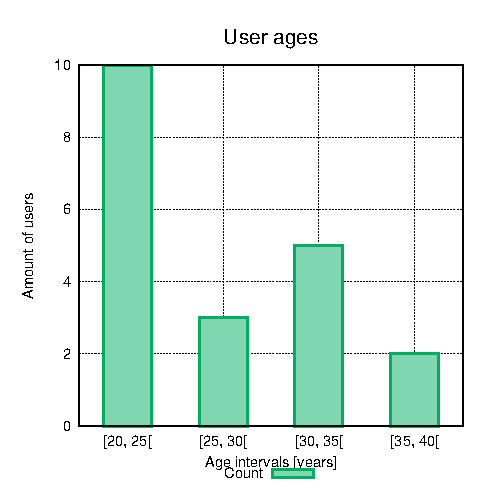
\includegraphics[width=0.8\linewidth]{stats/user_ages.eps}
  \caption{Ages of the users that tested our system}
  \label{fig:user_ages}
\end{figure}

As a result of both true average and variance being unknown and the usage of a relatively small amount of samples, we had to use \emph{t-distribution} to estimate our metrics confidence intervals. We have used a 95\% confidence level.

\begin{figure}
  \centering
    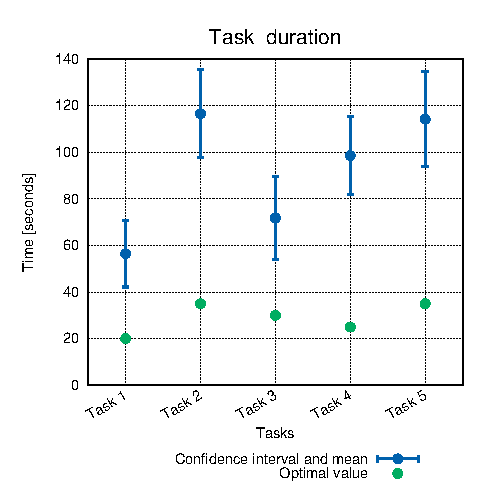
\includegraphics[width=0.8\linewidth]{stats/user_times.eps}
    \caption{Time spent per task}
    \label{fig:user_times}
\end{figure}

According to Figure \ref{fig:user_diffs}, we can observe that most users had less difficulties with the first two tasks, which represents types of tasks that most users are familiar with. As soon as users had to navigate in time, manipulate annotations and create content (respectively \emph{task3}, \emph{task4} and \emph{task5}) we observed that they revealed more difficulties. Most of those difficulties, based on the users feedback, were mainly due to those concepts not being familiar to them.



\begin{figure}
  \centering
    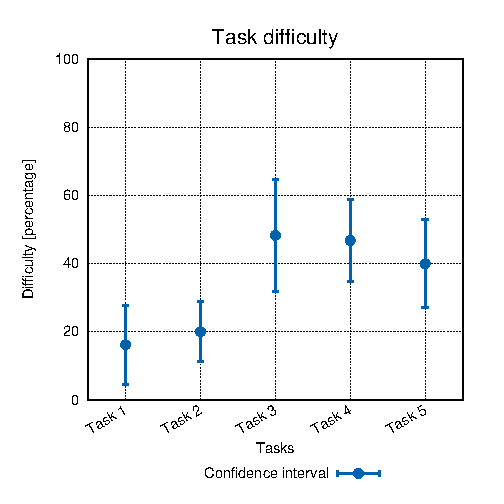
\includegraphics[width=0.8\linewidth]{stats/user_diffs.eps}
  \caption{Difficulty per task}
  \label{fig:user_diffs}
\end{figure}


As we had relatively bad results with some users, we explained to those users that could not conclude the tasks or performed them incorrectly, the most efficient way to perform the requested tasks. Some users suggested to display more hints in order to achieve a faster learning, but afterwards all were impressed and gave us a better evaluation.

Most users gave us worse evaluations on our user interface layout and content editor, which was due to having a lot of tools present in the same web page and some of them being hidden due the screen size. In some cases users had to scroll down in order to find the tools they were looking for. 

Another weak aspect was our content editor, which, in fact, we recognize is difficult to work with, mostly due to the amount of information that is necessary to create a synchronized content (starting time, duration and content itself). Some users have suggested that the content should also be present on the timeline so they could be easily dragged and resized (on time).

We are aware that placing content on the timeline will reduce our solutions performance, especially when there is a relatively large amount of content, due to the content that is present on the timeline being loaded all at once. Although, we recognize that for some cases (relatively low amount of content), displaying the content on the timeline could not have a great impact on our solutions performance, we choose not to implement this.

In conclusion, 100\% of our testers though that our solution was an innovation and 95\% recommended using our solution.




\section{Conclusions}
\label{chapter:conclusion}
\subsection{Achievements}
\label{section:achievements}

	We have successfully implemented the basic functionalities of our prototype and spare some time for adding more valuable features such as the ability to create content by exposing \gls{QR} codes to the camera and lastly perform changes to the user interface in order to improve the quality of user's experience.

	The performance tests that we have executed showed that our system is stable and more importantly that our web server is lightweight and most of processing power is dedicated to the streaming server.

	Our usability tests show results that are considerably worse than the established optimal values due to our solution propose a different way to communicate that most people are not used to. Although we have obtained those results, in general our users gave us positive feedback and valuable advices which we have used to improve our system. 

\subsection{Future Work}
\label{section:future}
	Playing back video with a faster rate is not possible using the current version of \gls{KMS}. Even though we expect the availability of that feature in a near future but we have proposed an alternative way to implement faster playback by using \emph{ffmpeg} to convert the video before playing it.

	Although we have tested our solution in a powerful machine for the current time, our performance tests revealed that the streaming component uses a lot of resources. We left for a future work a deep analysis on the scalability of our system for which we have proposed different approaches but we have not tested them.

	Another aspect we could have tested was the performance of our solution when using \gls{TURN} servers for relaying the traffic that fails using \gls{STUN}.

	Lastly, we have chosen functionality over security in respect to displaying content to users which lead to security flaws on our solution. Although we have not solved the security problems, we have proposed a solution which at the same time limits the flexibility of adding new functionalities to our prototype.




%Sets the bibliography style to UNSRT and imports the 
%bibliography file "samples.bib".
%\bibliographystyle{unsrt}
%\bibliography{references}

%%%%%%%%%%%%%%%%%%%%%%%%%%%%%%%%%%%%%%%%%%%%%%%%%%%%%%%%%%%%%%%%%%%%%%%%%
%     This file should not be altered                                  %
%     To see what other .tex files search for TODO word                %
%     If more chapters are required, add more \inputs{file} commands   %
%%%%%%%%%%%%%%%%%%%%%%%%%%%%%%%%%%%%%%%%%%%%%%%%%%%%%%%%%%%%%%%%%%%%%%%%
\documentclass[10pt,a4paper,twoside]{report}

% TODO - change this with your external packages (if required)
% ----------------------------------------------------------------------
% Define document language.
% ----------------------------------------------------------------------
% Select one
%\usepackage[latin1]{inputenc} % <<<<< Windows
\usepackage[utf8]{inputenc}   % <<<<< Linux

% Select one
%\usepackage[portuguese]{babel} % <<<<< Portuguese
\usepackage[english]{babel} % <<<<< English

% List of LaTeX variable names: \abstractname, \appendixname, \bibname,
%   \chaptername, \contentsname, \listfigurename, \listtablename, ...)
% http://www.tex.ac.uk/cgi-bin/texfaq2html?label=fixnam
%
% Changing the words babel uses (uncomment and redefine as necessary...)
\newcommand{\acknowledgments}{@undefined} % new LaTeX variable name
%
% > English
%
\addto\captionsenglish{\renewcommand{\acknowledgments}{Acknowledgments}}
%\addto\captionsenglish{\renewcommand{\listtablename}{List of Tables}}
%\addto\captionsenglish{\renewcommand{\listfigurename}{List of Figures}}
%\addto\captionsenglish{\renewcommand{\nomname}{Nomenclature}}
%\addto\captionsenglish{\renewcommand{\appendixname}{Appendix}}
%\addto\captionsenglish{\renewcommand{\bibname}{References}} % Bibliography

% > Portuguese
%
\addto\captionsportuguese{\renewcommand{\acknowledgments}{Agradecimentos}}
%\addto\captionsportuguese{\renewcommand{\listtablename}{Lista de Figuras}}
%\addto\captionsportuguese{\renewcommand{\listfigurename}{Lista de Tabelas}}
\addto\captionsportuguese{\renewcommand{\nomname}{Lista de S\'{i}mbolos}} % Nomenclatura
%\addto\captionsportuguese{\renewcommand{\appendixname}{Anexo}} % Apendice
%\addto\captionsportuguese{\renewcommand{\bibname}{Refer\^{e}ncias}} % Bibliografia


% ----------------------------------------------------------------------
% Define default and cover page fonts.
% ----------------------------------------------------------------------

% Use Arial font as default
%
\renewcommand{\rmdefault}{phv}
\renewcommand{\sfdefault}{phv}

% Define cover page fonts
%         encoding     family       series      shape
%  \usefont{T1}     {phv}=helvetica  {b}=bold    {n}=normal
%                   {ptm}=times      {m}=normal  {sl}=slanted
%                                                {it}=italic
% see more examples at
% http://julien.coron.free.fr/languages/latex/fonts/
%
\def\FontLn{% 16 pt normal
  \usefont{T1}{phv}{m}{n}\fontsize{16pt}{16pt}\selectfont}
\def\FontLb{% 16 pt bold
  \usefont{T1}{phv}{b}{n}\fontsize{16pt}{16pt}\selectfont}
\def\FontMn{% 14 pt normal
  \usefont{T1}{phv}{m}{n}\fontsize{14pt}{14pt}\selectfont}
\def\FontMb{% 14 pt bold
  \usefont{T1}{phv}{b}{n}\fontsize{14pt}{14pt}\selectfont}
\def\FontSn{% 12 pt normal
  \usefont{T1}{phv}{m}{n}\fontsize{12pt}{12pt}\selectfont}

% Define page margins and line spacing.
% set the page margins (2.5cm minimum in every side, as per IST rules)
\usepackage{geometry}
\geometry{verbose,tmargin=2.5cm,bmargin=2.5cm,lmargin=2.5cm,rmargin=2.5cm}

% Set space between lines.
% allow setting line spacing (line spacing of 1.5, as per IST rules)
\usepackage{setspace}
\renewcommand{\baselinestretch}{1.5}


% ----------------------------------------------------------------------
% Include external packages.
\usepackage{graphicx}

% Include acronyms
\usepackage{acronym}

% Mathematical enhancements for LaTeX.
\usepackage{amsmath}  % AMS mathematical facilities for LaTeX.
\usepackage{amsthm}   % Typesetting theorems (AMS style).
\usepackage{amsfonts} %
%\usepackage{cancel}
\usepackage[normalem]{ulem}

% 'subfigure' package
%
% Deprecated: Figures divided into subfigures.
% http://www.ctan.org/tex-archive/obsolete/macros/latex/contrib/subfigure/
%
% > subcaptions for subfigures
%
\usepackage{subfigure}
\usepackage{flafter}

% 'subfigmat' package
%
% Automates layout when using the subfigure package.
% http://www.ctan.org/tex-archive/macros/latex/contrib/subfigmat/
%
% > matrices of similar subfigures
%
\usepackage{subfigmat}


% 'url' package
%
% Verbatim with URL-sensitive line breaks.
% http://www.ctan.org/tex-archive/macros/latex/contrib/url/
%
% > URLs in BibTex
%
% \usepackage{url}


% 'rotating' package
%
% Rotation tools, including rotated full-page floats.
% http://www.ctan.org/tex-archive/macros/latex/contrib/rotating/
%
% > show wide figures and tables in landscape format:
%   use \begin{sidewaystable} and \begin{sidewaysfigure}
%   instead of 'table' and 'figure', respectively.
%
\usepackage{rotating}


% 'hyperref' package
%
% Extensive support for hypertext in LaTeX.
% http://www.ctan.org/tex-archive/macros/latex/contrib/hyperref/
%
% > Extends the functionality of all the LATEX cross-referencing
%   commands (including the table of contents, bibliographies etc) to
%   produce \special commands which a driver can turn into hypertext
%   links; Also provides new commands to allow the user to write adhoc
%   hypertext links, including those to external documents and URLs.
%
\usepackage[pdftex]{hyperref}              % enhance documents that are to be output as HTML and PDF
\hypersetup{colorlinks,                    % color text of links and anchors, eliminates borders around links
            % linkcolor=red,               % color for normal internal links
            linkcolor=black,               % color for normal internal links
            anchorcolor=black,             % color for anchor text
            % citecolor=green,             % color for bibliographical citations
            citecolor=black,               % color for bibliographical citations
            % filecolor=magenta,           % color for URLs which open local files
            filecolor=black,               % color for URLs which open local files
            % menucolor=red,               % color for Acrobat menu items
            menucolor=black,               % color for Acrobat menu items
            % urlcolor=cyan,               % color for linked URLs
            urlcolor=black,                % color for linked URLs
            % bookmarks=true,              % create PDF bookmarks (by default is true)
	        bookmarksopen=false,           % do not expand bookmarks
	        bookmarksnumbered=true,        % number bookmarks
	        pdftitle={Thesis},             % TODO Change to your thesis title
            pdfauthor={TODO},              % TODO Change to your name
            pdfsubject={TODO },            % TODO Change to your thesis subject
            pdfkeywords={TODO },           % TODO Change to thesis keywords
            pdfstartview=FitV,
            pdfdisplaydoctitle=true}


% 'hypcap' package
%
% Adjusting the anchors of captions.
% http://www.ctan.org/tex-archive/macros/latex/contrib/oberdiek/
%
% > fixes the problem with hyperref, that links to floats points
%   below the caption and not at the beginning of the float.
%
\usepackage[figure,table]{hypcap}

% ----------------------------------------------------------------------
% Define new commands to assure consistent treatment throughout document
% ----------------------------------------------------------------------
\newcommand{\degree}{\ensuremath{^\circ\,}} % degrees


% If you need a numbered subsubsubsection uncomment the following lines
% \setcounter{secnumdepth}{4}
% \setcounter{tocdepth}{2}                 % Refrains ToC to two levels
% \def\subsubsubsection#1{\paragraph{#1}~\\}



\usepackage{amssymb}
\usepackage{makeidx}  % allows for indexgeneration
\usepackage{kmath}  % allows for indexgeneration
\usepackage{color}  % allows for indexgeneration
\usepackage[dvipsnames]{xcolor}
\usepackage{url}
\usepackage{array}
\usepackage{hyperref}
\usepackage{graphicx}
\usepackage{caption}

\usepackage{float}
\usepackage{mathtools}
\usepackage{acronym}
\usepackage{pgfgantt}
\usepackage{adjustbox}
\usepackage{rotating}
\usepackage{listings}
\usepackage{dirtytalk}
\usepackage[graphicx]{realboxes}
\definecolor{fade}{rgb}{0.8,0.8,0.8}
\usepackage{tabularx} % in the preamble
\usepackage{xcolor}

\usepackage{tikz}
\usepackage{pgf-umlsd}
\usepackage{textcomp}
\usepackage{environ}
\usepackage{graphics}
\usepackage{pgfplots} 
\pgfplotsset{compat=1.9}

\newcolumntype{M}[1]{>{\centering\arraybackslash}m{\linewidth/#1}}
\newcolumntype{Y}{>{\centering\arraybackslash}X}


%\overfullrule=2cm

\usetikzlibrary{positioning,shapes,shadows,arrows,matrix,decorations.pathreplacing,external}
\tikzexternalize
\tikzset{external/mode=graphics if exists}

\newganttchartelement*{mymilestone}{
mymilestone/.style={
shape=isosceles triangle,
inner sep=0pt,
draw=cyan,
top color=white,
bottom color=cyan!50
},
mymilestone incomplete/.style={
/pgfgantt/mymilestone,
draw=yellow,
bottom color=yellow!50
},
mymilestone label font=\slshape,
mymilestone left shift=0pt,
mymilestone right shift=0pt
}

\newgantttimeslotformat{stardate}{%
\def\decomposestardate##1.##2\relax{%
\def\stardateyear{##1}\def\stardateday{##2}%
}%
\decomposestardate#1\relax%
\pgfcalendardatetojulian{\stardateyear-01-01}{#2}%
\advance#2 by-1\relax%
\advance#2 by\stardateday\relax%
}




\lstdefinelanguage{JavaScript}{
  keywords={break, case, catch, continue, debugger, default, delete, do, else, false, finally, for, function, if, in, instanceof, new, null, return, switch, this, throw, true, try, typeof, var, void, while, with},
    numbers=left,
    numberstyle=\scriptsize,
  morecomment=[l]{//},
  morecomment=[s]{/*}{*/},
  morestring=[b]',
  morestring=[b]",
      stepnumber=1,
    numbersep=8pt,
    showstringspaces=false,
    breaklines=true,
    frame=lines,
    backgroundcolor=\color{background},
  ndkeywords={class, export, boolean, throw, implements, import, this},
  keywordstyle=\color{blue}\bfseries,
  ndkeywordstyle=\color{darkgray}\bfseries,
  identifierstyle=\color{black},
  commentstyle=\color{purple}\ttfamily,
  stringstyle=\color{red}\ttfamily,
  sensitive=true
}

\usepackage{color, colortbl}
\definecolor{Gray}{gray}{0.9}

\colorlet{punct}{red!60!black}
\definecolor{background}{HTML}{FFFFFF}
\definecolor{delim}{RGB}{20,105,176}
\colorlet{numb}{magenta!60!black}
\definecolor{grisbg}{gray}{0.95}

\lstdefinelanguage{json}{
    %basicstyle=\normalfont\ttfamily,
  keywords={data, cmd},
    numbers=left,
    numberstyle=\scriptsize,
    morestring=[b]',
    morestring=[b]",
    stepnumber=1,
    numbersep=8pt,
    showstringspaces=false,
    breaklines=true,
    frame=lines,
    backgroundcolor=\color{background},
    literate=
     *{0}{{{\color{numb}0}}}{1}
      {1}{{{\color{numb}1}}}{1}
      {2}{{{\color{numb}2}}}{1}
      {3}{{{\color{numb}3}}}{1}
      {4}{{{\color{numb}4}}}{1}
      {5}{{{\color{numb}5}}}{1}
      {6}{{{\color{numb}6}}}{1}
      {7}{{{\color{numb}7}}}{1}
      {8}{{{\color{numb}8}}}{1}
      {9}{{{\color{numb}9}}}{1}
      {:}{{{\color{punct}{:}}}}{1}
      {,}{{{\color{punct}{,}}}}{1}
      {\{}{{{\color{delim}{\{}}}}{1}
      {\}}{{{\color{delim}{\}}}}}{1}
      {[}{{{\color{delim}{[}}}}{1}
      {]}{{{\color{delim}{]}}}}{1},
 keywordstyle=\color{blue}\bfseries,
  ndkeywordstyle=\color{darkgray}\bfseries,
  identifierstyle=\color{black},
  commentstyle=\color{purple}\ttfamily,
  stringstyle=\color{red}\ttfamily,
  sensitive=true
}




\begin{document}

% Set plain page style (no headers, footer with centered page number)
\pagestyle{plain}

% Set roman numbering (i,ii,...) before the start of chapters
\pagenumbering{roman}

% TODO Define your cover page
\thispagestyle {empty}

% IST Logo
% parameters: bb=llx lly urx ury (bounding box), width=h_length, height=v_length, angle=angle, scale=factor, clip=true/false, draft=true/false. 
\newgeometry{left=2cm,top=2.5cm, right=2.5cm, bottom=0cm}

\includegraphics[width=5.0cm]{Logo.png}

\begin{center}
%
% Figure (Image or plot)
\vspace{0.3cm}
% TODO - Use of an image is optional
\hspace{-0.5cm}
\includegraphics[height=50mm]{Figures/logo.png}
% TODO - If you don't use an image uncomment the next line
% \vspace{5.0cm}

% Title, author and degree
\vspace{0.8cm}
{\FontLb Hyper-linked Communications: WebRTC enabled asynchronous collaboration} \\
%\vspace{0.2cm}
%{\FontMn Subtítulo (facultativo)} \\
%\vspace{1.9cm}
\vspace{2.6cm}
{\FontMb Henrique Duarte Lopes Rocha} \\
\vspace{1.9cm}
{\FontLn Disserta\c{c}\~{a}o para a obten\c{c}\~{a}o de Grau de Mestre em} \\
\vspace{0.3cm}
{\FontLb Engenharia de Telecomunicações e Informática} \\
\vspace{1.9cm}
{\FontMb J\'{u}ri} \\
\vspace{0.3cm}
{\FontSn %
Presidente:        Nome do Presidente \\
Orientador:        Nome do Orientador \\
Co-orientador:     Nome do Co-orientador \\
Vogais:            Nome do Vogal 1 \\
                   Nome do Vogal 2 \\
}
\vspace{1.5cm}

{\FontMb M\^{e}s e Ano} \\
%
\end{center}

\cleardoublepage

\restoregeometry


% TODO Dedication page (optional, and not normal)
% \input{Thesis_Dedication} % Uncomment if it is used

% TODO Acknowledgments (optional and can be in native language)
\chapter*{\acknowledgments}

% Add entry in the table of contents as chapter
\addcontentsline{toc}{chapter}{\acknowledgments}

I would like to thank my dissertation supervisor Ricardo Pereira and co-supervisor Paulo Chainho for their active support and ideas that were crucial for the development of this thesis.

I should not forget all the people involved on the prototype's test phase, they not only tested but also gave valuable feedback that we used to improve the quality of our prototype. 

Also, I would like to show my gratitude to the \emph{Kurento} team for developing the streaming server that I've used, their impressive help support and receptiveness to discuss new functionalities.   

Not less important I should thank all IST employees that maintained the space I used during this journey.

Lastly, I should thank all the people that supported me psychologically and made me going my own way. 

Thank you!

\cleardoublepage

% TODO Abstract in English and Portuguese
\chapter*{Abstract}

% DO NOT CHANGE THIS - Add entry in the table of contents as chapter
\addcontentsline{toc}{chapter}{Abstract}

The Hyper-linked communications concept applies much of the hypermedia concepts, widely used on Web content, to communication and collaboration services. This paradigm allows to synchronize, structure and navigate communication content, providing a way to integrate social media content and collaborative tools into voice and video calls.
Voice and image together can express emotions and expose creativity like no other medium can. With hypermedia concepts, we can add more value to voice and video communications.

\emph{WebRTC} technology allows real-time communications between web browsers without the need to install and use additional applications or plug-ins. The nature of web browser applications already follows the hypermedia concept, which makes \emph{WebRTC} the ideal technology to apply the hyper-linked communications concepts.
{\color{blue}The web browser platform provides an abstraction layer that makes it possible to create applications that run independently from the operating system.}
The native support for \emph{WebRTC} in operating systems extends its usage to outside the web browser, allowing for the exploration of functionalities for which web browsers provide poor support, such as video recording and massive information storage.

%\sout{Our goal in this project is to develop an application that leverages the Hyper-linked communications concept to enable collaborative real-time audio and video communication, enriched with other media types, that can be accessed live or accessed later.}
%This application will target the web browser platform, resorting to \ac{WebRTC}.


{\color{red}Our goal in this project is to develop an application targeted to the web platform, resorting to \emph{WebRTC}, that leverages the hyper-linked communications by providing a video conference environment enriched with interactive and non-interactive discrete media types.}

{\color{red}One of the key features of this project is the ability to navigate in time in order to reproduce the conversation again or introduce hyper-content to it such as time annotations, interactive lists of topics and subtitles. In this context we also provide a simpler method for creating and synchronizing hyper-content using \emph{QR codes}.}

{\color{red}In addition to this conference environment, which provides different functionalities than traditional conference environments such as \emph{Skype} and \emph{Google Hangouts}, we also enable a collaborative text editor and a chat that supports sending time hyper-links and files to conference participants.}

{\color{red}Furthermore, another relevant feature is the possibility to compose multiple video streams into a single one, which enables adding more users to conference rooms without impacting on clients performance. Users can change to individual streams on demand or automatically to the talking users.}


%RP acho que estás a vender muito mal o teu trabalho. O abstract é a primeira caisa que se lê e em função disso decidimos se lemos mais ou não. Tens aqui a oportunidade de chamar a atenção para algumas das funções inovadoras. O texto está muit genérico. podes falar em coisas concretas: video conferência, chat, edição colaborativo de documento, partilha de ficheiros, possibilidade de criar legendas, tags, etc. Possibilidade de navegar, voltar atrás, etc como no IPTV. Gestão de amigos, gerir salas, etc, etc.

{\color{blue}
In this document, we present the current State Of The Art in hyper-linked communications and related technologies, propose and implement an architecture for an hyper-linked communication application based on \emph{WebRTC} and provide the results for its implementation and evaluation.
}

%RP em vez de ``provide the results for its implementation and evaluation'', diz algo como: ``this work was evaluated using a panel of 20 users, who reported that they liked to use it and thought it to be extremelly inovative ... and if given the change, would use it ...''

\vspace{1cm}

% TODO 4 to 6 keywords;
\textbf{\Large Keywords:} WebRTC, asynchronous, communications, collaboration


\cleardoublepage


% ----------------------------------------------------------------------
%  Table of contents, list of tables, list of figures and nomenclature
%  (DO NOT TOUCH THIS!!!)
% ----------------------------------------------------------------------

% Table of contents
\tableofcontents
\cleardoublepage

% List of figures
\listoffigures
\addcontentsline{toc}{chapter}{\listfigurename}
\cleardoublepage

% List of tables
\listoftables
\addcontentsline{toc}{chapter}{\listtablename}
\cleardoublepage

\section*{}
\addcontentsline{toc}{chapter}{Acronyms}
\section*{List of Acronyms}
\begin{acronym}
\acro{IEEE}{Institute of Electrical and Electronics Engineers}
\acro{SMTP}{Simple Mail Transfer Protocol}
\end{acronym}

\cleardoublepage

% Set arabic numbering (1,2,...) after preface
\setcounter{page}{1}
\pagenumbering{arabic}

% ----------------------------------------------------------------------
%  TODO - Edit each chapters file and create new if necessary
% ----------------------------------------------------------------------

\chapter{Introduction}
\label{chapter:introduction}
%The introduction is certainly the most read section of any deliverable, and it largely determines the attitude of the reader/reviewer will have toward the work. Therefore, it is probably the most delicate part of the writing of a report.

\section{Background}
\label{section:background}
%Nesta secção devem descrever a área em que a vossa tese se insere, de forma a contextualizar o problema que vão resolver. No âmbito da área devem identificar os principais problemas que existem.

	Since the early days of Human History, we tried to communicate over far locations, from smoke signals to letters delivered by messengers. Real-time communications were limited or even nonexistent. Despite all the efforts made to improve communications, written communication could never replace face to face communication.
	With the advent of the telephone network, communications have taken a very important step for us to feel more connected with whom we communicate. Still, only the human voice was not enough, and the invention of cameras and consequent video digitalization were a huge step for real-time communications.

	In the past, handwritten documents were limited to a writer per page at a time. Writing a book collaboratively was a difficult task due to synchronization between writers.
	Today, we can achieve more. It is possible to write a document collaboratively, correct spelling mistakes without wasting physical resources, restructure text at any moment, add a video to a newspaper article and more. Although much of what was said seems banal nowadays, none of this was possible before the computer's invention. 

	As Martin Geddes states\cite{geddes}, \say{No computer in our lifetimes will ever rival a human voice's capacity to conveying rich and complex social and emotional meaning}. Although nothing replaces the physical contact with a person while we communicate, we are at a time when we can do more than just visual and verbal communication. Hypermedia can be added to video and voice in order to extend its value. The concept of structured voice and video synchronized with hypermedia is called hypervoice\cite{geddes}.

     

\section{Proposed Solution}
\label{section:proposed}

	As communications technologies appeared, we adapted the way we communicate. {\color{blue} The purpose of this project is not the replacement of} the current video and audio communications, but to enrich them with hyper-media content and make them a more natural and easy to learn process. 

	{\color{blue}With the advent of WebRTC and its successive integration with web browsers, it became possible to develop video conference web applications without plugins, this presents a range of possibilities on what can be implemented using already existing web technologies.}
		
    Furthermore, real-time communication applications can make a significant difference on business, education and health sectors by providing tools for developing teaching and learning online, teamworking and socializing web applications.

	For multiple reasons, we often need to repeat or postpone some of our tasks, some people tend to forget what they ear or see.
        %RP Parece-me que até aqui ainda é background ou motivação. Não me parece que estejas já a descrever a solução proposta.
        
	Therefore, a real-time system is a huge source of information that requires much attention from its users. In this context, an application that provides a way to remember our past communications would be a strong tool for not only to catch what we lost but also to enhance our knowledge.


	{\color{blue}Another point to consider is making available collaborative tools for text edition, instant messaging and video superimposed content creation and visualization.}


        

\section{Thesis Contribution}
\label{section:contribution}
%Nesta secção devem identificar como é que a vossa solução vai contribuir para resolver o problema.

Making it clear, this project aims to complement current audio, text and video communications in order to create rich and collaborative interfaces with the ability to add more content on a future time (e.g. creating time annotations for improving content search) in order to increase its value. It is also important to highlight another goal of this project which is the ability to navigate in time by rewinding communications, fast-forward and jump to certain points.

%RP Estás a misturar goals com contribuições. Nesta altura deves falar do que foi feito (na solução). Os objectivos podem ficar no inicio da arquitectura para a motivar e condicionar 

A web application with an easy to learn user interface will be developed to accomplish solving our problem. Our application, unnamed yet, is targeted at web browsers that are compatible with only standard technologies like JavaScript, \ac{WebRTC}, \ac{HTML}5 and \ac{CSS}3. Any additional plug-in is avoidable, \emph{JavaScript} libraries will be preferred as they can be downloaded on the fly.

%RP ``will be developed''!!! ``was''. Não podes estar a falar no futuro. Isto é passado. Estás a descrever o que fizeste.

	Although we propose an initial solution to solve our problem, we will make a continuous effort to survey the systems that solve our problem either completely or just a part of it, not excluding solutions that may appear during the implementation of our project.

	We will present an architecture that can meet our goals, implement the respective prototype and test it with real users and performance benchmarks.

        %RP mais uma vez, passado e muito vago.
        
	According to Martin Geddes, the quality of the interaction worsens as the number of users increase\cite{geddes}. In our testing phases we will quantify and qualify the impact of increasing users on the interface and performance of our prototype. 

	All the problems faced during the development and limitations will be reported on the thesis so that a future project better then ours can be easily and better developed.

        %RP este capítulo precisa de uma revisão. A estrutura tem de ser:
        %Motivação/background - descrever os problemas / desafios / oportunidades que motivam a tese
        %Proposed solution - descrever por alto a solução para o problema, uma aplicação web com determinadas funcionalides (listando todas elas)
        %contribution - as contribuições são: uma arquitectura, um interface utilizador para lidar com um conceito novo (andar no tempo), um protótipo funcional, teste com utilizadores e respectivas conclusões (avaliação experimental), documentação (tese).

\section{Outline}

This rest of this document is structured as follows:

\begin{itemize}
%\item \textbf{Chapter \ref{chapter:introduction}} presents the motivation, background and proposed solution.
\item \textbf{Chapter \ref{chapter:relatedwork}} describes the previous work in the field.
\item \textbf{Chapter \ref{chapter:architecture}} describes the system requirements and the architecture for an Web Application that fulfills the goals of this thesis.
\item \textbf{Chapter \ref{chapter:implementation}} describes the implementation of our Web Application and the technologies chosen.
\item \textbf{Chapter \ref{chapter:evaluation}} presents the evaluation tests performed and the corresponding results.
\item \textbf{Chapter \ref{chapter:conclusion}} summarizes the work developed and proposes future work.
\end{itemize}

\cleardoublepage
 % file "Thesis_Introduction.tex"

\chapter{Related Work}
\label{chapter:relatedwork}

\section{Related Work}\label{related}
 This section is structured as follows.
 Section \ref{early} describes the problems that real-time communications face on nowadays internet, namely the \ac{IPv4} address exhaustion and the client server model constraints. 
 Section \ref{rtc} describes the \ac{WebRTC} technology and the protocols needed to implement our project. 
 Section \ref{signaling} addresses the signaling component of chat applications, which is not defined on \ac{WebRTC} specifications. 
 Section \ref{hypermedia} presents the evolution of multimedia content until the hypermedia, its capabilities, synchronization mechanisms and interactivity. 
 Section \ref{collab} explores streaming protocols for non-interactive multimedia and how to introduce the interactive component, another important aspects are the ability to control the time flux of a stream and collaborative application development.
%RP este detalhe sobre a estrutura da sec. do estado da arte vai para o início dessa secção.
        

\section{Early days of the Internet and its remaining flaws}\label{early}

The need to build a global communications network in an age when almost nobody had access to that technology and the unpredictability of the number of future users, lead to some protocols not being suitable for the explosive growth and proliferation of users that followed. \ac{IPv4} limits the number of public addresses in such a way that today they are scarce \cite{ipv4}. Today we live in the \ac{IoT} era.
  Users and companies may have multiple devices that require Internet connectivity, such as personal computers, smartphones, tablets, traffic sensors, public surveilance systems, health monitoring tools and so on. All those devices combined cannot be publicly addressed by \ac{IPv4}.
%RP vigillance -> surveilance?
%RP usa acrónimo IoT para Internet of Things

To this end, one way to overcome the \ac{IPv4} address scarcity problem was the development of a mechanism that groups multiple address into a single one, the machine that is assigned that address is then responsible for redirecting messages to members of its group using their private addresses, each connection in the private network is identified publicly by the same \ac{IP} address with a different port.
%RP o porto não identifica uma máquina (membro da rede privada) mas uma ligação.
This technique is known as \ac{NAT} (figure \ref{fig:nat}).

\begin{figure}
	\centering
	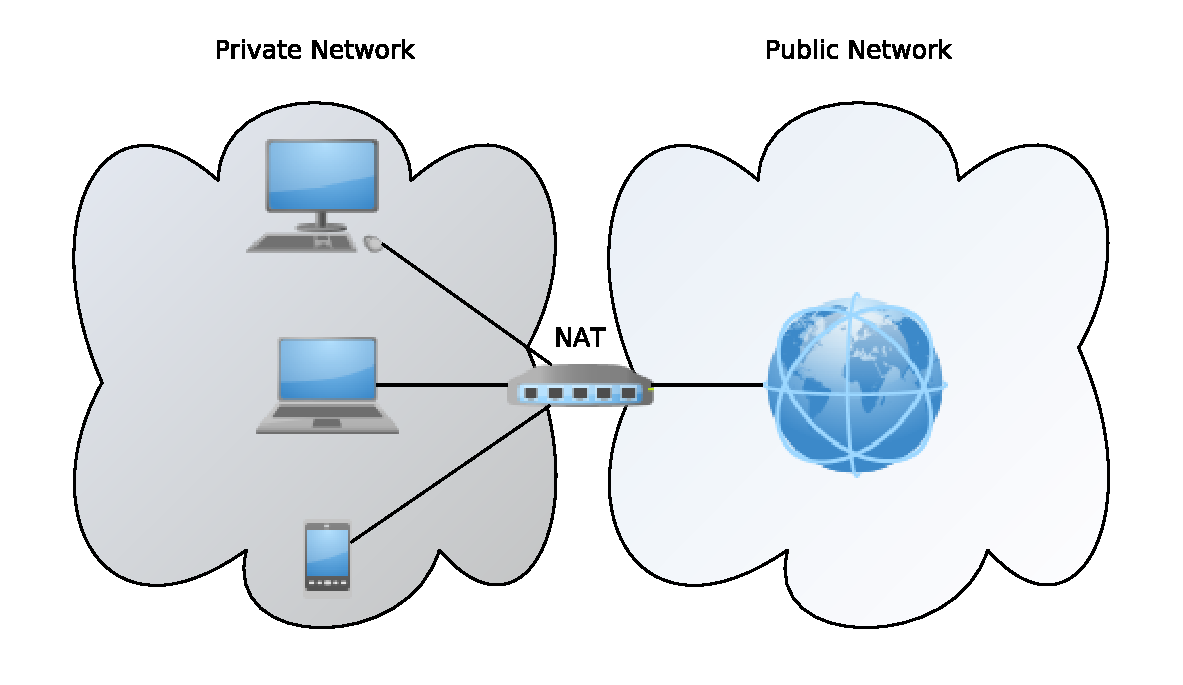
\includegraphics[width=0.7\textwidth]{figures/nat.pdf}
	\caption{Network Address Translation}
	\label{fig:nat}
\end{figure}
%RP na figura devias indicar que uns tem ips publicos e outros privados. Alternativamente, colocavas metade da nat box dentro da núvem para indicar que esta pertence à Internet e os pc não. 

Initially \ac{NAT} offered an alternative to address exhaustion and a minimal sensation of security.
However, due to their current wide usage, \ac{NAT}s weaknesses are being exposing at the application layer, namely impacting applications that require direct communications between two private networks.

There are four types of \ac{NAT} implementations\cite{rfc3489}: \emph{Full Cone NAT}, \emph{Restricted Cone NAT}, \emph{Port Restricted Cone NAT}, \emph{Symmetric NAT}.

\emph{Full Cone} \ac{NAT} maps each public \ac{IP} address and port to a private \ac{IP} address and port.
Any external host can communicate with private hosts through their mapped public address and port. This represents the least restrictive type of \ac{NAT} and, as we will see later, the unique type of \ac{NAT} that enables real time communications from point to point.

\emph{Restricted Cone} \ac{NAT} requires that a private client must first send a message to an external host before it can receive messages from the same host. With this type of \ac{NAT}, the private client can be contacted from any port of the same external host.

\emph{Port Restricted Cone} \ac{NAT} works in the same way as Restricted Cone \ac{NAT}, but it only allows communications from the same external host's IP address and port, ignoring all messages from other applications within the same external host.

\emph{Symmetric} NAT maps different ports for each connection. As we will see later, this type of \ac{NAT} represents a problem on real time communications.

\emph{Non-Symmetric} \ac{NAT}s became the common configurations on the Internet. As a direct result, problems started to appear: the amount of ports that \ac{IP} makes available is also small compared to our current needs; worse than that, \ac{NAT} also difficults end-to-end communication, forcing most applications that follow this model to be implemented ineffectively.

Unless the router that performs as \ac{NAT} has forwarding rules to every desired ports of each user, applications behind a \ac{NAT} are prevented from receiving incoming connections from the public network, which forces them to behave as a client of a client-server model. 

Applications based on multimedia and peer-to-peer file sharing have been one of the most strained by the \ac{NAT} technique. It is also important to highlight that those kind of applications require real time communication in order to achieve the best performance.

\begin{figure}
	\centering
	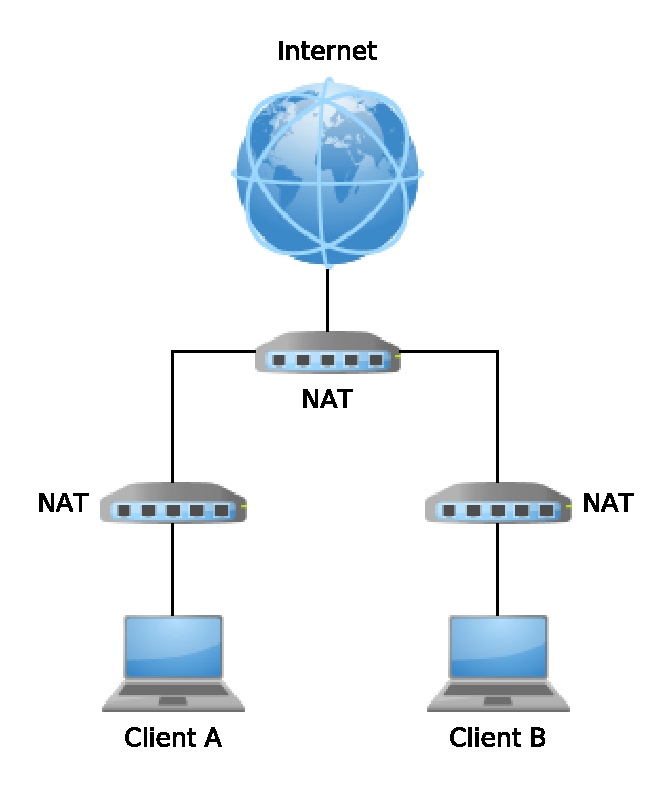
\includegraphics[width=0.45\textwidth]{figures/multinat.pdf}
	\caption{Multiple level NATs}
	\label{fig:multinat}
\end{figure}

\ac{STUN} and \ac{TURN} \cite{natvoip} servers are a possible solution to overcome \ac{NAT}. None of those can establish direct connections on multiple level \ac{NAT}s (figure \ref{fig:multinat}).
%RP explicar o que são multiple level pois não falaste disto antes? São ``nested''?

\ac{STUN} servers are quite simple. They receive requests from \ac{NAT}ed clients, with the source address of a request being the public address that \ac{NAT} mapped to the client. \ac{STUN} servers will then reply to the client, providing the mapped public address, so it knows its associated public \ac{IP} address and port. Symmetric \ac{NAT} changes \ac{IP} port for each different connection, for that reason, when the \ac{STUN} servers reply with the \ac{IP} address and port of their connection, it will be useless for clients to use them on other application connections. That is why Symmetric \ac{NAT} represents a problem for peer-to-peer communications.   

On the other hand, \ac{TURN} uses public servers to relay traffic between private endpoints.
It may use a \ac{P2P} network relay to find the best peer, but after that, the behavior is much like client-server. Direct communication is only achieved by \ac{STUN} when \ac{NAT} is a type \emph{full cone}. \ac{ICE} is a technique that uses \ac{STUN} when direct communications are possible and \ac{TURN} while a direct communication is not possible.
%RP explicar que para usar TURN as aplicações têm de estar cientes disso.

Most of client-server applications are not affected by \ac{NAT} when the servers are public, but they're inadequate for real time communication between two private endpoints. Clearly \ac{TURN} requires a more expensive relaying infrastructure and, in most cases, more network usage, leading to a worse quality of service. The requirements of real-time video communication makes this kind of model unsuitable.

When connection is established, either in a direct or indirect way (via \ac{TURN} servers), \ac{WebRTC} came to simplify how audio and video are transmitted through web browsers.


\subsection{Real time communications}\label{rtc}

\ac{WebRTC} is an open source technology that defines a collection of standard protocols and JavaScript \ac{API}s for web browser based real time communications without installing any additional application or plug-in. 

Some operating systems such as \emph{Android}, \emph{iOS}, \emph{Linux}, \emph{OSX} and \emph{Windows} implement native \ac{WebRTC} libraries, extending the usage of \ac{WebRTC} to applications outside the web browser. This native support can help to implement applications that record video and audio streams for further playback.

%RP indicar que agora também já temos webrtc fora do browser devido ao seu sucesso e ao facto de reunir tecnologia state of the art?

\begin{figure}[H]
	\centering
	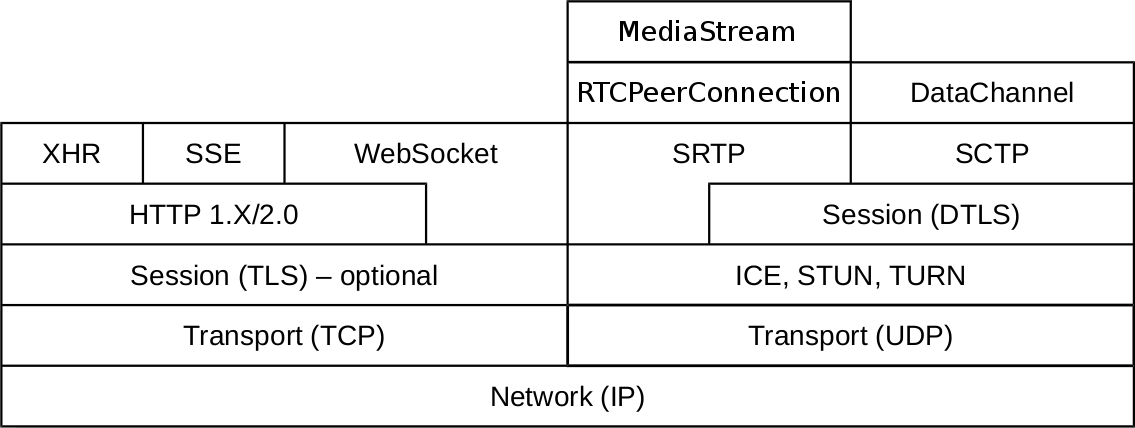
\includegraphics[width=0.8\textwidth]{figures/webrtc_stack.png}
	\caption{WebRTC protocol Stack}
\end{figure}

\ac{WebRTC} defines three main \ac{API}s: MediaStream, PeerConnection and DataChannel. 

\begin{itemize}
  \item \textbf{MediaStream} allows the browser to access the camera, microphone and the device's screen. 

  \item \textbf{PeerConnection} acquires connection data and negotiates with peers.
%RP establishes and negociates a connection with a peer for transmitting real-time video or audio?
  \item \textbf{DataChannel} provides a channel for exchanging arbitrary data with other peers.
\end{itemize}

\ac{WebRTC} uses \ac{UDP} for transporting data, which provides lower latencies than \ac{TCP}, but is not reliable and does not assure packet order and integrity. \ac{SCTP} and \ac{SRTP} are used for streaming data, providing a mechanism for congestion control and partial reliable delivery over \ac{UDP}. All transferred audio, data and video must be encrypted with \ac{DTLS} symmetric keys. \ac{DTLS} provides the same security guarantees as \ac{TLS}. 

\ac{TLS} doesn't support independent packet decryption\cite{rfc6347}, for that it requires a reliable transport channel, typically \ac{TCP}. The decryption of a packet depends on the previous packet, which for unreliable transport protocols like \ac{UDP} may represent a problem, either due to packet loss or different reception order.

\ac{DTLS} is similar to \ac{TLS}, but is used on top of \ac{UDP}.
The main difference is the inclusion of a sequence number per packet that is used for packet re-ordering on reception and protects from duplicated packets. If a packet sequence number is less than the expected sequence number the packet is discarded. If a packet sequence number is greater than the expected sequence number the packet may be enqueued or discarded. By knowing the sequence of messages that are sent and received in \ac{DTLS}, timers are used for packet retransmission avoiding acknowledgment messages.
%RP TLS?

\begin{figure}[H]
	\centering
	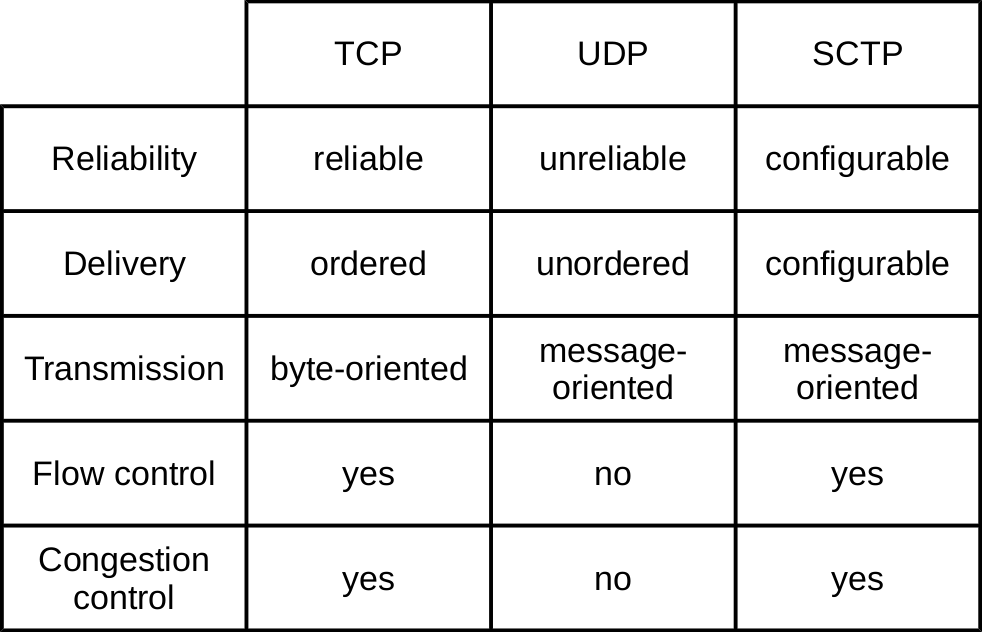
\includegraphics[width=0.6\textwidth]{figures/basic_protocols.png}
	\caption{Overview of transport protocols}
\end{figure}

\ac{WebRTC}'s \emph{DataChannel} is built on top of \ac{SCTP}, which is encapsulated by \ac{DTLS}. \ac{DTLS} encapsulation provides confidentiality, authentication and integrity to the transfered data. A \emph{Data Channel} has one incoming stream and one outgoing stream, providing bidirectional communication. Each data channel direction can be configured for reliable or unreliable transmission, the same can be done for order delivery and priority. which can also be defined for improving the quality of service of a particular stream over the others.

\ac{WebRTC}'s \emph{MediaStream} is built on top of \ac{SRTP}, which requires an external mechanism for key exchange. \ac{DTLS} keys are negotiated on handshake in order to achieve a secure connection. The new keys derived from \ac{DTLS} handshake are seized for \ac{SRTP} encryption, the remaining \ac{SRTP} communications are done through \ac{UDP} without using \ac{DTLS}.
%RP quais remaining?  A última frase é confusa

\ac{WebRTC} aims to provide a standard platform for real-time audio and video on the Web. It arrives at a time when several proprietary products are well established.
\emph{Skype}\footnote{\url{http://www.skype.com/}(accessed June 1, 2015).} is an application that allows video, voice, instant messaging and multi-party communication over proprietary protocols, its main strength are the amount of users that are using it nowadays and the ability to perform voice calls to the \ac{PSTN}. But compared to \emph{Skype}, \ac{WebRTC} applications don't need to be pre-installed.

\emph{Google Hangouts}\footnote{\url{http://plus.google.com/hangouts}(accessed June 1, 2015).} is another popular video multi-party conference web application. 
In the past, in order to use \emph{hangouts} on a web browser a plug-in had to be installed, nowadays hangouts is using \ac{WebRTC}. \emph{Google Hangouts} supports viewing videos on \emph{youtube} synchronously, drawing collaboratively, creating music and playing multi-player games. These applications are implemented with \emph{Adobe Flash}.  

\emph{Jitsi Meet}\footnote{\url{http://jitsi.org/Projects/JitsiMeet}(accessed June 1, 2015).} is a \ac{WebRTC} collaborative application that uses \emph{Jitsi Videobridge} for high quality and scalable video conferences and supports shared document editing. \emph{Jitsi Meet} allows a great amount of users in the same conversation by identifying the current most active participant users and, by consequence, reducing the video and audio quality for all the other users. \emph{Jitsi Videobridge} is a server that enables multi-party video calls. 

%RP a descricção do skype, hangouts e jistsi cai um pouco do céu. Não há uma transição e não é feita uma análise. Apenas são indicados. Não há comparação entre eles nem com o que pode ser feito por webrtc.



\section{Signaling: meet and get to know}
\label{signaling}


  Signaling is the process by which applications exchange connection information about peers and servers, their capabilities and meta-data.
  In particular, \ac{WebRTC} does not implement signaling, as different applications may require different protocols and there is no single answer that fits all problems.
  As a consequence, multiple options are available for filling the missing \ac{WebRTC}'s signaling component, which can be performed using \ac{SIP}, \ac{XMPP}, \emph{WebSockets}, \emph{Socket.io}\footnote{\url{http://socket.io/}(accessed June 1, 2015).} or by implementing a custom protocol.

  \subsection{WebRTC}

  \ac{WebRTC} uses \ac{SDP}~\cite{rfc4566} to define peer connection properties such as types of supported media, \emph{codecs}, protocols used and network information. An \ac{SDP} offer describes to other peers the expected type of communication and its details, such as used transport protocols, codecs, security and other.

  One of \ac{WebRTC} signaling's requisites is bi-directional communication.
%RP acrescentei o webrtc pois isto não é um requisito geral de signaling. era o que querias dizer?
%HR sim é isso
  \ac{HTTP} uses a request-response paradigm, where a request is sent by the client, followed by a server response.
  %in other words, it follows an unidirectional communication.
%RP de certeza que queres dizer que o http é unidirecional? 
%HR era mais o facto de o servidor não poder comunicar com o cliente sem que o cliente comunique primeiro (tem que haver uma iniciativa por parte do cliente)
  Sometimes it is required that some information be obtained in real time, but we saw, some \ac{NAT}'s do not support callbacks from servers, preventing them from notifying clients as soon as an event occures.
One technique to overcome this problem is polling. Polling consists on sending periodic messages to which the server responds immediately with empty content or fresh information. Text and presence messages are unpredictable, if the time between periodic requests is short, most of the time the server will return empty results wasting network bandwidth and energy. On the other hand, if the time between periodic requests is large, newer messages may arrive too late.
%RP  Real time communications are unpredictable. Normalmente falamos de audio e video, que são previsíveis. Estás a referir-te às comunicações em si ou ao signaling e estabelecimento?

A technique called long polling consists on making the server hold the request until there is fresh information or expiring it after some time.
As soon as it receives the reply, the client makes another request. Long polling technique results on a better network usage and a faster server response, but both simple polling and long polling requests are sent with \ac{HTTP} headers, which add data overhead and can be noticed especially for short sized messages.

The \emph{WebSocket} protocol allows bi-directional communications over a full-duplex socket channel~\cite{rfc6455}, by other words it supports sending and receiving data simultaneously.
%RP coloca as citações no final da frase. Pode haver excepções onde a citação apenas cobre parte da frase ou precisas de colocar várias a dizer coisas diferentes.
 \emph{WebSocket} handshake phase specifies a \ac{HTTP} header in order to upgrade to \emph{WebSocket} type of communication, but the remainder messages are exchanged without \ac{HTTP} headers, which leads to much smaller messages and better network usage. WebSockets may not be available on every web browser, frameworks like \emph{socket.io} and \emph{SockJS}\footnote{\url{http://github.com/sockjs}(accessed June 1, 2015).} fall back to using \ac{HTTP} long polling when there is no support for \emph{WebSockets}. 

  \ac{BOSH}~\cite{xep0124} is a technique based on long polling that uses two socket connections and allows sending client messages to the server while a previous request is held.
  The \ac{BOSH} specification assumes that a connection manager is implemented to handle \ac{HTTP} connections. This connection manager is basically a translator from \ac{HTTP} to raw message so that the server may be implemented as if this communication is performed over \ac{TCP}.
  When the connection manager holds for a response for too long, it responds with an empty body, this technique prevents an \ac{HTTP} session from expiring when the client is waiting for a response, thus expanding the session time. Expiring sessions can be expensive due to the overhead of establishing new connections, which is even worse when \ac{HTTP} is used over \ac{SSL}.

  If the server is holding a request, it maintains a second connection to receive more requests from the same client. The request on hold returns immediately with a possible empty body leaving its socket free, while the second connection serves the polling loop. The exchange of roles of those two connections allow to pull data from multiple contexts instead of being locked in just one.
  %RP estas duas frases dizem o mesmo da perspectiva do cliente e do servidor. Não consegues simplificar numa só?

  \subsection{Session Initiation Protocol}

  \ac{SIP}~\cite{rfc3261} is a protocol used for negotiation, creation, modification and finalization of communication sessions between users. \ac{SIP} follows a client/server architecture with \ac{HTTP} like messages and it can be used as a signaling protocol. The advantage of \ac{SIP} is the ability to make video and voice calls between the telephone network and applications over \ac{IP} networks.

  The working group \ac{SIMPLE}\footnote{\url{https://datatracker.ietf.org/wg/simple/documents/}(accessed June 1, 2015).} proposed the creation of \ac{SIP} extensions, namely presence information~\cite{rfc5263} and instant messaging~\cite{rfc3428}.

  \ac{SIP} is used in \ac{VoIP} applications due to its compatibility with the \ac{PSTN}.
  Service providers are making their \ac{SIP} infrastructures available through WebSockets\footnote{\url{https://tools.ietf.org/html/draft-ietf-sipcore-sip-websocket-10} (accessed March 25, 2016)}.
%RP a frase anterior é estranha
  Frameworks like \emph{jsSIP}\footnote{\url{http://jssip.net/}(accessed June 1, 2015).}, \emph{QoffeeSIP}\footnote{\url{http://qoffeesip.quobis.com/}(accessed June 1, 2015).} and \emph{sipML5}\footnote{\url{http://sipml5.org/}(accessed June 1, 2015).} are used on the client side to parse and encode \ac{SIP} messages, making \ac{SIP} accessible to web based applications. 
%RP quando usas footnotes para indicar sites deves acrescentar ``last accessed (data)''. Isto é importante pois os sites são documentos efémeros que podem dizer uma coisa diferente mais tarde.
  \ac{SIP} with \emph{WebSockets} can be used as a signaling method for \ac{WebRTC} applications, it allows web browsers to have audio, video and \ac{SMS} capabilities like mobile phones. For instance, it is possible to inter-operate web communications with \ac{SIP} networks, mobile and fixed phones.

\subsection{Extensible Messaging and Presence Protocol}

  \ac{XMPP} was initially developed for instant messaging and presence (Jabber\footnote{\url{http://jabber.org/}(accessed June 1, 2015).}). It is nowadays an open technology for standardized, decentralized, secure and extensible real-time communications. 
  \ac{XMPP} messages are \ac{XML} based, which is attractive for applications that need structured messages and rich hypermedia. Another advantage of \ac{XMPP} is the addition of extensions, for example \emph{XEP-0096}~\cite{xep0096}, which adds file transfer capabilities between two entities, and \emph{XEP-0045}~\cite{xep0045}, which enables multi-user chat.
  \ac{XMPP}'s bi-directional communication over \ac{HTTP} is achieved through \ac{BOSH}~\cite{xep0206}.
  This kind of communication is also possible through WebSockets~\cite{rfc7395}.
  Today, multiple \ac{XMPP} server implementations exists, such as: \emph{ejabberd}\footnote{\url{http://jabberd.im/}(accessed June 1, 2015).}, \emph{Metronome}\footnote{\url{http://lightwitch.org/metronome}(accessed June 1, 2015).}, \emph{Openfire}\footnote{\url{http://igniterealtime.org/projects/openfire/}(accessed June 1, 2015).} and \emph{Prosody}\footnote{\url{http://prosody.im/}(accessed June 1, 2015).}. \emph{Ejabberd} is the server that implements more \ac{RFC} specifications and \ac{XEP}s\footnote{\url{http://en.wikipedia.org/wiki/Comparison_of_XMPP_server_software}(accessed June 1, 2015).}.
  %RP fazes muitos paragrafos. Um paragrafo por tecnologia é normalmente suficiente se não forem muito grandes.
  

    One of the advantages that \ac{XMPP} based applications offer is the possibility to send messages across different servers. An \ac{XMPP} user is identified by its \textit{Jabber ID}, which is defined by the pair username and server name in the form \textit{username@server}.

    The user profile is represented in terms of Data Forms~\cite{xep0004} protocol and managed (registration and update) through \textit{Info/Query} (IQ)~\cite{rfc3920} requests to the \ac{XMPP} server, which responds with an IQ response containing information to retrieve the registration fields needed to fill its profile (eg username, password, telephone). 
%RP frase demasiado longa. Torna-se confusa.
    
    An important aspect of this model is the ability to define a user as a set of attributes that can change dynamically in order to fit the \ac{IM} application's needs. 

    The connection to the \ac{XMPP} server can be done through the same web server as the user is connected, but this web server would handle a lot of connections and that would have a great impact on the overall system performance. On the other hand, users can directly connect directly to \ac{XMPP} servers from web applications using the \emph{JavaScript} library \emph{strophe.js} \footnote{\url{http://strophe.im/strophejs/} (accessed May 6, 2016).}

    Typically a web application consists in multiple web pages which are navigated by users. Each time a web page is accessed, either from a new context or a transition from a previous page, its context is cleared except for local storage and cookies. The \emph{JavaScript} context is cleared, including the \ac{XMPP} connections performed by \emph{strophe.js}. As such, an automatic mechanism is required for avoiding the implicit user reauthentication.
    One solution for reauthentication can be achieved by storing the user's JabberID and password on local storage and every time a page is accessed the authentication is performed without the users knowledge. Clearly this solution represents security flaws as the local storage can be easily accessed locally or by performing a cross site scripting attack to reveal all the local storage. The same problem arises if the credentials are stored on cookies.
    %RP tinhas este comentário (HOW? explain!)
    %RP o strophe.js caiu aqui da paraquedas! Explicar o que é

    An alternative solution is known as Session Attachment \footnote{\url{https://metajack.im/2008/10/03/getting-attached-to-strophe/} (accessed May 6, 2016).}, which requires that a \textit{session identifier}(SID) together with a \textit{initial request identifier (RID)} be passed to \emph{strophe.js} in order to re-connect to the same stream on \ac{XMPP} server. Either SID and RID are unpredictable and, particularly, \textit{RID} changes on every request making it worthless if a user maintains more than one tab opened, for example for multiple conversations at the same time.
    %RP either ou both?
    %RP verifica se não alterei o sentido da frase
    
    Another alternative would be the development of our solution in a single web page, which would increase drastically the complexity of our web application.

    We know that an \ac{XMPP} based application could simplify our work just by using functionalities that \ac{XMPP} already implement, but  we do not need all of them. In fact, we just need a subset of \ac{XMPP} features, namely a simple way to register users, access and edit user's information, create chat rooms, send messages and access to presence information.


  \subsection{Signaling-On-the-fly}


  Another interesting approach for signaling would be \ac{SigOfly} which allows inter-domain real-time communications, while abstracting the protocol used~\cite{sigofly}.
%RP o ~ antes do cite faz com que não haja um espaço mas não haja uma mudança de linha entre a última palavra e a citação
  \ac{SigOfly} provides inter-domain communication by making use of the \emph{Identity Providers} of each peer. 
  The caller entity downloads a page with all the code needed, also known as messaging stub, to communicate with the called party.
  This code contains an implementation of the signaling protocol used in order to communicate to the called peer. If the called party domain is being overused, it is possible to switch the caller and called parties role, after that the called entity downloads the stub code from the caller domain instead.
  \ac{SigOfly} is an approach very flexible because participants on a video call are not tied to just one type of signaling implementation. Another important aspect of \ac{SigOfly} is the ability to perform multi-party conversations either through a \emph{Mesh Topology} or a \emph{Multipoint Control Unit}.
%RP os outros não permitem multi-party?
%HR adicionei ao Hangouts e Skype, quanto ao XMPP já digo que existe uma extensão que permite multi-user chat

\section{Hypermedia: more than words, more than images}
\label{hypermedia}

Since the early days of video technology, one of the problems raised consisted on how to add more information onto video without generating multiple versions. This section examines technologies that allows different ways to present multimedia content in such a way that it change based on synchronization amongst other multimedia elements or user interaction.

\emph{Hypertext} is a type of text that provides links to texts or other types of content, these links are known by \emph{hyperlinks}. \emph{Hypermedia} is an evolution of \emph{hypertext}, it includes audio, images, text and video. 

\emph{Hypermedia} concept brings the possibility to organize and overlay multimedia elements into a nonlinear linear structure.

In the beginning of analog video technology, the navigation over it was quite limited to simple operations such as play, stop, rewind and fast-forward. As video started to be digitalized, new operations over video emerged, such as random jumps and chapter navigation through interactive menus present on \ac{DVD}.

%RP depois disto falta uma introdução a explicar que precisas de controlar a apresentação e execução de diversos conteúdos e que para isso vais precisar de uma tecnologia que permite sincronizar e controlar. Esta secção examina isso.

Some \ac{MPEG} implementations, like \cite{embedded}, added hypermedia information to empty space present on \ac{MPEG} frames in order to provide interactive television, modifying the \ac{MPEG} encoder and decoder in order to handle hypermedia content.
%RP esta última frase, com detalhes de implementação fica algo deslocada antes de apresentares os exemplos de hypermedia. Talvez deslocar para mais tarde.
Hypermedia is a concept that holds the promise of future technology and features but it is also already present in our daily lives.
%RP por exemplo na publicidade no youtube

  Subtitles are an example of information that might be required.
  The need to translate movies, raised the problem whether it is appropriate to change the original video or audio. For example, subtitles should be an entity independent from the video, in order to be personalized or replaced easily.

  \ac{SAMI}, and \ac{SRT} are two of the multiple formats for subtitles commonly supported by video players. Although those formats have styling available, they are quite limited to text. 

  Hyper-video is a kind of video that contains links to any kind of hypermedia, including links to skip part of it. An example of hypermedia application could be a search engine over hypermedia content, like subtitles, in order to jump to a specific time in a video or audio track. \emph{HyperCafe} \cite{hypercafe} was an experimental project to expose hyper-video concepts that consisted of an interactive film that enabled switching between different conversations taking place inside a cafe.
 
  Detail-on-demand is a subset of hyper-video that allow us to obtain additional information about something that appears along the video, like obtaining information about a painting that appears in a particular segment. \emph{Hyper-Hitchcock}\cite{hitchcock} is an editor and player of detail-on-demand video.

  In order to navigate through a dynamic video, we must be aware of time synchronization and the multiple time flows, it ils important that all time, causality and behavior rules are well defined.
  %RP one must be aware? O utilizador? Ou queres dizer que é preciso definir as relações? O que falas a seguir é sobre linguagens para isso.
  
  \emph{HyVAL}\cite{hyval} is an \ac{XML} based language that was proposed for modeling composition, synchronization and interaction of hypermedia. HyVAL defines defines video structure, internal video and external media objects. 
  \emph{HyVAL} uses a primary video stream, around which all other elements are organized and synchronized.
  \emph{HyVAL}'s video structure object defines a structure derived from traditional video, which divides video into segments, scenes, shots and frames hierarchically. 
  This approach is quite restrictive if we want to apply hyper-video concepts to videos that don't follow this structure. External media objects are linked by primary video, those objects can represent other videos, images, text, animation and sound.
  %RP não percebo bem a última frase. O que é primary video?

  \ac{SMIL}\cite{smil} was introduced to describe temporal behavior of multimedia content, in particular, it could be used to overlay subtitles on films. With \ac{SMIL} it is possible to synchronize multiple videos, either in parallel or in sequence, reproduce a different audio track, overlay user interface elements with hyper-links, among multiple other features.
  %RP synchronize multiple sections of video? vários videos apresentados em simultâneo?

  \ac{SMIL} is an \ac{XML} based language that defines twelve modules: \emph{Animation}, \emph{Content Control}, \emph{Layout}, \emph{Linking}, \emph{Media Objects}, \emph{SmilText}, \emph{Meta Information}, \emph{Structure}, \emph{Timing}, \emph{Time Manipulations}, \emph{State} and \emph{Transitions}.


\begin{itemize}

  \item The \textbf{Animation} module contains elements and attributes that define a time based mechanism for composing the effects of animations. For example, this module can perform changes on \ac{XML} or \ac{CSS} attributes like color and dimensions.  

  \item The \textbf{Content Control} module contains elements and attributes that provide optimized alternatives for content delivery. For example, it could be used to change audio language in function of user's nationality, for videos with multiple audio channels.

  \item The \textbf{Layout} module contains elements and attributes for coloring and positioning media content. Other layout mechanisms are also possible, such as \ac{CSS}.

  \item The\textbf{Linking} module contains elements and attributes for navigational \emph{hyperlinking}. Navigation can be triggered by events or user interaction.

  \item The \textbf{Media Object} module contains elements and attributes for referencing rendering behavior of external multimedia or control objects.

  \item The \textbf{SmilText} module contains elements and attributes that define and control timed text. For example, this module could be used to create labels and captions.

  \item The \textbf{Meta Information} module contains elements and attributes that allows describing the \ac{SMIL} document. For example, this module could be used to define movie details such as category, director, writers and cast.

  \item The \textbf{Structure} module defines the basic elements and attributes for structuring \ac{SMIL} content. This module defines a \emph{head} element that contains non temporal behavior information defined by  \emph{Meta Information}, \emph{Layout} and \emph{Content Control} modules. This module also defines the \emph{body} element, where all temporal related module information is contained.

  \item The \textbf{Timing} module is the most important module on \ac{SMIL} specification. Due to its complexity, it is divided into seventeen sub-modules for coordination and synchronization of media over time. The three main elements are \emph{seq}, \emph{excl} and \emph{par}, that, respectively, play child elements in sequence, one at a time and all at the same time. 

  \item The \textbf{Time Manipulations} module adds time behavior attributes to \ac{SMIL} elements, such as speed, rate or time.

  \item The \textbf{State} module defines attributes that define the state of \ac{SMIL} elements, such as element visibility, current element time, amount of repeated loops, playing state and many others.

  \item The \textbf{Transitions} module defines attributes and elements for transitions across multiple \ac{SMIL} elements according to the \emph{Timing} module.

\end{itemize}

The \ac{DOM} is a standard \ac{API} that allows easy management of documents that are organized in a tree structure, by providing \ac{CRUD} operations over its elements and their attributes. \ac{DOM} makes it easy to inter-operate between imperative and declarative programming languages\cite{dom}.
%RP não arranjas uma referência para o dom?

Like \ac{DOM}, \ac{SMIL} \ac{DOM} is an \ac{API} for \ac{SMIL} documents. Allowing \ac{CRUD} operations over \ac{SMIL} documents is an important feature for extending \ac{SMIL} capabilities, for example for creating non-linear animations and triggering external events like \emph{JavaScript} functions.  


  \ac{SMIL}'s modules can be used to synchronize and animate \ac{XHTML} and \ac{SVG} elements.
  %RP ``are used'' ou ``can be used''?
  
  \ac{SMIL} fits our goals for creating a multimedia rich hyper-call, but it lacks on browser compatibility. Ambulant \cite{ambulant} was one of the SMIL players that were developed for browsers, although this player implements most of \ac{SMIL} 3.0 \cite{smil3} specifications, it needs to be installed on browsers as a plug-in.

  SmillingWeb \cite{smillingweb} attempts to implement a cross platform multimedia player designed for \ac{SMIL} 3.0 presentations with \emph{JavaScript} and \emph{jQuery} which, unlike \cite{ambulant}, doesn't require a plug-in to be installed and shouldn't have incompatibility issues. 
  SmillingWeb already takes advantage of \ac{HTML}5 and \ac{CSS}3.
  It takes into account unsupported web browsers through the use of \emph{Modernizr}\footnote{\url{http://modernizr.com/}(accessed June 2, 2015).}, a simple \emph{JavaScript} library that may require plug-ins if new features aren't supported.  
  But SmillingWeb just implements a subset of \ac{SMIL} 3.0 and their scheduler engine loads the \ac{SMIL} file only once, which could raise problems when dealing with \ac{SMIL} changes due to real time communications.
  Another problem with SmillingWeb is pre-loading and playing elements at the correct interval of time, which is not always possible due to high latency networks leading to  pauses during playback.

% XXX
  %RP fazes uma mudanças de tema muito bruscas. Podes usar \subsubsection ou \paragraph para dividir isto melhor. E uma frase entre temas a servir de ``cola'' ou ``separação'' também não fica mal


  An alternative to \ac{SMIL}'s \emph{Layout} module is to use \ac{HTML} which is a markup language based on \ac{XML} that is used for creating web pages. \ac{HTML} alone is a very poor language when we are focused on visual appealing and interactive web pages. Languages like \ac{CSS} and \emph{JavaScript} are typically used along with \ac{HTML} for improving the interaction and appearance of a web page. 


  %RP esta parte está um pouco confusa. Primeiro falas de smil, depois de html, depois de smil novamente. Devias agrupar tudo. Devias agrupar as soluçoes por tecnologia. Se preciso, primeiro fala de html, css, etc, e depois de smil e das implementação de smil (incluindo as que são implementadas em html e js).
  
  \ac{CSS}'s goal is to separate the structure of an \ac{XML} document from its appearance. \ac{CSS} defines styles for \ac{XML} tags based on their name, class, identifier or position.
  Besides static styling \ac{CSS} also supports animation and transitions leading to more dynamic content.
  %RP Tens muitas alturas em que não começas frases novas. Usas virgulas para separar conteúdo que não faz sentido ficar na mesma frase pois começa com um novo sujeito seguido de verbo.

  \emph{JavaScript} is an imperative object-oriented language based on \emph{ECMAScript}. It is used mainly on client-side and executed by a web browser. \emph{JavaScript} has its own implementation of \ac{DOM} and one of its advantages is the ability to download and execute code on the fly without the need of pre-installed plug-ins.

  \emph{JavaScript} has compatibility issues among the different web browsers, leading to different behaviors. To solve that problem, there are libraries written in \emph{JavasSript}, namely \emph{jQuery}, that implements the same functionality for multiple browsers, masking most of the incompatibility issues.

  With the emergence of \ac{HTML}5, tags like \emph{video}, \emph{audio} and \emph{track} allow us to play video with multiple \emph{codecs}, audio and subtitles in \ac{WebVTT} format. Another important tag is \emph{canvas} that allows drawing graphics with \emph{JavaScript} on a rectangle within a web page.

  For example, with \ac{API}s like WebGL\footnote{\url{http://khronos.org/webgl/}(accessed June 2, 2015).}, it is now possible to manipulate a three dimensional environment in the context of a hyper-call. Another example would be a collaborative spreadsheet using \ac{WebRTC}. With this, hyper-calls are not limited to only audio, image, text and video, but also interaction with complex graphical user interfaces that changes over time.


  \ac{SVG} is an \ac{XML} based format that incorporates the animation module of \ac{SMIL}. Currently, \ac{SVG} allows adding movement and animating attributes of elements. When embedded on \ac{HTML}5, it allows dynamic changes to inner content in real-time through the \ac{DOM} \ac{API}. Besides that, it also allows calling \emph{JavaScript} functions on events such as animation end, mouse over and mouse click.
  
  Back in 1995, \emph{flash}\footnote{\url{http://www.adobe.com/products/flash.html}(accessed June 2, 2015).} was developed for web-based animations. Introducing video support in 2002, \emph{flash} started to grow after that. Competitor's players, at that time were focused on playing video and audio, while \emph{flash} had vector graphics and focused on streaming \emph{on-demand} video across multiple platforms. \emph{VP6} was their choice of video \emph{codec}, providing half the video size (in Byte) for the same quality and providing video quality adjusted to \emph{Internet} connection latency. 
  In 2010, \emph{Adobe Flash} was the most widely used applications for reproducing live broadcast and recorded video \cite{flashvideo}, it supports progressive video download using \ac{HTTP} and streaming using \ac{RTMP}.

  \ac{RTMP} is a \ac{TCP} based protocol used for streaming audio, video and data between a \ac{FMS} and \emph{flash} players. A bidirectional connection is established between the two in order to allow real time communications. A \emph{flash} player can stream a webcam video to a \ac{FMS} using \ac{RTMP} or it can request a video stream to \ac{FMS} that can either be a pre-recorded stream, live stream or data. Multiple \ac{FMS} servers can be used in parallel to increase capacity and handle more streams simultaneously.
  %RP chained ou usados em paralelo?

  \ac{FMS} can stream video and audio to one or more subscribers by sending a separate copy for each subscriber. With \ac{RTMFP} it is possible to stream video directly between \emph{flash} players, allowing a publisher to break up a stream into pieces that can be cooperatively distributed in a P2P mesh. \ac{RTMFP} uses \ac{UDP} to speed packet delivery, which although it is not reliable, is well suited for video streaming. Like \ac{WebRTC}, \emph{flash} players also need to apply techniques like \ac{STUN} and \ac{TURN} for \ac{NAT} traversal.

  Although \ac{HTML}5, \emph{JavaScript}, \ac{CSS} and \ac{WebRTC} implement some of \emph{flash}'s features, it doesn't mean that \emph{flash} will be replaced soon.
  Instead, both technologies can be used to develop rich \emph{Internet} applications.
  It is also important to note that \ac{HTML}5 is better supported in mobile devices than \emph{Adobe Flash}. 

  Like \emph{Flash}, \emph{Microsoft Silverlight}\footnote{\url{http://www.microsoft.com/silverlight/}(accessed June 2, 2015).} is a cross browser plug-in and platform that is used to develop rich \emph{Internet} applications. It supports vector graphics, animation and video. Compared to \emph{flash}, which uses \emph{ActionScript}, \emph{Silverlight} applications can use languages like C\#, \emph{VisualBasic} and \ac{XAML}. \emph{Silverlight} uses a technique called \emph{Smooth Streaming} from \emph{IIS Media Service} that consists on delivering video in real-time with adjusted quality in function of bandwidth variations and \ac{CPU} usage.

  Using technologies that relies only on web standards, like \ac{CSS}, \ac{HTML}5, \emph{JavaScript} and \ac{SVG}, will make possible to develop an application that solves our problem with the advantage of being compatible with a greater amount of web browsers.
  %RP não concordo com frase. O que o uso de tecnologias standard faz é garantir que a app é suportada em vários dispositivos. Também podes dizer as essas tecnologias já permitem desenvolver a applicação que tens em mente, mas isso é outra coisa.
  %RP evita ser tão ``vendedor''. Não digas coisas como ``to a new level'' mas cinge-te a afirmaçãos objectivas.


  %In this project our goal is to enrich hyper-calls with no limits, every user should be free to choose how it wants to be contacted and how he wants to share its contents.
  %RP O ``no limits'' é muito vago. Tens de ser mais objectivo.
  %HR tanto esta como a seguinte frase foram escritas praticamente no inicio do estado de arte, nem faz sentido estarem aqui. 

  %In order to give users a personalized communication channel, each user must have a personal web page where its available plug-ins could be downloaded from other peers, after that, they can talk in the same language whatever it is.
%RP acho que aqui já estás a falar de detalhes de implementação que o leitor não tem possibilidade de perceber antes de descreveres as funcionalidades de aplicação e a sua arquitectura.



\section{Extending collaboration tools with time manipulation}
\label{collab}

Real time collaboration applications have become a huge help on team tasks, providing a great boost on business, research and investigation velocity. Technologies like these are appearing along these days, but they were not be possible a few years ago because technology was limited or unavailable. Although today's technology is still limited on some aspects, progress is being done in order to improve the web ecosystem, by creating standards and migrating to newer technologies.
%RP aqui dizes ``we are doing progress''. Parece que é parte do teu trabalho e que tens algo a ver com isso. Muda para frase impessoal

Section \ref{recstream} presents the RTP protocol how it can be used to record media streams. Section \ref{mediatype} describes the media types and what types of media should be streamed. Section\ref{intrecord} addresses how an interactive media can be recorded. Section \ref{collabenv} presents the collaborative environment and libraries to synchronize distributed object among users.

\subsection{Streaming and Recording}\label{recstream}~\\
	If, for instance, one wants to rewind a real-time video, recordings will be needed from whom is streaming the video. 
 Our first concern on real time collaboration applications, besides the communication itself, is the data storage and representation. Storing multimedia content is not a viable solution because most browsers recommend limiting local storage to at most five megabytes per origin.

 	In order to provide a way to record and playback streams, additional servers will be required to process and record the large amount of data generated by audio and video streaming.

 \ac{RTP}\cite{rfc3550} is used for streaming audio and video over \ac{IP}.
 Multimedia content is transported on the payload of \ac{RTP} messages, that contain headers for payload identification. \ac{RTP} is independent from its payload type, allowing it to transport any kind of encoded multimedia. A sequence number is used for sorting received packets.

\ac{RTCP} is used for controlling \ac{RTP} multimedia streams, it provides bandwidth statistics and control information that can be used for changing the quality of the stream in real-time.

  \ac{RTP} allows to change its requirements and add extensions to it with profiles. One of the most used ones is the \ac{RTP} profile for audio and video \cite{rfc3551}, which lists the payload encoding and compression algorithms. This profile also assigns a name to each encoding which may be used with other protocols like \ac{SDP}.
  Another profile for \ac{RTP} is defined by \ac{SRTP}, which provides encryption, authentication and replay protection for \ac {RTP} traffic. The analogous secure protocol for \ac{RTCP} is \ac{SRTCP}.

  Both \ac{SRTP} and \ac{SRTCP} use \ac{AES} by default, which is a symmetric-key algorithm for data encryption. Each packet is encrypted using a distinct key-stream, as otherwise, using a single key-stream with \ac{AES} on \ac{CBC} would make it impossible to recover from packet loss.

  Two key-stream generators for \ac{AES} were defined: \emph{Segmented Integer Counter Mode} and \emph{f8-mode}. If a packet is lost, there is no impact on other packets, as the initialization vector is obtained through those key-stream generators and it is fixed for each packet.
  %RP isto está tudo no RFC3550? Se não, faltam muitas citações.
  %HR esse RFC é grande


  \ac{RTP} recorders are independent of payload encoding, they don't decode \ac{RTP} packets, they record packets instead, allowing to record all video and audio formats even if they're encrypted.

        %RP lá vais tu mudar de tema da conversa sem explicar porquê....
        Even though one on one calls are common, there are occasions when several people take part of the same video call.
	Multi-party video calls can be achieved on \ac{WebRTC} by streaming video from each participant to all the other participants. Although this works, the bigger a conference room is, the bigger is the bandwidth used to stream video to all participants within the conference room.
        In this scenario, a more efficient alternative to peer-to-peer is the use of a \ac{MCU}.

	\emph{Jitsi Video Bridge} \footnote{\url{http://jitsi.org/Projects/JitsiVideobridge}(accessed June 2, 2015).} receives one stream from every participant on a conference, either from a \emph{jitsi} client or a \emph{WebRTC} application, and redirects it to all the other conference participants, reducing the amount of data that each peer sends. Although all the participants still need to download all the streams from the \emph{Jitsi Video Bridge} server, typically download rates are much bigger than upload rates, making this solution more feasible.
	\emph{Jitsi Video Bridge} uses \ac{XMPP} as a signaling protocol and its \emph{colibri} extension \cite{xep0340} to reserve channels for video transmission. Despite this choice for signaling protocol, \emph{Jitsi Video Bridge} also supports \ac{SIP}.

	{\color{blue}
	\ac{KMS} supports trans-coding, group communications, recording, mixing, broadcasting, applying filters, image and sound analysis, for example it allows face and qrcode detection. \ac{KMS} functionalities are exposed through \emph{JSON-RPC} over \emph{WebSocket}, there are three clients available: \emph{JavaScript} client for web browsers, \emph{Java} client for \emph{Java EE} servers and \emph{JavaScript} client for \emph{Node.js} servers. 
	\ac{KMS} supports streaming over \emph{WebRTC}, \ac{HTTP} and \ac{RTP} endpoints. Another important component of \ac{KMS} is \emph{Kurento Repository} which supports recording and playing directly from \emph{MongoDB}, that is important for providing a scalable media storage. Unlinke \emph{Jitsi Video Bridge}, \ac{KMS} does not enforce a specific signaling protocol.
	}

\subsection{Media Types}\label{mediatype}~\\
	Media Types can be distinguished by two criteria, the first one describes a media as discrete or continuous, the second one describes it as interactive or non-interactive. A discrete media is characterized by not depending from time, and continuous media as depending on it. Interactive media is characterized by its state being changed by external events such as user interactions.
  %RP estavas a falar de gravar video e passaste a falar de protocolos de streaming. Convém explicar o racional para esta abordagem. Começa a secção a explicar sobre o que vais falar e porquê.
  %RP e usa subsecções...
\begin{figure}[H]
	\centering
	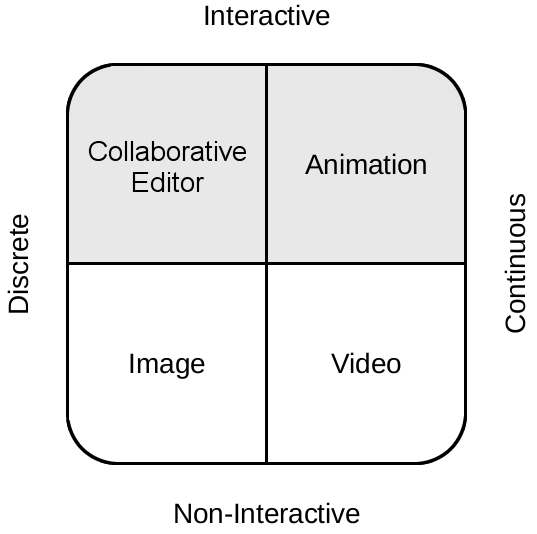
\includegraphics[width=0.4\textwidth]{figures/media_types.png}
	\caption{Media Types}
\end{figure}
	For example, an image is non-interactive and discrete, while a video is continuous and non-interactive. A simple collaborative editor with just text is interactive and discrete. An animation that changes in function of user behavior is interactive and continuous.

	Streaming protocols like \ac {RTP} and \ac{RTSP} were designed for continuous and non-interactive media types, such as audio and video. Discrete and non-interactive media don't need to be streamed through \ac{RTP} because they don't change with time. For example, if an image appears in a specific time interval, just the \ac{HTML} or \emph{JavaScript} that will reference the image must be streamed, the image itself is then transferred through \ac{HTTP}.

	In order to play a stream, a player must be prepared to interpret the stream content. For interactive stream the player must download an environment, decode the \ac{RTP} payload to determine the state and display it to the user. Streaming interactive media like a combination of \ac{HTML}, \ac{CSS} and JavaScript requires more than interpreting the code: a streamed user interface may contain an internal state that is not shown on code.
        %RP não percebi
        

 \subsection{Recording and Streaming Interactive Media}\label{intrecord}~\\
    Mauve et al. proposed an \ac{RTP} profile for real-time transmission of interactive media\cite{interactive_stream}. This new profile reuses much of video and audio profile implementation, integrating the interactive component. Hilt et al. explained how to record interactive video with this new profile \cite{interactive_record}.
        %RP não uses a citação como sujetio das frases. O trabalho não tem um nome?

	Every time an event is processed on one of the endpoints, both sender and receivers state must stay synchronized, otherwise events may behave differently.
	To achieve synchronization of interactive data, most packets have three types: \emph{State}, \emph{Delta-State} and \emph{Event}. State packet defines the environment complete state. Delta-State packets transports just the piece of state that changed. Event packets informs that an event occurred over the interactive media. 
%RP referencia?
%HR vem dos senhores de cima  (Mauve e Hilt), isto estava mal organizado

	An \ac{RTP} recorder can have two operation modes, recording or playback. Traditional \ac{RTP} players can do random access, in contrast, interactive \ac{RTP} players must restore the environment and context at a given time. The environment is the initial state, so we can call it a non-interactive discrete media and handle it over \ac{HTTP}. After the receiver has received the environment, it should calculate the state at the given time. 

	If the \ac{RTP} recorder controls the correct data to send to the receivers, it cannot be a simple \ac{RTP} recorder as it must compute the state or delta-state to send. Therefore, if the receiver receives all recorded packets, it can calculate the current state from the previous complete state. Streaming too many complete states results on more precise random accesses, but the trade-off is the higher bandwidth usage and used storage space on the recording server. On the other hand, if there are fewer complete states recorded followed by delta-states, the recorded stream will occupy less storage space, but random accesses will be less granular.
        %RP aqui já falas em recording servers, que é um conceito que ainda não apresentaste.
        %RP isto não parece um estado da arte. Não há referências e é tudo ``we''. pelo que parece ser apenas a tua opinião.
        %RP esta secção precisa de ser revista em profuncidade. Os paragrafos fazem sentido mas não há continuidade entre eles. Parece que vais saltando entre ideias e conceitos. Tens de ser melhor organizado, dividido em sub-secções que devem começar com uma explicação do problema que vai ser discutido.
	It is possible to restore the media state even if messages are lost by recording and streaming the interactive media's complete state periodically.

	In order to synchronize an interactive application state amongst participants, the needed objects to synchronize must be serializable and sent to other participants.

	Mauve et al. concluded that the ability to extract the objects state in order to synchronize them and the ability to intercept events in order to control remote objects can be realized using the \ac{MVC} concept\cite{interactive_stream}.
%RP are realized ou ``can be realized''?
        This concept separates three components within an application. The \emph{Model} represents the information itself. The \emph{View} component shows the \emph{Model} to the user in a suitable and interactive way. The \emph{Controller} represents an action from the user to the \emph {Model}. 

	Using the \ac{MVC} concept will it make possible to implement an interactive \ac{WebRTC} application that records, play, fast forward, fast rewind, stop and jump to random positions.
        %RP porquê RTP aplication? Ainda não disseste porque tem de ser RTP! Não era webrtc?
        
    

  \subsection{Collaborative Environment}\label{collabenv}~\\
	\emph{Google Wave} was a distributed collaboration platform based on \emph{Jupiter}\cite{jupiter} that adopted \ac{OT} techniques.
        	\ac{OT} technology was originally developed for consistency maintenance and concurrency control over distributed objects, \ac{OT} algorithms are mainly used in collaborative applications such as distributed document edition.
    Other Google products, such as Google Docs, are also using this type of technology. In 2010 Google stopped the development of Google Wave and released the main components as Open Source code to Apache, the project is currently known as \emph{Apache Wave} and the reference implementation is named as \emph{Wave in a Box}.
                %RP acho que o google wave merecia uma descrição mais detalhada. Mas não era aqui. Vê o comentário no final

    Among other platforms and libraries we present \emph{ShareJS}\footnote{\url{http://sharejs.org/}(accessed June 2, 2015).}, \emph{TogetherJS}\footnote{\url{http://togetherjs.com/}(accessed June 2, 2015).}, \emph{Goodow}\footnote{\url{http://realtimeplayground.goodow.com/}(accessed June 2, 2015).}, \emph{Etherpad Lite}\footnote{\url{https://github.com/ether/etherpad-lite}(Accessed 20 March 2016)} and \emph{otJS}\footnote{\url{http://operational-transformation.github.io}(accessed March 10, 2016)}.

	\emph{ShareJS} is an \ac{OT} \emph{JavaScript} library, developed by the ex \emph{Google Wave} engineer Joseph Gentle, for collaborative text and \ac{JSON} documents edition in real-time. {\color{blue} It uses \emph{ShareDB} \footnote{\url{https://github.com/share/sharedb}(accessed March 10, 2016)} for its backend and data model, which supports simple integration with any database. One of \emph{ShareDB}'s integration is over \emph{MongoDB}\footnote{\url{https://github.com/share/sharedb-mongo}(accessed March 10, 2016)}}.

	\emph{TogetherJS} is a JavaScript library that uses \ac{WebRTC} for collaborative web applications. It uses \ac{JSON} messages for \ac{OT} concurrency control but it does not provide storage. {\color{blue}\emph{TogetherJS} uses its own servers for the signaling phase and it supports microphone and mouse sharing between users. It requires a simple server (also known as hub) that echoes messages between clients, all the synchronization work is performed by the clients. Although the hub's reduced complexity, \emph{TogetherJS}'s server is implemented with \emph{NodeJS}, if we would not choose \emph{NodeJS} for server implementation we would need read the hub's source code and understand what changes are needed to perform on our web server in order to make it compatible with \emph{TogetherJS}.}

	\emph{Goodow} is a collaborative framework with its own server implementation, it supports four types of collaborative elements: String, Lists, Maps and Custom objects.
        %RP estes 3 últimos parágrafos estão desligados do resto. O que pretendes apresentar?
	

	{\color{blue}\emph{Etherpad Lite} is a collaborative text editor implemented with \emph{NodeJS} that allows not only the text operations but also to associate authorships to pieces of text. It supports adding functionality trough plug-ins\footnote{\url{http://static.etherpad.org/plugins.html}(Accessed 20 March 2016)}, for example:
		\begin{itemize}
		\item exporting and importing document formats such as \emph{DOC}, \emph{PDF}, \emph{ODT} and \emph{DOCX}.
		\item painting and drawing.
		\item video and audio chat using WebRTC.
		\item create sideshows.
		\item spell checking.
		\item text to speech.
		\end{itemize}
	}



	{\color{blue}\emph{otJS} is a \emph{JavaScript} library that only implements operation transformations on client side over plain text. An implication of implementing just the client side is the extra effort that is necessary to implement content's persistent storage, besides this drawback this library is very flexible because it's not tied to a specific database or server side technology.}
	


\begin{table}[H]
\centering
\caption{Comparision between Operational Transformation libraries}
\label{my-label}
\begin{tabular}{|c|c|c|c|}
\hline
\textbf{Library} & \textbf{Own Server} & \textbf{Own Storage} & \textbf{Operations} \\ \hline
ShareJS          & yes                 & yes                  & text+objects        \\ \hline
TogetherJS       & yes                 & no                   & text+objects        \\ \hline
Goodow           & yes                 & yes                  & text+objects        \\ \hline
Etherpad Lite    & yes                 & yes                  & extendable 			    \\ \hline
OT.js            & no                  & no                   & text                \\ \hline
\end{tabular}
\end{table}


        %RP falta falar um pouco das ferramentas de colaboração já existentes? Wave, Hangouts, skype, etc? Acho que isto merecia uma secção à parte, mesmo que mais curta.


\chapter{Architecture}
\label{chapter:architecture}


Taking into account the goals of this project and all the technology presented so far. Our proposal is the development of a web application that provides communication and collaboration features in real-time.

\section{Requirements}
In a general way our system's goal is to provide a multi-party video and audio conference environment that supports chat, time manipulation, collaborative text edition and hyper-content creation.

%RP isto pode ser muito expandido. Podes começar por descrever os goals (mais alto nível): audio e video conferência multi-party, possibilidade de rever o que foi dito antes, chat, etc etc.
% Só depois traduzes isso em requisitos, tanto funcionais como não funcionais
% Depois apresentas a arquitectura, fazendo um paralelo entre os módulo e escolhas realizadas e quais os requisitos que cada um deles satisfaz. 

For our system, the goals include:

\begin{itemize}
 \item \textbf{Instant Messaging} - Our application must provide a simple way to send instant text messages to the conference participants.
 \item \textbf{Room management} - Conference rooms can be public or private. Public chat rooms are moderated by a group of clients which initially consists only of the room creator. This type of room has no access restrictions by default, but that can be changed by its moderators. Private chat rooms will only be visible to a defined list of clients or can be accessed by clients that have a link for that conference room.
 \item \textbf{Stream Recording} - Ability to recording and playback recorded video including all the hyper-content displayed at that time.
 \item \textbf{Stream Composition} - Our streaming server must support mixing multiple user streams into a single stream. The sound played on clients must be the composed sound of all participants but the video played can be switched to the individual or group view.
 \item \textbf{Time annotations} - Our application must give the possibility to create annotations associated to a specified time and support viewing them on a time-line. 
 \item \textbf{Content Overlay} - Our system must allow users to superimpose hyper-content to video given a range of time. This content can be continuous or discrete and interactive or non interactive.
 \item \textbf{Search} - Unified search every objects related to a conference room such as hyper-content, time annotations and users.
 \item \textbf{Content Sharing} - Our application must have the ability to share files and time links among users.
 \item \textbf{Active talker detection} - The system must enable sound detection for showing the current speaker.
 \item \textbf{Collaboration} - The web application must provide a collaborative text edition tool.
 \item \textbf{QR Code detection} - The system must interpret \ac{QR} codes in order to ease content creation.
 \item \textbf{NAT Traversal} - The system's services must be available to users that are inside a private network.
 \item \textbf{Fault tolerance} - Our system's must use a database that supports data replication.
 \item \textbf{Scalability} - Our system must be horizontally scalable, which means that load must be distributed across web, streaming and database servers.
\end{itemize}

%RP capacidade de lidar com NAT

	Moreover we allow clients to discover chat rooms and other clients by navigating on the web pages provided by our web server. In addition users can create rooms for multi-party audio and video communication communication which is achieved by using \ac{WebRTC}'s \emph{PeerConnection}.
        %RP falas em peerconnection, mas na figura 3.1 apenas há um cliente, o que obviamente impede mostrar a comunicação entre peers.
        %RP acho que podes fazer outro diagrama com a comunicação entre os vários componentes, onde apareceriam vários clientes. A aí indicas o tipo de ligação entre cada par de componentes (HTTP, PeerConnectino, websocket, MediaStream ...)
        
\section{Modules}
In this section we present the several modules that were designed in order com fulfill the set requirements.
	Figure~\ref{fig:modules} presents the structure of our system which was divided into six modules:


\begin{figure}
	\centering
	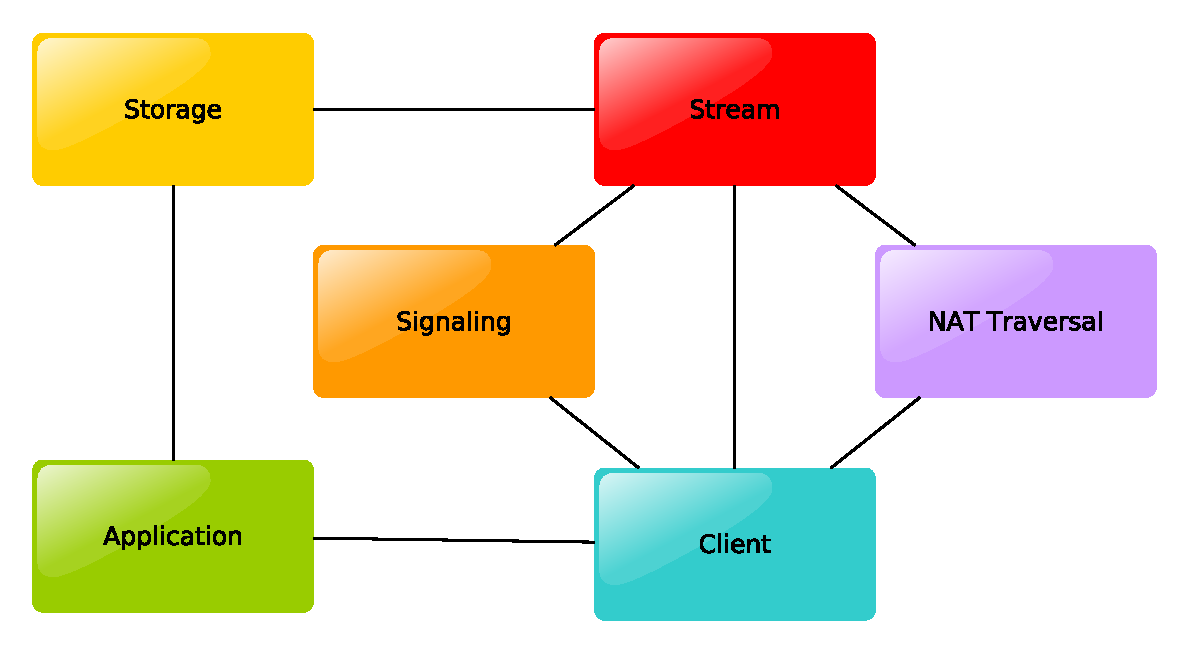
\includegraphics[width=0.8\textwidth]{figures/modules.pdf}
	\caption{System Modules}
    \label{fig:modules}
\end{figure}



\begin{itemize}

\item \textbf{Application module} - responsible for providing information about the relevant modules (\emph{NAT Traversal} and \emph{Signaling}) and user interface to the \emph{Client} in the form of web pages in \ac{HTML} and \emph{JavaScript} libraries through \ac{HTTP}.
 
\item \textbf{Signaling module} - responsible for \emph{Client} and \emph{Stream} coordination which will be performed using \emph{WebSockets}.

 \item \textbf{NAT Traversal module} - \ac{STUN} and \ac{TURN} techniques used by \emph{Client} and \emph{Stream} modules during the \emph{Signaling} phase which ends by establishing the connection between them.

 \item \textbf{Stream module} - responsible to deliver and receive multimedia content from the \emph{Client} using \ac{WebRTC}. 

 \item \textbf{Storage module} - provides two main functionalities: store the model information and media recorded. This is the single module responsible for persistent storage. It stores user and communication data as well as all the data required among user sessions. It is also use to store all the communication streams, so that they can be viewed later.

 \item \textbf{Client module} - responsible for the interaction with the user.

\end{itemize}

%RP Acho que podes escrever muito mais sobre cada componente. Isto está muito curto. Fala de algumas das funções que proporcionam. Vê o que fiz com o Storage Module

%RP também podes fazer um diagrama com vários utilizadores e mostrar quais os streams que vão de e para cada um (mostrar a mistura de som, video, etc).

 
\section{Implementation Proposal}
The infrastructure is composed by: web server, stream server, signaling server, database and video repository.
%RP tens da fazer o paralelo entre isto e os componentes apresentados na secção anterior. O mesmo com a imagem, que parece não estar relacionada. Podes colocar os elementos na mesma posição, ou dentro das caixas da imagem 3.1

\begin{figure}[H]
	\centering
	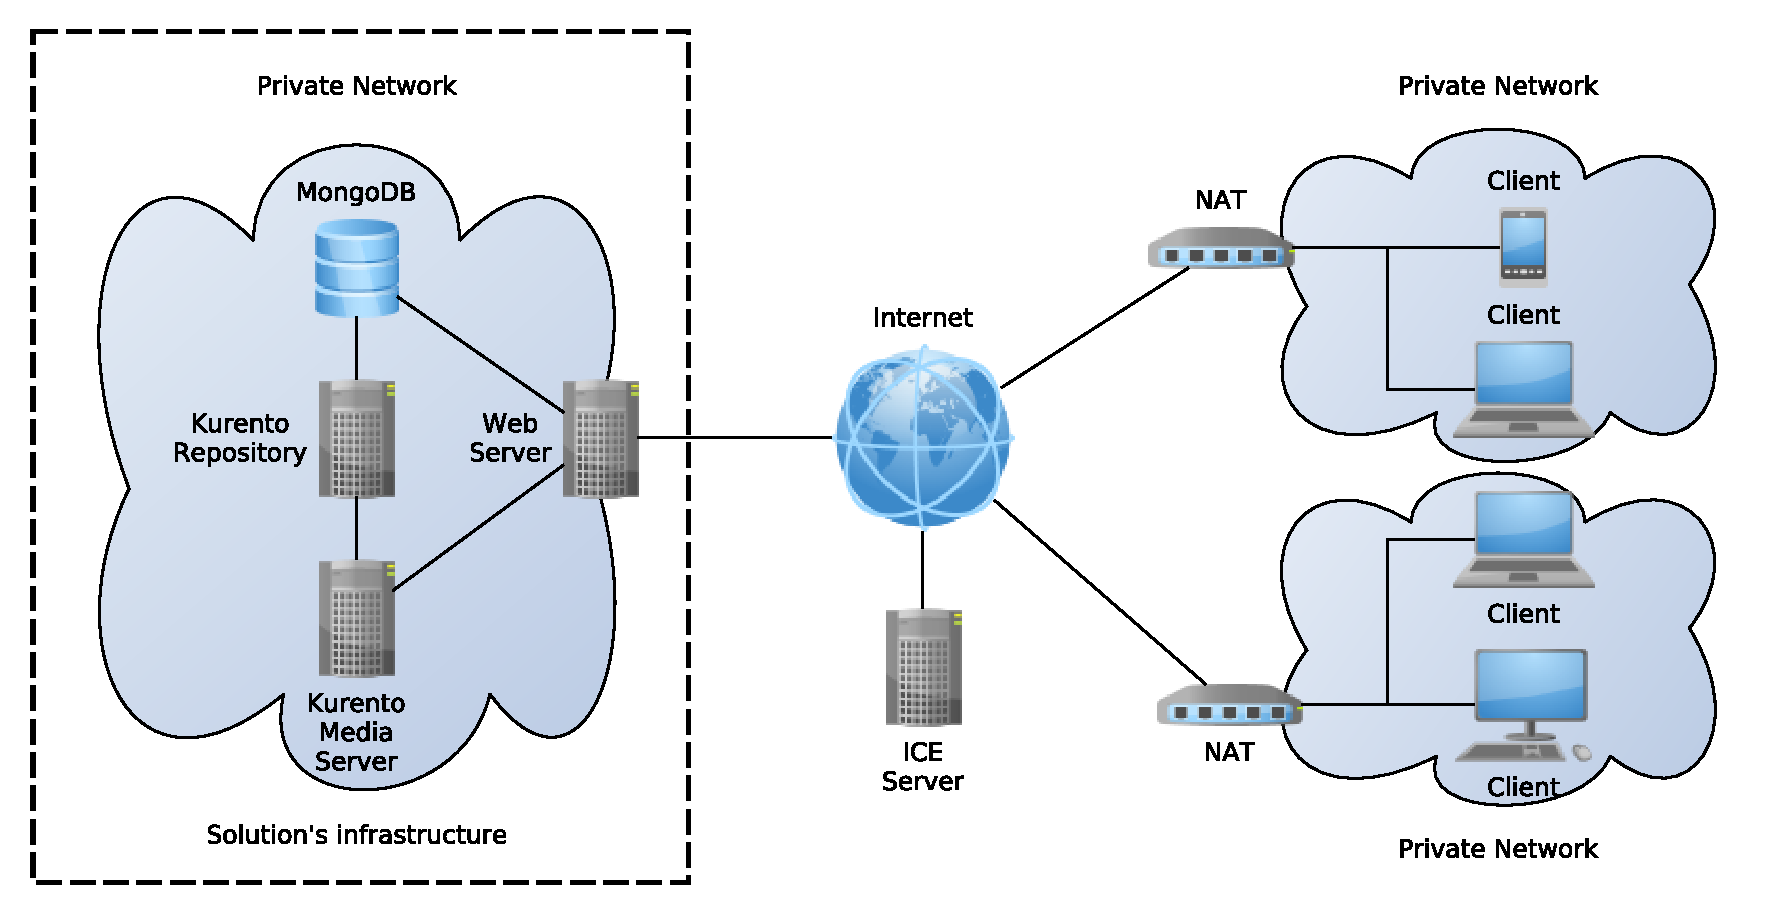
\includegraphics[width=\textwidth]{figures/infrastructure.pdf}
	\caption{System Infrastructure}
\end{figure}

In order to simplify our solution, we propose that the \emph{Application}, \emph{Signaling}, \emph{Stream} and \emph{Storage} modules be implemented within the same server application, so it could be easy to deploy as a single image. To this set of modules, we often call \emph{backend}.

	\subsection{Security and authorization}

Having established that the \emph{backend} modules are placed in the same machine, that helps controlling which resources the client has permission to access as those modules are seen as a private network.
%RP na mesma ``server application'' ou ``machine''? São coisa diferentes! Apresentas vantages de instalar tudo na mesma máquina mas não falas das desvantagens. Menor escalabilidade parece-me ser logo uma delas. Na figura 3.2 aparecem várias máquinas!

To qualify the above we provide public access to \ac{HTTP} server ports, maintaining the access to other components restricted through firewall rules.
%RP qualify?
%RP Imagem com firewall e estes portos? Mas isto já me parece muito detalhe de implementação.
In relation to the database there is no directly access from the outside. All the database information is accessed via our application server which validates the permissions of users on our system.

On the other hand, the access to our streaming servers is also restricted, but clients can connect to them after concluding the signaling phase. This signaling phase may or not proceed in function of the client access permissions. For example, if a user is trying to access a private conference room that he is not a member of nor has an invitation link for, the signaling server refuses to start the signaling phase and the user cannot access the streaming server.

The placement of our streaming servers inside a \ac{NAT} also has an important role with respect to external misuse prevention. Otherwise, placing our streaming servers could allow external clients to perform their own signaling protocol and, as a consequence, use our infrastructure without our consent.

\subsection{Client connections}
	Although the delegation of processing work to clients can improve our system's scalability, we are concerned about using the least resources possible on the client side, as huge resource consumption may drain battery very fast or may even be impossible to run on mobile devices. We are aware that streaming video from clients is already a very intensive task which we cannot avoid but can improve by delegating the most intensive tasks to our servers. 

\begin{figure}
\centering
\begin{minipage}[b]{0.45\linewidth}
	\centering
	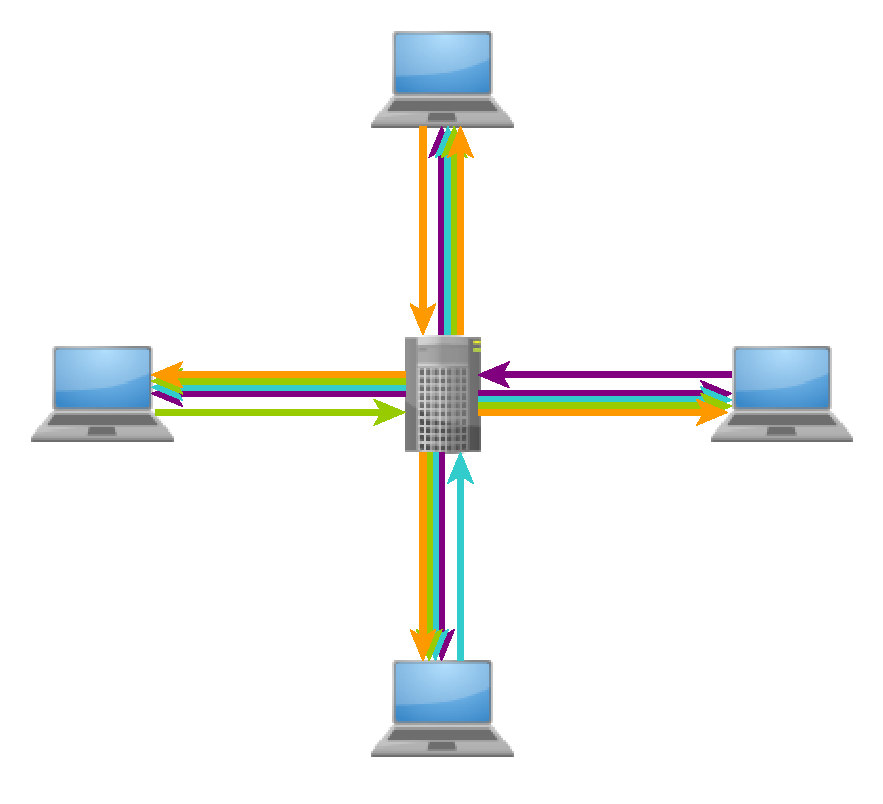
\includegraphics[width=\textwidth]{figures/ccomposite.pdf}
	\caption{Centralized connections}
	\label{fig:central}
\end{minipage}
\quad
\begin{minipage}[b]{0.45\linewidth}
	\centering
	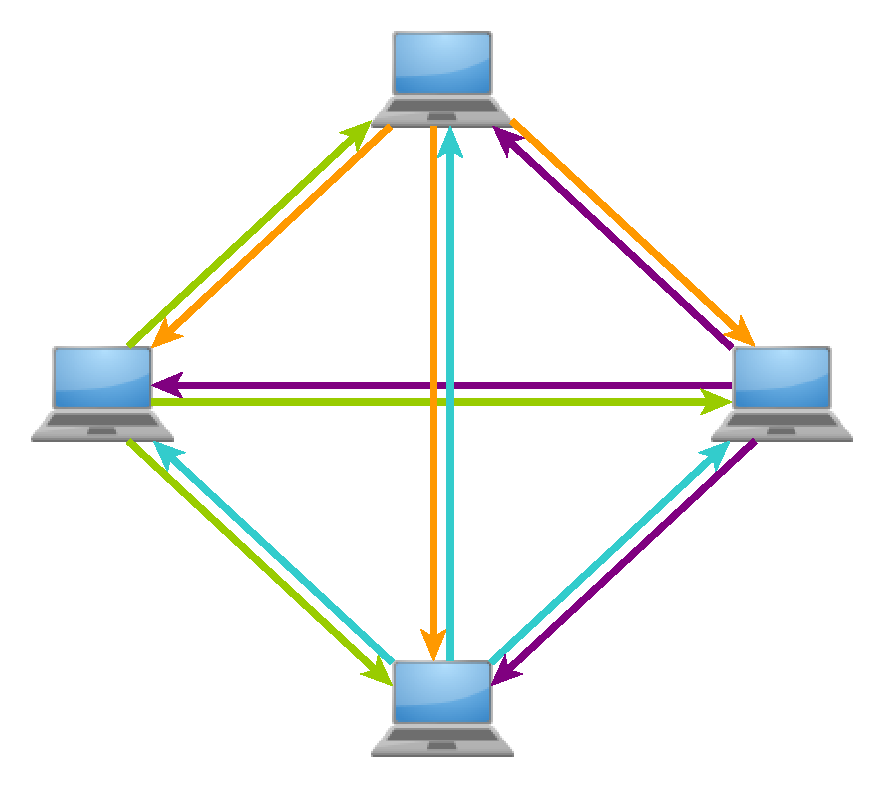
\includegraphics[width=\textwidth]{figures/dcomposite.pdf}
	\caption{Peer-to-Peer connections}
	\label{fig:p2p}
\end{minipage}
\end{figure}

	In this context, each client must only have one \emph{PeerConnection} to our streaming server and content shown to them is changed on demand either being it an individual or a composite view. This approach is centralized, as seen on figure \ref{fig:central}. Otherwise clients could follow a peer-to-peer connection, as seen on figure \ref{fig:p2p}, which would result on maintaining more connections and performing the composition of videos on client side.

	The composition of streams on client side is performed by receiving streams with the best quality possible but, due to undersizing the video of clients into a smaller region, this would result on wasting bandwidth on a quality that is not needed.

	Although the peer-to-peer approach could be used on our system, we conclude that we need to record the video on our streaming server because web clients have a very limited storage and peer disconnections may result on recorded video loss. 

	The same can be concluded to instant message delivery, each client must have only one \emph{WebSocket} connection to the application server which consequently relays the messages to other users.

	Relaying instant messages from clients through the our web servers is easier if all clients are connected to the same server because all messages can be directly delivered without sending messages across multiple web servers. 

	In the context of this thesis, we will not implement sending messages across web servers but, in order to allow our system to scale, we will consider that all conference participants are connected to the same server and our system is scaled by having conference rooms distributed across different servers.

\subsection{Software choices}

Furthermore, we have taken into account the compatibility between the streaming server, database and the operation transformation solutions, in order choose the appropriate framework to implement our web server.
%RP esta secção devia começar aqui, a explicar a escolha das tecnologias/produtos a usar em cada componente. O que tens antes são pormenores que só faz sentido discutir no final. Tens de ir sempre do mais geral para o mais detalhado.

As a result of our study about signaling protocols we have decided to exclude \ac{XMPP} due to the development difficulties that it exposes when using multiple web pages, namely the user re-authentication performed each time a page is loaded and the single tab usage limitation. As a consequence we have not chosen \emph{Jitsi Video Brigde} for stream processing as it uses \ac{XMPP}.

Accordingly, by excluding \emph{Jitsi Video Brigde} we have decided that our solution must use \ac{KMS}. Our web server could be implemented easily with \emph{NodeJS} or \emph{Java} due to the fact \ac{KMS} provides clients for both technologies. But others could also be used as \ac{KMS} also exposes their \ac{API} via \emph{WebSockets}.

Due to the fact we are going to use \ac{KMS} as streaming server solution, we could choose \emph{NodeJS} or any \emph{Java} based web framework for implementing our web application server. One of our criteria for choosing the web framework is the ability to follow the \ac{MVC} paradigm which can help us to organize our code. We have decided to implement our web server with the \emph{PlayFramework}\footnote{\url{https://www.playframework.com/}(acessed March 25, 2016)} using \emph{Java} because of our previous experience with it.

By default, \emph{Kurento Repository} is implemented over \emph{MongoDB}, for convenience our storage model will also use the same database.

Importantly, for the collaborative text editor, we have chosen \emph{OT.js} due to its server and storage implementation choice independence.

For the \emph{NAT Traversal} module, an \ac{ICE} server is not required to be on our infrastructure, as a public \ac{STUN} server can be used for testing our solution. Nevertheless, we recognize that for a production environment we would need to maintain our own \ac{TURN} servers in order to ensure connectivity to all clients.

Not less important, on the client computers, both \emph{Mozilla Firefox} and \emph{Google Chrome} could be installed as web browsers. As such, both should be supported. Libraries such as \emph{jQuery}, \emph{Bootstrap}, \emph{Adapter.js}, \emph{OT.js} can be downloaded from the web server and executed on the client side using any of these two browsers.
%RP relembrar que o IE e o Safari não suportam webrtc?

\begin{table}[H]
\centering
	\caption{Application Architecture}
	\label{table:apparch}
    \begin{tabular}{cccccccc@{}m{0pt}@{}}
	\hline 
\multicolumn{8}{|c|}{\cellcolor{Gray}Application}  &\\[12pt]\cline{1-5}\cline{7-7}
\multicolumn{1}{|c|}{jQuery} & \multicolumn{1}{c|}{HTML5} & \multicolumn{1}{c|}{CSS3 (Bootstrap)} & \multicolumn{1}{c|}{Signaling} & \multicolumn{1}{c|}{~~~~~ot.js~~~~~} & \multicolumn{1}{c|}{\cellcolor{Gray}~~~~~~~~~~~~~~~} & \multicolumn{1}{c|}{adapter.js} &   \multicolumn{1}{c|}{\cellcolor{Gray}~~~~~~~~~~~~~~~} &\\[12pt]\hline
\multicolumn{1}{|c|}{HTTP} & \multicolumn{2}{c|}{User Interface}  & \multicolumn{3}{c|}{WebSocket}    & \multicolumn{2}{c|}{WebRTC}      &\\[12pt]\hline
\end{tabular}
\end{table}

%RP acho interessante o que queres fazer aqui mas acho que está mal conseguido. A linha de baixo, devia ter coisas ao mesmo nível, o que não aconteçe.
% Qual a razão para HTTP estar por baixo do jquery e user interface estar ao lado?
% Sugiro colocar a applicação no meio e as várias interfaces (webrtc, websocket e http) uma de cada lado (esquerda, baixo e direita), indicando o que fica do outro lado (outro cliente, servidor web, servidor stream, etc)

Table~\ref{table:apparch} presents the application architecture and the underlying technologies seen from the user's perspective. \emph{Adapter.js} and \emph{jQuery} will ensure that our application is compatible with the most popular web browsers.
\emph{Bootstrap} will be used to make the user interface more appellative and responsive. With \emph{Bootstrap} it is quite easy to develop applications that adapt to mobile devices with different screen sizes.
%RP bootstrap não aparece na figura!

With respect to displaying content, the synchronization between multimedia elements will be performed through chains of \emph{JavasSript} events or by specifying the interval of time which time content must be visible. Other animations can be implemented with \ac{SVG} embedded on \ac{HTML}.
%RP Caiu do céu! Tens de explicar e ligar melhor a sequencia de texto

\section{Chapter Summary}
\label{architecture:summary}

In this chapter we have shown the modules needed in order to implement our solution.

Several technologies were taken into account for implementing each module, we have studied the pros and cons of each technology and decided the architecture for our solution.



\chapter{Implementation}
\label{chapter:implementation}

%\section{Implementation Options}
%Neste secção devem apresentar as opções de implementação que tinham ao vosso
%dispor, avaliá-las e justificar a escolha que realizaram. Isto pode englobar:
%\begin{itemize}
%    \item Simuladores
%    \item Linguagens e ambientes de programação
%    \item Sistemas operativos
%    \item Hardware
%\end{itemize}
%Fica sempre bem na avaliação colocar uma tabela com as características
%pretendidas e as que são satisfeitas pelas várias opções (tipo catálogo com as
%características dos automóveis). A escolha deve surgir naturalmente, com base na
%opção que tem mais cruzes\ldots

%\section{Architecture}
%Nesta secção devem explicar como implementaram a vossa solução, apresentando
%as simplificações que efectuaram, face ao modelo inicialmente previsto. As
%simplificações devem ser devidamente justificadas. Se for possível, devem indicar
%que estas não põem em causa as contribuições da tese.
%Podem ainda descrever os principais problemas que tiveram e a forma como os
%abordaram e resolveram.

%Se estiverem a usar um simulador devem:

%\begin{itemize}
%    \item explicar o funcionamento do simulador
%    \item explicar as alterações e modelos que desenvolveram no simulador e que permitem validar a vossa ideia
%\end{itemize}

%Se estiveram a desenvolver SW, sem simulador devem:
%\begin{itemize}
%    \item explicar os módulos, interfaces, estruturas de dados, etc\ldots
%\end{itemize}

%Sempre que possível, ilustrem a arquitectura com figuras que demonstrem a
%evolução face à arquitectura da secção anterior. Isto é, usem as figuras anteriores
%e façam as modificações necessárias à obtenção da arquitectura do protótipo.
%\ldots


%RP antes desta secção fala um introdução ao capítulo a explicar o que vai ser apresentado.
%HR done

\section{Data Model}
The data model is a critical component of our solution, as a badly designed model can imply serious difficulties when implementing new features that are not part of the plans. During the course of this project, we had to redesign the model more than once in order to support new features.

%RP devias começar com um overview dos dados que é necessário guardar para a aplicação
%RP ao apresentar o modelo falas de coisas como mensagens para grupos, mas ainda não sabemos nada disso. Na arquitectura, devias falar da concepção, do modelo de comunicação. Que tens utilizadores, grupos, mensagens, chats, convites, etc...
%HR não meti na arquitectura mas adicionei a linha seguinte

In order to offer all the functionalities that we promise, some information about objects must be persistent such as users, groups,relations among users, group memberships, messages, hyper-content, recordings and collaborative editor state.

\subsection {Schema representation}
    \emph{MongoDB} has a slightly different terminology from relational databases. The first big difference is instead of having tables \emph{MongoDB} stores its objects on collections. The analogous data structure to the table row is a document.

    Each \emph{MongoDB} document is represented by a \emph{JSON} object and, as a result, each document may have different attributes within a collection. Needless to say that, by following this approach we do not need to create the collections with a well predefined schema. In fact, we do not need to define it at all but, for reasons of coherence and organization, we represent our database collections as they would have a predefined schema by following the same document structure as we will present in this section.
    %RP a última frase é confusa. O que queres dizer? Reescreve
    %HR está melhor?

    Similarly to relational databases, \emph{MongoDB} requires a primary key (typically of type \emph{ObjectId} and named \emph{"\_id"}) for each document, which is automatically assigned if not specified. 

    In order to define \emph{foreign keys}, we just store them as \emph{ObjectId}s if and only if the foreign keys point to documents within a unique collection, otherwise we need an additional attribute to specify which collection is the \emph{foreign key} pointing at.

    In respect to attributes nullability, \emph{MongoDB} does not enforce a document's attribute to have a not null value, although, for sake of good functionality, we perform those constraints validation programmatically and as such we also represent them in our schema.
    
    An example of schema representation can be seen on Table \ref{table:schema}.

\begin{table}
\centering
\caption{Schema representation}
\label{table:schema}
    \begin{tabular}{|ll|}
        \hline
        \multicolumn{2}{|c|}{\textbf{Collection name}}            \\ \hline
        $\Diamondblack$ \underline{\_id (primary key)} & ObjectId \\ 
        $\medbullet$ Not nullable property name & Property type   \\ 
        $\medcirc$ Nullable property name       & Property type   \\
        $\medcirc$ Reference to document        & ObjectId        \\
        $\medbullet$ Embedded document          & Document        \\ 
        $\medbullet$ Embedded list              & List[Type]      \\ \hline
    \end{tabular}
\end{table}

\subsection {Generic model}

For designing our model we have taken into account generic programming techniques. We observed that operations like searching for an object were quite repeated across different types of objects. 

Our first decision for our model, in order to avoid repeated code, was the isolation of the object's attributes from themselves, so we could apply the search operation to a set of attributes independently of the object type. To this generic set of properties we call data (Table \ref{table:generic}) and each object of this type has a reference to the owner, which is a unique identification number.

\begin{table}
\centering
\caption{Generic data model}
\label{table:generic}
    \begin{tabular}{cc}
        \begin{tabular}{|ll|}
            \hline
            \multicolumn{2}{|c|}{\textbf{Data}}          \\ \hline
            $\Diamondblack$ \underline{\_id} & ObjectId  \\ 
            $\medbullet$ owner          & ObjectId       \\ 
            $\medbullet$ properties    & List[Attribute] \\ 
            $\medcirc$ searchableValues & List[Text]     \\ \hline
        \end{tabular}
        \begin{tabular}{|ll|}
            \hline
            \multicolumn{2}{|c|}{\textbf{Attribute}}     \\ \hline
            $\medbullet$ key            & Text           \\ 
            $\medcirc$ value            & Object         \\ 
            $\medbullet$ identifiable   & Boolean        \\ 
            $\medcirc$ readPermissions  & List[ObjectId] \\ 
            $\medcirc$ writePermissions & List[ObjectId] \\ \hline
        \end{tabular}    
    \end{tabular}
\end{table}

The owner's identification number by itself is not sufficient to identify an object, as objects from different types can have the same identification number. In order to solve this problem, when an object is created, its correspondent data must contain the owner's object type. 
%RP mas o _id é apresentado com sendo uma chave primária na figura 4.2, logo única!
%HR "The owner's identification number" corriji, não me referia ao "_id"

Whenever an attribute is created, its name, value and indentifiability must be specified. The set of objects that can read and write that attribute must also be defined. 
In regard to our permission mechanism, if the read or write sets are not specified we assume the attribute is readable and writable by everyone. Conversely if the read and write sets are empty, nobody is allowed to read or write the attribute. Implicitly, if an entity can write an attribute, it can also read it.

In particular, if all attributes were searchable, it could be simple to search for attributes that could reveal sensible information about an object. For example if we consider that a user could have a health related attribute, searching by a disease would reveal which users could suffer from a certain disease. The leak of that kind of information could, for instance, change the agreement between users and health insurance companies. For this reason only the specified attributes as searchable will be taken into account when performing keyword searches.
%RP era melhor que o exemplo fosse relativo à tua aplicação e não algo abstracto como saúde.
%RP Dás permissões de leitura e escrita a objectos. Normalmente é a utilizadores. Explicar relação. Assumo que sejam aqui referenciados apenas objectos que representam utilizadores

Another important attribute specification is the owner identifiability, which tells us if the attribute identifies the object. This specification lets us create abstract authentication services. For example a user can login into our system by providing any attribute that identifies himself, \emph{e.g.} the e-mail, but others are possible like the user name or cellphone number. 

Not less important, in order to get an object's properties efficiently, we have created an index over the \emph{owner} attribute. We have also created an index over the \emph{searchableValues} in order to improve the keyword search performance.

In summary, with this model we can perform search and identification of any kind of objects, as we will see on the following models. In particular, the \emph{user} and \emph{group} models are using this generic model for storing their attributes. 
% Not less important, attributes can specify aggregations of objects. For example, the user role is an aggregator property that within users it allows the identifaction of each one is administrator. This aggregation specification is independent from the object type, so it is possible to search for the administrative role and return users and groups of users that contains that property. <= [currently this operation is possible but it is not specified]


%RP antes de falares de cada modelo, que tal incluir uma figura com a relação entre os vários tipos de dados. Mesmo não sendo SQL, as relações existem conceptualmente e falas em chaves estrangeiras, pelo que tal figura faz sentido e ajuda a perceber.

\subsection{User model}

The user model is not tied to the user attributes (Table \ref{table:user}), the information maintained in this model is just used for authentication purposes. Passwords are not stored in plain text, instead we apply hashing and salting techniques \cite{password} in order to make it harder to decode the password by an attacker. Accordingly, we use \emph{SHA-1} and a random salt per user with 32 characters.
%RP Table x, Figure y, etc é sempre maiusculas.

\begin{table}
\centering
\caption{User model}
\label{table:user}
    \begin{tabular}{|ll|}
        \hline
        \multicolumn{2}{|c|}{\textbf{User}}         \\ \hline
        $\Diamondblack$ \underline{\_id}  & ObjectId  \\ 
        $\medbullet$ hash           & Text          \\ 
        $\medbullet$ salt      & Text               \\ \hline
    \end{tabular}
\end{table}

\subsection{Relation model}
% HR-FINAL - Sim isso, relações em geral, user-grupo, user-user, grupo-grupo, user-carro, user-escola... no fundo entidades, como está escrito

A relation between two entities $e_1$ and $e_2$ is represented by the pair $e_1\rightarrow e_2$ (Table \ref{table:relation}), where $e_1$ is the source and $e_2$ is the target. This relation is said to be bi-directional if and only if it also exists the relation $e_2\rightarrow e_1$.

\begin{table}
\centering
\caption{Relation model}
\label{table:relation}
    \begin{tabular}{|ll|}
        \hline
        \multicolumn{2}{|c|}{\textbf{Relation}}     \\ \hline
        $\Diamondblack$ \underline{\_id}  & ObjectId  \\ 
        $\medbullet$ source           & ObjectId    \\ 
        $\medbullet$ target      & ObjectId         \\ \hline
    \end{tabular}
\end{table}

A user can only interact with friends or with group members. In order to validate a friendship, both users must agree on that friendship, in other words it, there must exist a bi-directional relation between both users.

In order to improve the performance of queries over the \emph{Relation} collection we have created indexes on the \emph{source}, \emph{target} and also on the pair composed by both attributes.

\subsection{Group model}

A conference room, which is the environment where users communicate among themselves, is represented persistently by a group of participating entities (in general users but our system allow other types of entities). A conference room is composed by only online users and does not need to be stored on database.

A group is composed by an \emph{id}, \emph{inviteToken} and a \emph{visibility} as shown on Table \ref{table:group}.
Moreover, a group can be public or private. If the group is public, then it is visible to all users that maintain a friendship with a member of this group. If the group is private, then it is only visible to its members.


\begin{table}
\centering
\caption{Group model}
\label{table:group}
    \begin{tabular}{cc}
        \begin{tabular}{|ll|}
            \hline
            \multicolumn{2}{|c|}{\textbf{Group}}        \\ \hline
            $\Diamondblack$ \underline{\_id}  & ObjectId  \\ 
            $\medcirc$ inviteToken           & Text     \\ 
            $\medbullet$ visibility      & Text         \\ \hline
        \end{tabular}

        \begin{tabular}{|ll|}
            \hline
            \multicolumn{2}{|c|}{\textbf{GroupMembership}}  \\ \hline
            $\Diamondblack$ \underline{\_id}  & ObjectId      \\ 
            $\medbullet$ groupId            & ObjectId      \\ 
            $\medbullet$ userId & ObjectId                  \\ \hline
        \end{tabular}    
    \end{tabular}
\end{table}


The group membership is a special case of relation, where the target entity is always a group.
When a group is created, a group membership is automatically assigned to its creator.

Entities that have a membership with a group can create more memberships by sharing an invite token or by specifying new group members. This invite token is used to create an invite \ac{URL} that if shared with other users allow them to join the group. Invite tokens can be deleted or regenerated with a different value.
%RP isto quer dizer que quem tem o token se pode juntar ao grupo? Explicar. O que impede alguém de o partihar com outros?
%HR done

In order to improve performance of queries over \emph{GroupMembership} collection we have created indexes on the \emph{groupId}, \emph{userId} and also on the pair composed by both attributes.


\subsection{Message model}

A message is composed by its content, time of creation and source and target identification numbers (Table \ref{table:message}). The message's target could reference any object, but our application is only handling messages to groups.

\begin{table}
\centering
\caption{Message model}
\label{table:message}
    \begin{tabular}{|ll|}
        \hline
        \multicolumn{2}{|c|}{\textbf{Message}}      \\ \hline
        $\Diamondblack$ \underline{\_id}  & ObjectId  \\ 
        $\medbullet$ source           & ObjectId    \\ 
        $\medbullet$ target      & ObjectId         \\ 
        $\medbullet$ content      & Text            \\ \hline
    \end{tabular}
\end{table}

In order to query for recent messages for a given target, we use the oldest message's \emph{\_id}, which is sequential, in order to find messages with a newer \emph{\_id}.

In order to improve performance of queries over \emph{Relation} collection we have created indexes on the \emph{target} attribute and also on the pair composed by \emph{target} and \emph{\_id} attributes for finding and sorting the messages received by an entity more efficiently. 

%RP pela justificação não consigo perceber para que serve a chave no par target e _id
%HR in order to find recent messages (não tinha explicado)

\subsection{Hyper content model}

During a group conversation, it is possible to create time annotations for making it easy to access that time either for searching or sharing with other users.
A time annotation (Table \ref{table:hyper}) contains a title, the correspondent group identification number and the time itself.

The hyper content is used to synchronize content among users during a conversation. Table \ref{table:hyper} shows that every hyper content must have a start and ending time, the correspondent group identification number and the content itself, in the form of text. Beside those attributes, in order to perform queries over the \ac{HTML} contents with more precision, we have added an additional \emph{searchableContent} attribute. It contains just the searchable content extracted from the content, by excluding the \ac{HTML} tags and parameters using \emph{Jsoup}\footnote{\url{http://jsoup.org/} (Accessed April 11, 2016)}.

In the point o view of a user, a time annotation is just a simple way to associate a time stamp to a topic in order to make it easier to find. On the other hand, the hyper-content is more complete than time annotations, except they are not visible on the timeline. In addition to time annotations, hyper-contents have a duration and content that can be superimposed to video.

%RP explica melhor a diferença entre HyperContent e Time Annotation do ponto de vista do utilizador / funcionalidade proporcionada.
%HR done

\begin{table}
\centering
\caption{Hyper content model}
\label{table:hyper}
    \begin{tabular}{cc}
        \begin{tabular}{|ll|}
            \hline
            \multicolumn{2}{|c|}{\textbf{HyperContent}}  \\ \hline
            $\Diamondblack$ \underline{\_id}  & ObjectId \\ 
            $\medbullet$ groupId            & ObjectId   \\ 
            $\medbullet$ start              & Date       \\ 
            $\medbullet$ end                & Date       \\ 
            $\medbullet$ content            & Text       \\ 
            $\medbullet$ searchableContent  & Text       \\ \hline
        \end{tabular}

        \begin{tabular}{|ll|}
            \hline
            \multicolumn{2}{|c|}{\textbf{TimeAnnotation}}  \\ \hline
            $\Diamondblack$ \underline{\_id}  & ObjectId   \\ 
            $\medbullet$ groupId            & ObjectId     \\ 
            $\medbullet$ title & Text                      \\ 
            $\medbullet$ time & Date                       \\ \hline

        \end{tabular}    
    \end{tabular}
\end{table}

For example the content showed in Listing \ref{lst:jsoup} would produce the searchable content "Click here!".

\begin{minipage}{\linewidth}
\begin{lstlisting}[caption={Example of HTML content},label={lst:jsoup},language=JavaScript]
<div class="subtitle">
    <a href="/">Click here!</a>
</div>
\end{lstlisting}
\end{minipage}

In order to improve the performance of searching content and calculate interval intersections, we have created indexes over the following sequences of attributes: 

\begin{itemize}
\item{\emph{\{groupId,start,end\}} $\rightarrow$ for finding visible contents for a given time  within a group (intersections).}
\item{\emph{\{groupId,start\}} $\rightarrow$  for finding contents that starts after a given time within a group (for pre-loading).}
\item{\emph{\{groupId,searchableContent\}} $\rightarrow$ for searching contents by keywords within a group.}  
\end{itemize}

\subsection{Collaborative Content model}

Within a conversation, users can write documents collaboratively. As we can see in Table \ref{table:collaborative}, each document has a content and a reference to the correspondent group. 


\begin{table}
\centering
    \caption{Collaborative content model}
    \label{table:collaborative}
    \begin{tabular}{|ll|}
        \hline
        \multicolumn{2}{|c|}{\textbf{CollaborativeContent}} \\ \hline
        $\Diamondblack$ \underline{\_id}  & ObjectId        \\ 
        $\medbullet$ groupId            & ObjectId          \\ 
        $\medcirc$ content            & Text                \\ \hline
    \end{tabular}
\end{table}

In order to improve the performance of finding the group's content we have created and index over the \emph{groupId} attribute.

\subsection{Recording model}

During a conversation, users may allow sharing their web cameras. By doing so, their video is stored in recording chunks. Each chunk, described in Table \ref{table:recording}, represents an interval of time $T=\big[c^{start},c^{end}\big[$ of the video stream. It also contains the media's \ac{URL}, a reference to a group, an owner identification number and the correspondent \emph{WebSocket} session id.
    
    The media's \ac{URL} is the location where \emph{Kurento Repository} stores one chunk of video (including audio) which is used to playback on users demand.

    %RP ainda não tenho forma de perceber o que é o websocket session id. Nunca falaste de websockets antes, quanto mais disto! Nem do media URL, é gravado ou webrtc (dispositivo do utilizador)?
    
    In order to allow the same user to have different devices, storing just the \ac{URL} with an associated user id is not enough. In this case, one more parameter is needed to differentiate the different \emph{webSocket} sessions opened by the same user. For this reason we had to associate a random session identification number to each \emph{webSocket}.

\begin{table}
\centering
    \caption{Recording model}
    \label{table:recording}
    \begin{tabular}{cc}
        \begin{tabular}{|ll|}
            \hline
            \multicolumn{2}{|c|}{\textbf{RecordingInterval}}  \\ \hline
            $\Diamondblack$ \underline{\_id}  & ObjectId      \\ 
            $\medbullet$ groupId            & ObjectId        \\ 
             $\medbullet$ start             & Date            \\ 
            $\medbullet$ end                & Date            \\ \hline
        \end{tabular}   
        \begin{tabular}{|ll|}
            \hline
            \multicolumn{2}{|c|}{\textbf{RecordingChunk}}  \\ \hline
            $\Diamondblack$ \underline{\_id}  & ObjectId     \\ 
            $\medbullet$ groupId            & ObjectId     \\ 
            $\medbullet$ owner           & ObjectId        \\ 
            $\medbullet$ sessionId          & Text         \\
            $\medbullet$ start              & Date         \\ 
            $\medbullet$ end                & Date         \\ 
            $\medbullet$ url               & Text          \\ \hline
        \end{tabular}
    \end{tabular}
\end{table}



A set of chunks $S=[c_1,c_2,\ldots,c_n]$ is said continuous if $\forall c_i\in S, \exists c_j \in S$ where $j\neq i$ and $c_i^{start} = c_j^{end} \vee c_i^{end} = c_j^{start}$. 
A recording interval represents a continuous set of recording chunks.

In respect to find which chunks to play given a specified time (which is the current time in a user's perspective), we must select the chunk with an ending instant immediately after the current time, if the chunk's beginning is placed before the current time we have to play it instantaneously otherwise the chunk's beginning will occur after the current time and therefore we have to schedule the playback.

On the other hand, we use the fact that \emph{\_id}'s are sequential in order to determine adjacent chunks, for example, if we need to find the next chunk to play, we have to sort all elements by \emph{\_id} (which on \emph{MlongoDB} is already sorted by default) and select a chunk with an \emph{\_id} immediately after the current one. 

In order to improve the performance of searching recording chunks and calculate which chunks are going to be reproduced, we have created indexes over the following sequences of attributes: 
\begin{itemize}
    \item{\emph{\{groupId,start,end\}} $\rightarrow$ for finding all available chunks for a given time} 
    \item{\emph{\{groupId,sessionId,end\}} $\rightarrow$ for finding chunks that ends after a given time within a session}
    \item{\emph{\{groupId,owner,end\}} $\rightarrow$ for finding chunks that ends after a given time within a user (for a different session) or group}
    \item{\emph{\{groupId,sessionId,\_id\}} $\rightarrow$ for finding chunks that follow a given \emph{id} within a session}
    \item{\emph{\{groupId,owner,\_id\}} $\rightarrow$ for finding chunks that follow a given \emph{id} within a user or group}
\end{itemize}
%RP os _id não são únicos? Para que servem os index que os incluem?
%HR done, for finding adjacent chunks

%RP para a intercepção não precisaste de usar o start, apenas o end?
%HR exactly, if there is no intersection taking into account the "end" at least I can schedulle the next player (after the end)


Not less important, we have also created an index over the \emph{RecordingInterval}'s \emph{groupId} attribute for listing all intervals within a conference room. 
%RP olha outra coisa nova! Ainda não falaste de conference rooms!
%HR "conference room" dá-se no contexto de um "group", era para não estar sempre a repetir. Qualquer das formas adicionei esse pormenor na seccao do grupo.



\section{Signaling Protocol}

As we have already mentioned on our related work, \ac{WebRTC} does not implement the signaling protocol, which is used to establish connections between peers. This connection may be direct using \ac{STUN} or relayed by a \ac{TURN} server in case of direct communications are not possible.

The signaling protocol plays a fundamental role on our solution. Taking into account the choices we have based on our related work, we have decided to implement our own signaling protocol in order to use \ac{WebRTC} on our solution.

Although we have mentioned that the signaling protocol is used to establish connections between peers, on our system our media server (\ac{KMS}) is a peer that receives video streams and sends to its connected clients. 

In a general view, the signaling protocol is used to share connection and media properties between two peers. In order to ease the understanding of our signaling protocol, we have created a sequence diagram that is represented on Figure \ref{fig:signaling2}\footnote{Although two \ac{ICE} servers are shown they are, in fact, the same. Showing just one \ac{ICE} server would be difficult to draw.}.
%RP devias começar com uma introdução a explicar que tiveste de desenvolver um protocolo para coordenar a interacção dos clientes com o servidor e entre clientes (?).
%RP explicar quando é usado (começar chamada, terminar, juntar, chat(?), edição colaborativa (?), etc).
%HR done


\begin{figure}
    \centering
    \begin{subfigure}{}
    	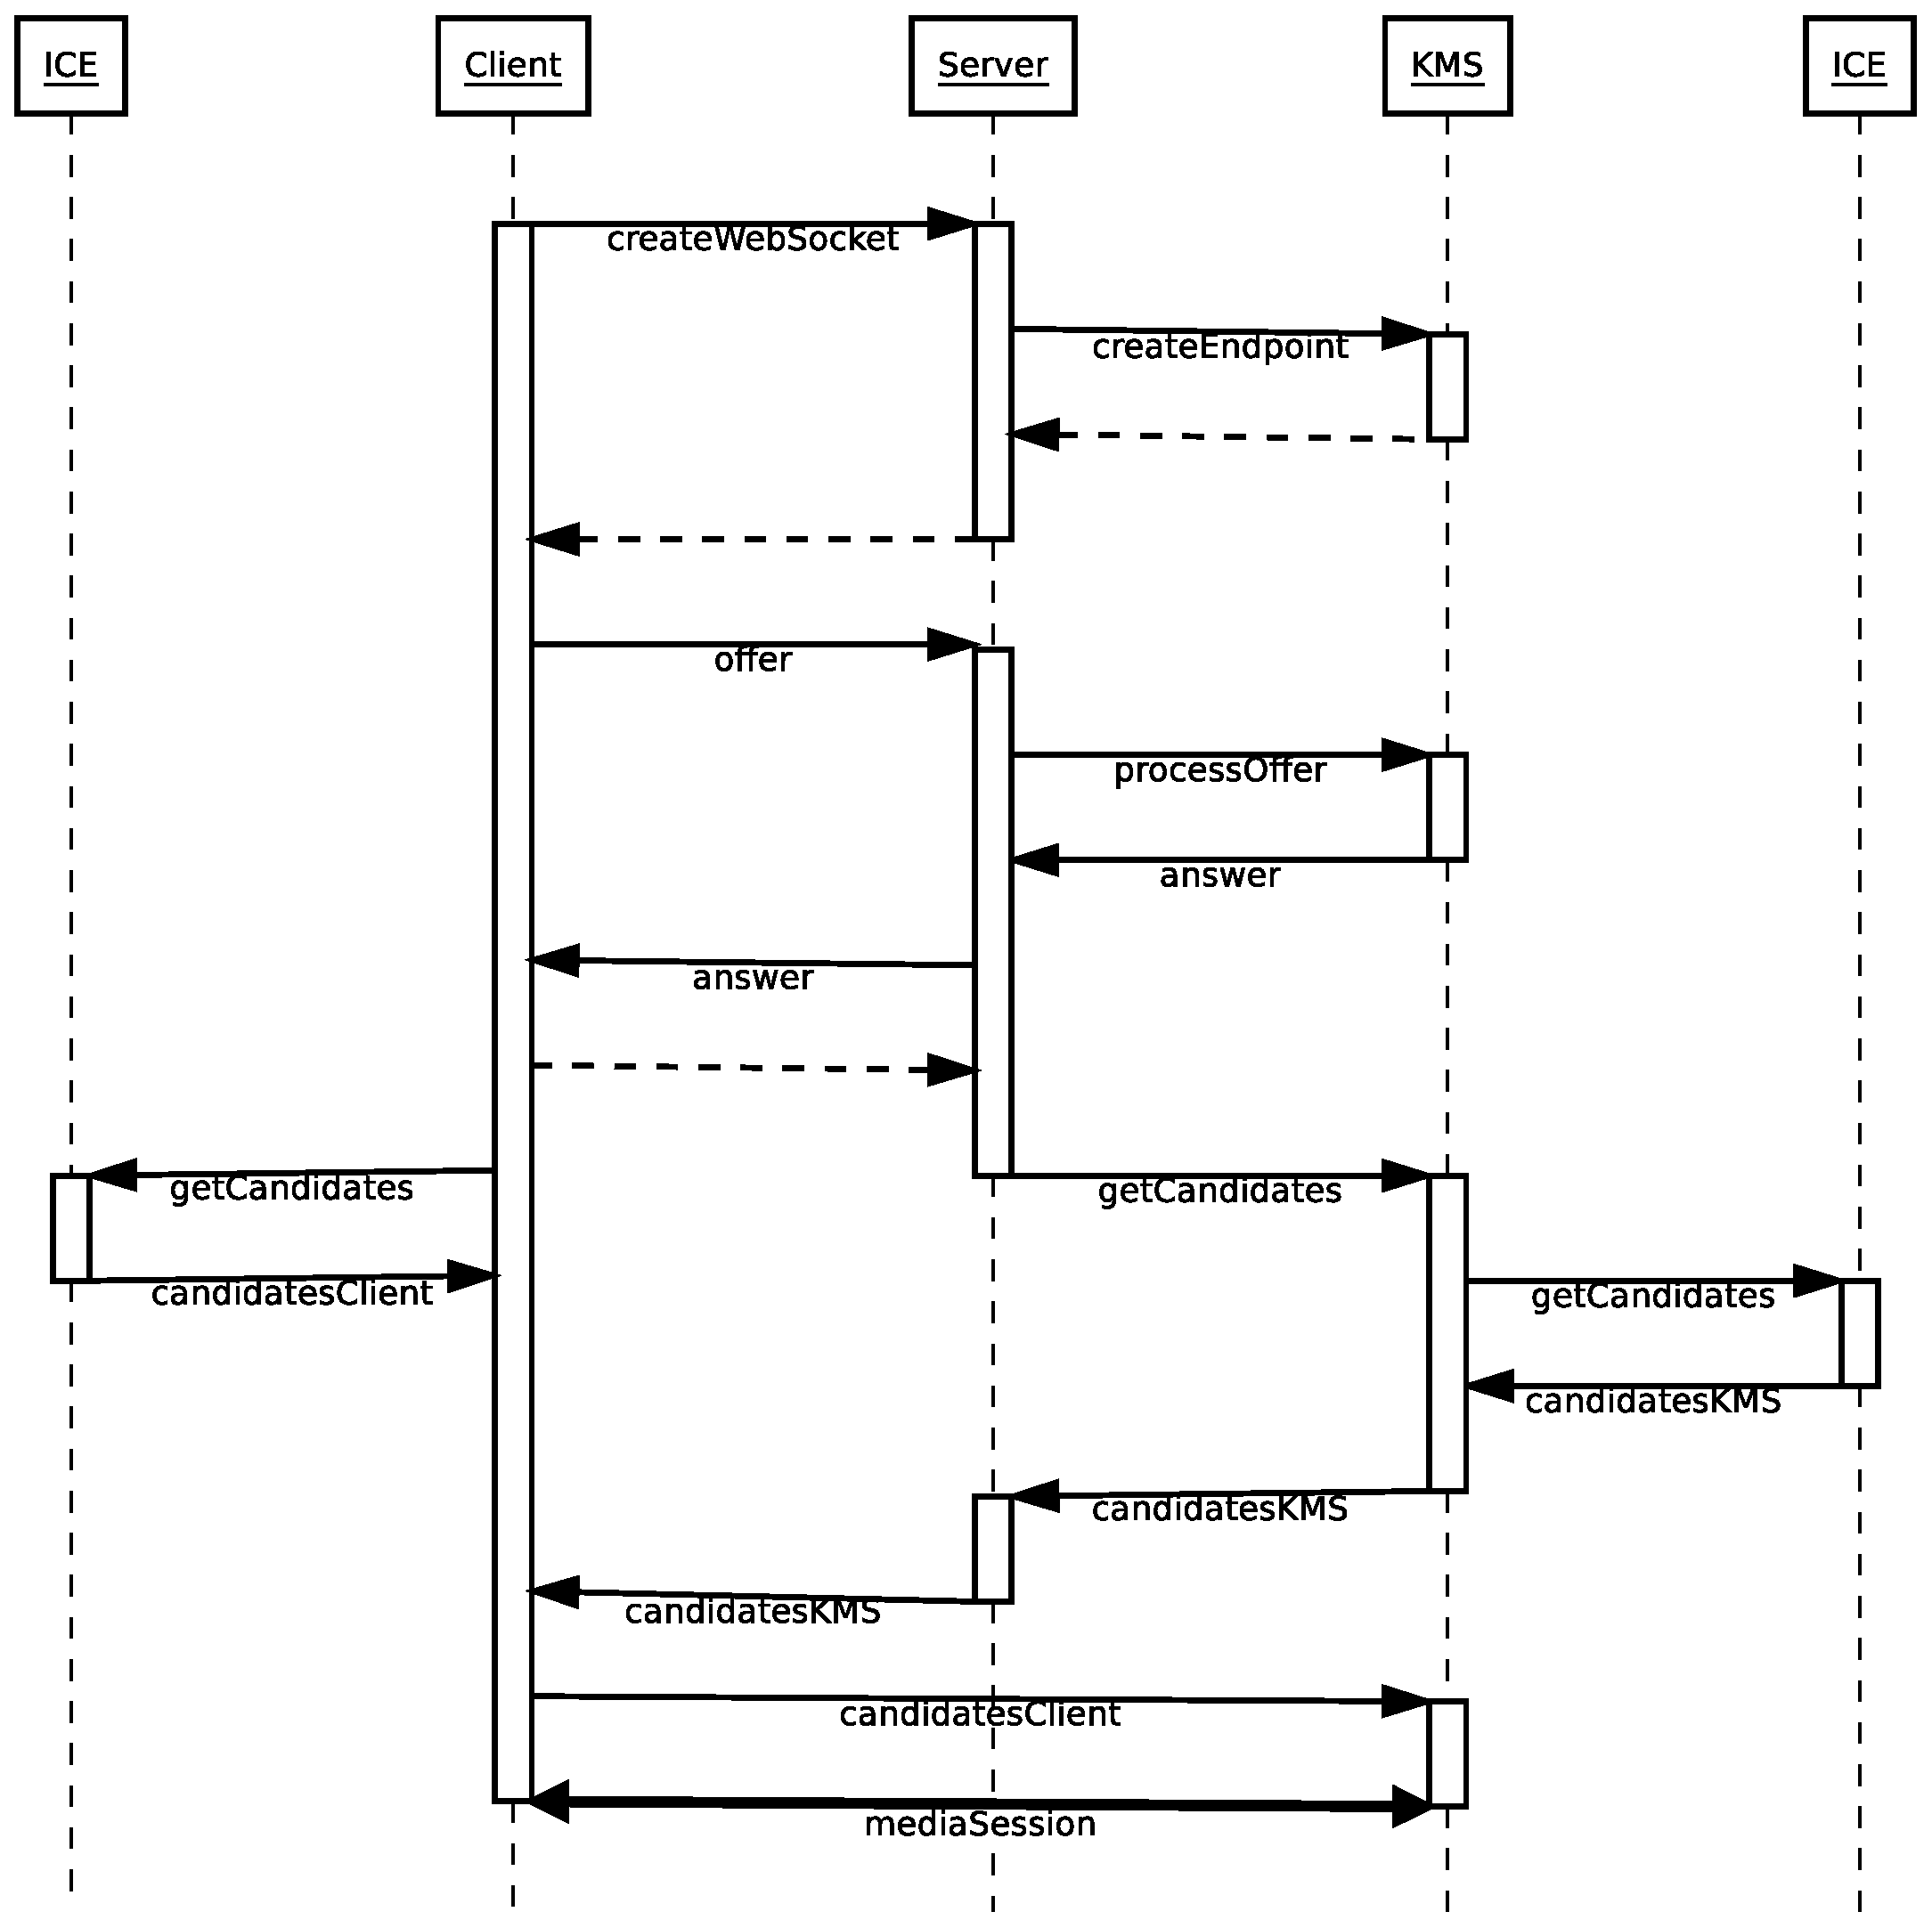
\includegraphics[width=0.9\textwidth]{figures/signaling}
    \end{subfigure}
    \caption{Signaling sequence diagram}
    \label{fig:signaling2}
\end{figure} 


Before the signaling protocol starts, the user must be authenticated. After the user provide the correct credentials, it receives an \ac{HTTP} \emph{cookie} from our server in order to be identified in the following \ac{HTTP} requests.

%RP faz sentido haver dois ICE? Se queres colocar 2 dá-lhes nomes diferentes (nem que seja cliente e servidor ou 1 e 2).

After the web application server validates the user access, the signaling protocol allows the users to directly connect to the \ac{KMS}, which is placed in a private network, and lets the application server and users negotiate media types and encoding information to use during the conversation.
%RP o it em ``it allows'' é quem? webserver ou signaling protocol?
%HR done
We considered implementing the signaling protocol using \ac{HTTP} messages.
However, they would transport extra information such as \ac{HTTP} headers and would follow a request-response signaling mechanism which would not be the best option, as multiple ICE candidates can arrive at any time. Using a \ac{REST} \ac{API} over \ac{HTTP} for signaling and allowing other methods to be called at the same time would lead to opening multiple \ac{TCP} connections at the same time.

Instead, if we create a \emph{WebSocket} \ac{API}, we only need one \ac{TCP} connection and, at the same, provide bi-directional communications without additional headers. Moreover, using \emph{WebSocket} allows the application server to send messages asynchronously to the client without the client having to request it, which can be slightly faster than using \ac{HTTP} which is based on a request followed by a response.
%RP em vez de slighhtly faster não queres antes enfatizar que pode ser antes o servidor a iniciar a comunicação, de forma assincrona?
%HR done
Our signaling protocol consists of sending and receiving \ac{JSON} formated messages, \emph{e.g.} Listing \ref{lst:msgtype}, over WebSockets by both the application server and the client. 

\begin{minipage}{\linewidth}
\begin{lstlisting}[caption={General structure of our WebSocket messages},label={lst:msgtype},language=json]
{
	"cmd":<cmd>,
	"data":<data>
}
\end{lstlisting}
\end{minipage}

When a user enters a group conference, after the page is completely loaded, a WebSocket is created to maintain a connection with our web servers. 
But before creating the web socket, we must identify the user and check if he has permissions to participate in the conference. The user identification is done by retrieving the session id from the cookie provided by the user-agent (web browser) through the \ac{HTTP} headers.
%RP não é bem o user que fornece o cookie. é o user-agent (browser). Convém ser preciso.
%HR done
The web application server retrieves all the information needed from the database in order to check if the user has permissions to join that conference room. It is important to save the user identification before the \emph{WebSocket} connection is created because, after the handshake is performed by the \emph{WebSocket} protocol\cite{rfc6455}, the \ac{HTTP} context is lost.
%RP socket -> websocket?

When the connection is established between the application server and the client, a \emph{PeerConnection} is created on the client and immediately after, an \ac{WebRTC} endpoint is created on the server, specifying a possible set of \ac{ICE} servers to connect.
%RP Usa Application server e não apenas server. Há muitos servers.

At this stage, the web application's user is asked if he wants to share its camera and microphone, share screen or just receive streams from the server. If the user decides to perform a screen share, \emph{adapter.js}\footnote{\url{https://github.com/Temasys/AdapterJS}(accessed March 15, 2016).} may ask to install a plug-in if the browser does not support screen sharing \footnote{\url{http://iswebrtcreadyyet.com/} (Accessed May 11, 2016)}.
%RP web app user? OU apenas client user?
%RP foot note com exemplos de browsers que aceitem screen sharing?
%HR done
If the user decides to share either from camera or screen, \emph{getUserMedia} is called with the correspondent constraints in order to obtain a local stream. We use the constraints presented on Listing \ref{lst:constraints}. 

\begin{minipage}{\linewidth}
\begin{lstlisting}[caption={Media constraints},label={lst:constraints},language=JavaScript]
var screenShareConstraints = {	
	"video": {
		"mediaSource": "window" || "screen"
	}, 
	"audio": false
};
var cameraMicrophoneConstraints = {
	"audio":true, 
	"video":true 
};
var receiveOnlyConstraints = {
	"offerToReceiveAudio":true,
	"offerToReceiveVideo":true
};
\end{lstlisting}
\end{minipage}

If the user decides to share his camera or screen, a pop-up is raised in order to ask the user to give permission to share those resources. If the resources are shared successfully, the user agent creates an offer like Listing \ref{lst:sig01}, sets a \emph{local session description} to its \emph{PeerConnection} and sends it through the WebSocket to the Application Server.
%RP usas ``user'' duas vezes, uma para te referires ao utilizador e outra ao browser (user agent).
If the resources are not shared or the user specified to receive stream only, an \ac{SDP} offer is created specifying the constraints for receiving only video and audio.
%RP offer -> SDP offer?

\begin{minipage}{\linewidth}
\begin{lstlisting}[caption={Offer created by client},label={lst:sig01},language=json]
{
	"cmd":"offer",
	"data":{
		"type":"offer",
		"sdp":<sdp>	// omitted for brevity
	}
}
\end{lstlisting}
\end{minipage}

The \emph{local session description} contains the session identifier, codecs, containers, transport protocols and ports used per media type. The \emph{local session description} is useful to conclude if the client is receiving only, which means that \ac{KMS} does not need to mix, record nor analyze streams coming from the user's \ac{WebRTC} endpoint. 

The server receives and processes the offer and sets the \emph{remote session description} to its client associated \ac{WebRTC} endpoint. Then a \emph{local session description}, like the one presented in Listing \ref{lst:sig02}, is created on the server and sent back to the client. After that, the server tries to gather \ac{ICE} candidates.
%RP listing -> Listing

\begin{minipage}{\linewidth}
\begin{lstlisting}[caption={Answer created by KMS},label={lst:sig02},language=json]
{
	"cmd":"answer",
	"data":{
		"type":"answer",
		"sdp":<sdp>	// omitted for brevity
	}
}
\end{lstlisting}
\end{minipage}

The client receives the server answer, sets the \emph{remote session description} and gets the ice candidates from the \ac{ICE} server.
%RP tens ``ice'', ``\ac{ICE}''. Acho que também já vi ``ICE''. Convém ser sempre igual!

Subsequently, after a while both the server and client receive the \ac{ICE} candidates that allow the client to connect directly to \ac{KMS} and vice-versa. The candidates are received at the client which sets them to its \emph{PeerConnection}. The same is done on the server which receives the \ac{ICE} candidates like on Listing \ref{lst:sig03} from the client and propagates them to \ac{KMS}.
%RP A figura 4.1 precisa de vir antes deste texto todo, para ser mais fácil de perceber.
%RP também tens de explicar porque razão escolheste colocar o KMS numa rede privada. Se está numa rede privada, usas NAT ou um proxy (socket) para estabelecer a ligação?
%HR uso NAT, falei disso na arquitectura, serve para o cliente não aceder directamente ao servidor de streaming e realizar o seu proprio protocolo de sinalizacao (uso indevido por parte de atacantes)

\begin{minipage}{\linewidth}
\begin{lstlisting}[caption={ICE candidates sent by KMS and client},label={lst:sig03},language=json]
{
	"cmd":"iceCandidate",
	"data":{
		"sdpMLineIndex":0,
		"candidate":"candidate:15 1 TCP 843056127 146.193.224.20 48828 typ srflx raddr 192.168.1.105 rport 48828 tcptype passive",
		"sdpMid":"audio"
	},
}
\end{lstlisting}
\end{minipage}

An \ac{ICE} candidate contains an \ac{IP}, port, used transport protocol and an attribute named \emph{sdpMLineIndex} that is used for mapping to the \emph{remote session description} media type.
In addition, both intervenients test the connectivity of each \ac{ICE} candidate. When a connection is established, the user and server start to interchange stream data but other \ac{ICE} candidates may arrive with better connections. When that happens, the connection changes seamlessly. 

Having the media session established, the server starts to record any received stream and the client creates an \ac{URL} correspondent to the stream location.


%RP não falas nada sobre chats, etc! Não há signalling para isso?
%HR não, só video e audio, chat é websockets
\section{Stream Recording}
	In this section we describe our approaches for the stream recording implementation, namely recording on the client side and server side.

\subsection{Client side recording}
	In order to record used shared streams, our first approach consisted on recording video and audio streams into blobs of limited duration. Because each user was recording directly from their shared local resources, we achieved the best stream quality.

	After recording, each block was uploaded to our server through \ac{HTTP} and saved into the file system, the block meta-data was created and inserted on our database. Each block meta-data contained the file's location for the recorded block, the starting date, duration, user identification and group identification. When the file was completely saved the meta-data was advertised to the remaining users. This meta-data was simply used to refresh the user interface, the meta-data was completely discard after that because an huge amount of small blocks meta-data would use more and more memory as time went by. 

	The process to play a video was quite simple, the user specified which user and date was intended to play, the server calculated the intersection between the requested date and the block bounds and returned the file to the client.

	Although this idea was fairly simple, we couldn't achieve seamless sequential block switching. Downloading the video file always toke a noticeable amount of time. To solve this problem while we were playing a block, the next one was downloading in parallel so when the current block finished playing we would have an available block to play. 

	Block switching became more acceptable, but switching the \ac{URL} always produced a flash. We solved this problem by having two layers and set the \ac{URL} to the back layer, the front layer frozen with the last frame, then we changed the back layer to front. 

	After we implemented our recording solution using this approach, we tested locally and remotely. For remote connections we observed a fairly high bandwidth usage mainly because blocks were both sent and received at maximum quality. 

\subsection{Server side recording to file system}

	Before recording any type of stream we had to analyze the user media offer in order to check if a video as really being received by \ac{KMS}, otherwise if we would not verify the user's offer, the recording video would be black.

	The streaming content received on \ac{KMS} was already compressed due to \ac{WebRTC}'s exchanged quality of service metrics data. As a direct consequence our recorder solution used on most cases less disk space per block, but would never use more storage than client side recording. \ac{KMS} allows recording files using \emph{webm} and \emph{mp4} containers.

	With server side recording, the user would maintain always the same stream \ac{URL} even if it is playing real-time video or reproducing recorded video. When a user desires to play recorded video, a \emph{webSocket} message is sent specifying the time and the intended user id, the group identification is not sent because it is already associated to the \emph{webSocket}. The server performs the same calculations in order to find a block that intersects the requested time, plays it and when finished the next part is automatically played without the user intervention.

	We observed differences in image quality when switching parts, that was even noticeable if we set a short block duration. We also noticed a small gap on audio when switching blocks but it was acceptable and speech recognition was not very affected. 

	Back when we were implementing our solution, \ac{KMS} had not support for seeking videos, which meant that blocks would would always start playing from their beginning. This lead to a theoretic playing time error that can be at most half the duration of a block. In practice the maximum playing time error coincides with the block duration because we perform the intersection between the requested date and the block but we could decrease the error by half if we calculate the intersection with the requested time plus half the duration. 

	\begin{figure}
			\centering

	\begin{tikzpicture}[y=1cm, x=1cm, thick, font=\footnotesize]    

		\tikzset{
		   brace_top/.style={
		     decoration={brace},
		     decorate
		   },
		   brace_bottom/.style={
		     decoration={brace, mirror},
		     decorate
		   }
		}

		% time line hour
		\draw[line width=1.2pt, ->, >=latex'](0,-3.0) -- coordinate (x axis) (9,-3.0) node[right] {time}; 
		\foreach \x in {1,2,3,4,5} \draw (\x*1.5,-2.9) -- (\x*1.5,-3.1) node[below] {};

		% top brace
		\draw [brace_top] (1*1.5+0.03,-2.7) -- node [above, pos=0.5] {$ block_{n}$} 	(3*1.5-0.03,-2.7);
		\draw [brace_top] (3*1.5+0.03,-2.7) -- node [above, pos=0.5] {$ block_{n+1}$} 	(5*1.5-0.03,-2.7);

	    \draw  node[fill,circle,scale=0.6]at (2*1.5,-3.0)  {};%

		% low brace period
	
		\draw [brace_bottom] (1*1.5+0.03,-3.3) -- node [below, pos=0.5] {$e_{n}=\frac{d}{2}$} 		(2*1.5-0.03,-3.3);
		\draw [brace_bottom] (2*1.5+0.03,-3.3) -- node [below, pos=0.5] {$e_{n+1}=\frac{d}{2}$} 	(3*1.5-0.03,-3.3);
		\draw [brace_bottom] (3*1.5+0.03,-3.3) -- node [below, pos=0.5] {$d$} 						(5*1.5-0.03,-3.3);

	\end{tikzpicture}
		\caption{Theoretic maximum playing error $(e)$}
	\end{figure}

	\begin{figure}
			\centering
	\begin{tikzpicture}[y=1cm, x=1cm, thick, font=\footnotesize]    

		\tikzset{
		   brace_top/.style={
		     decoration={brace},
		     decorate
		   },
		   brace_bottom/.style={
		     decoration={brace, mirror},
		     decorate
		   }
		}

		% time line hour
		\draw[line width=1.2pt, ->, >=latex'](0,-3.0) -- coordinate (x axis) (9,-3.0) node[right] {time}; 
		\foreach \x in {1,2,3,4,5} \draw (\x*1.5,-2.9) -- (\x*1.5,-3.1) node[below] {};

		% top brace
		\draw [brace_top] (1*1.5+0.03,-2.7) -- node [above, pos=0.5] {$ block_{n}$} 	(3*1.5-0.03,-2.7);
		\draw [brace_top] (3*1.5+0.03,-2.7) -- node [above, pos=0.5] {$ block_{n+1}$} 	(5*1.5-0.03,-2.7);

	    \draw  node[fill,circle,scale=0.6]at (3*1.5,-3.0)  {};%

		% low brace period
	
		\draw [brace_bottom] (1*1.5+0.03,-3.3) -- node [below, pos=0.5] {$e_{n}=d$} 	(3*1.5-0.03,-3.3);
		\draw [brace_bottom] (3*1.5+0.03,-3.3) -- node [below, pos=0.5] {$d$} 		(5*1.5-0.03,-3.3);

	\end{tikzpicture}
		\caption{Practical maximum playing error $(e)$}
	\end{figure}



	For playing video with an higher velocity we used \emph{ffmpeg}\footnote{\url{https://www.ffmpeg.org/}(accessed: 17 March 2016)} to convert the block into a new video with the desired velocity and seek time. Because the media duration is known, when the video started to being convert the headers located at the beginning of the file were already written and that made it possible to stream while converting.

	%{\color{red} [TALK ABOUT COMPLEXITY OF DECODE VS DECODE+MANIPULATE+ENCODE]}

	Although we implemented a solution that worked, we immediately noticed that \emph{ffmpeg} would take some time to initialize and that lead to pauses between switching parts.

	Later the \emph{Kurento} team released a version with support for seeking videos but we had to suspend the implementation of the fast forwarding feature as currently \ac{KMS} is not supporting that.

	We could implement fast forwarding without real time conversion by creating multiple versions of the same video with different velocities after the recording of a block. When a user needed to play he would also need to specify one of the available velocities. We did not followed this approach has it would require a bigger disk space usage. 

\subsection{Server side recording to database}

	One of our concerns during the development of our solution was the storage scalability. Saving files directly into file system would require an extra effort to distribute and replicate files among servers. For that purpose \emph{Kurento} team developed \emph{Kurento Repository}\footnote{\url{http://doc-kurento-repository.readthedocs.org} (accessed on 17 March 2016)} which is based on \emph{MongoDB}.

	One of the features that \emph{Kurento Repository} provides is the ability to play directly from the database without having to download the entire file to \ac{KMS}. The same is true for recording, but because the file headers are in the beginning and the file is written until is stops, the headers don't contain the necessary information for seeking the file.

	Although we gain with scalability with this approach, we lose access over the file for changing it to fit our needs, namely for using \emph{ffmpeg} or other video manipulation tool.

	Although we did not implemented recorded file seeking, that could be achieved by waiting for full file recording and then proceed to database insertion with the correct headers. Another approach would be the specification of the file duration before recording so the correct file headers could be written a priori. Both approaches were not possible to implement using just the \emph{Kurento} clients, we would need change the source code of \emph{Kurento} in order to add those new features.






\section{Hyper Content}
	In this section we describe the algorithm we created to show synchronized interactive content to clients.



	\subsection{Content creation}

	In order to create content the user has the option to write simple movie captions without writing any code, otherwise, as mentioned before, it can write \ac{HTML}, \ac{CSS} and \emph{JavaScript}. The definition of the content's starting and ending time by the user it's not an easy task. Defining the content's time to appear in real-time would require a previous user plan. Otherwise the user could make a speech and add the content for later reproduction.

	Figure \ref{fig:creation} shows the user interface for creating interactive hyper content manually.

	\begin{figure}[H]
		\centering
		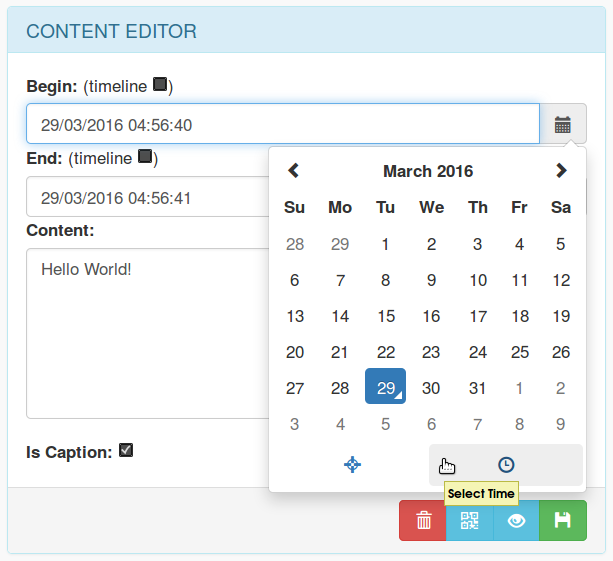
\includegraphics[width=0.6\textwidth]{figures/edition.png}
		\caption{Manual content creation}
		\label{fig:creation}
	\end{figure}


	Listing \ref{lst:createcontent} shows the structure of the content created by one user.

\begin{minipage}{\linewidth}
\begin{lstlisting}[caption={Exampe of content created by one user},label={lst:createcontent},language=json]
{
	"cmd":"createContent",
	"start":"2016-03-29T03:56:40.000Z",
	"end":"2016-03-29T03:56:41.000Z",
	"content":"<h1>Hello</h1>"
}
\end{lstlisting}
\end{minipage}
	In order to help the content creator to show and synchronize its content in real-time we allow the user to encode its content into \emph{QR codes} and show it to the camera in real time.

	\ac{KMS} lets registering event handlers for \emph{QR code} detection. The component that detects \emph{QR codes} on \ac{KMS} is called periodically and fires the handlers with the decoded content. This mechanism does not detect if the \emph{QR code} enters or leaves the screen. We had to implement our own mechanism for detecting those events.

	Each user session in the server maintains a map with the contents that are present on the screen. In order to apply our algorithm more efficiently we calculate the content's hash through the \emph{md5} method.

	If the hash is not present in the map it means the \emph{QR code} was entering the screen, we add that hash to the map and associate the current time to it, all the users are notified to watch that content in real-time. By doing an analogy to the \emph{Nyquist} theorem we know that if the same \emph{QR code} is not detected after a time bigger then two periods we can conclude that the \emph{QR code} leaved the screen and we add the correspondent content into our database. Listing \ref{lst:pseudo_qrcode} shows the pseudo code for \emph{QR code} leaving detection.

\begin{minipage}[!htb]{\linewidth}
\begin{lstlisting}[caption={Pseudo code for QR code leaving detection},label={lst:pseudo_qrcode},language=JavaScript]
var ongoingCodesMap = {};
function onCodeFound(content) {
	var startingTime = getCurrentTime() - getUserOffset();
	var hash = md5(content);
	if(ongoingCodesMap[hash] == null){
		sendQRCodeToEditingUser(hash,content);
	}
	ongoingCodesMap[hash] = startingTime;
	waitTwoSeconds(); // onCodeFound() may be called from other threads
	var newestTime = ongoingCodesMap[hash]; 
	if(newestTime == startingTime){
		var endingTime = getCurrentTime() - getUserOffset();
		ongoingCodesMap[hash] = null; 
		sendQRCodeToEditingUser(hash,null); // remove from UI
		insertContentIntoDatabase(startingTime,endingTime,content);
		sendContentToUsers(startingTime,endingTime,content);
	}
}
\end{lstlisting}
\end{minipage}


	Our main content synchronization mechanism is time based but with some programming knowledge it is possible to insert \emph{JavaScript} code that fires events on user interaction. For example, after a teacher's lecture, it is possible to show a quiz to the users in order to understand what they learned and then submit the data to the server for further analysis.


	\subsection{Synchronization}

	In our solution content is represented as simple text that can contain \ac{HTML}, \ac{CSS} or even \emph{JavaScript}, this content is displayed on defined intervals of time.

	Multiple contents can be displayed at the same time, in order to achieve that, we define layers above the video with the same size. Each layer is associated to the content.

	We have taken into account that the amount of content tends to grow with time and the user should only have access to a subset of content instead all of them, which would be very inefficient.

	The content to display for each user depends on the user's position on the time-line, this position is given by an offset between the current time and the navigated time. If the user is watching the content in real-time this offset is constant so there is no need to synchronize this value.

	Each content is divided into two components, the \emph{start} and the \emph{end} which are sent to users. The \emph{start} component contains a time stamp, the content identification number and the content itself in form of text. The \emph{end} component only contains the time stamp and the content identification number. 

	The content to return is given by the union of two content subsets:
	\begin{itemize}
		\item The intersection of the content interval and user's time.
		\item A subset of contents which starting time is immediately following the user's time.
	\end{itemize}

	The second subset is used for predicting which content the user will watch and avoid requests during its events.

	The content description messages that are sent to each user contains the constant itself on the form of a list of events and an attribute that specifies if the server has more content to return.

	Listing \ref{lst:sentcontent} shows the structure of the content sent to users.

\begin{minipage}{\linewidth}
\begin{lstlisting}[caption={Exampe of content sent to users},label={lst:sentcontent},language=json]
{
	"cmd":"content",
	"data":[{
			"id":"56f9fd1aa986c615fab43d69",
			"time":"2016-03-29T03:56:40.000Z",
			"type":"start",
			"content":"<h1>Hello</h1>"
		},{
			"id":"56f9fd1aa986c615fab43d69",
			"time":"2016-03-29T03:56:41.000Z",
			"type":"end"
		}
	],
	"more":false
}
\end{lstlisting}
\end{minipage}

	When a user enters the conference room, immediately after the \emph{WebSocket} creation the server sends him the current content.

	The user receives the content, sorts all components by time and creates a set of events. All the events before the user's time are rendered and removed from the set of events. A timer is scheduled for the first component on the event set and the process repeats while the set is not empty.

	If the set is empty, there two options, if the server contained more content a new request for content is made and the process starts from the beginning, namely the server sends the correspondent content again. If the server has no more content the process is stopped until it sends more.

	The users will receive their contents from the server on five different situations:

	\begin{itemize}
		\item Conference room entrance (advertised by server).
		\item Set of events empty and server has more content (client requested).
		\item Content is created (advertised by server).
		\item Content is removed (advertised by server).
		\item User navigates to different point in time (client requested).
	\end{itemize}



	Listing \ref{lst:pseudo_render} presents the pseudo code for our content scheduler.

\begin{minipage}[!htb]{\linewidth}
\begin{lstlisting}[caption={Pseudo code for hyper content scheduler},label={lst:pseudo_render},language=JavaScript]
function scheduleContent() {
    var navigatedTime = getCurrentTime() - getUserOffset();
    while ( hasLocalEvents() ) {
        if ( firstEventIsOlderThanNavigatedTime() ) {
            if ( firstEventIsStart() ) {
            	addHtmlLayer(event);
            } else {
            	removeHtmlLayer(event);
            }
            removeFirstEvent();
        } else {
            break;
        }
    }
    if ( hasNoLocalEvents() ) {
    	return;	// nothing to do
    } 
    if ( hasNoStartEvents() && serverHasMoreContent() ) { 
       	requestContentFromServer(navigatedTime);
    } else {
        waitUntilNextEvent();
        scheduleContent();
    }
}
\end{lstlisting}
\end{minipage}

	\subsection{Security Concerns}

	Our solution is flexible on what kind of interactions are possible to the users in real time but allowing users to write \emph{JavaScript} that is executed on the other users browser would attackers to misuse their resources and access to critical information.

	We could solve this problem easily by escaping any \emph{script} tag present on the content, but we would sacrifice the kind of interactions that are possible. 

	By not allowing \emph{JavaScript} we would need to implement all actions a priori and fire them when a type of message is received. We decided to ignore the security vulnerabilities that are exposed by evaluating \emph{JavaScript} because in order to offer the same interactions we would have to do an exhaustive functional requirements gathering.

	Another way to solve this problem, which is not within the goals of this thesis, is to analyze the \emph{JavaScript} code and detect if it is malicious.

	\subsection{Time Manipulation}

	We have used \emph{vis.js} to display out time-line. This library was created for content navigation through time, but it was not designed to be always moving automatically, we have created a background timer that performs the animation of moving the window of time bounds and user navigated time marker.

	Figure \ref{fig:timeline} shows the the graphic appearance of our interactive time-line, in order to navigate through time the user must drag and drop the time-line horizontally, when the user drops the time-line an event handler is called with the new user's time offset which will be used to send a message to the server in order to choose the correspondent content to display. 

	\begin{figure}[!htb]
		\centering
		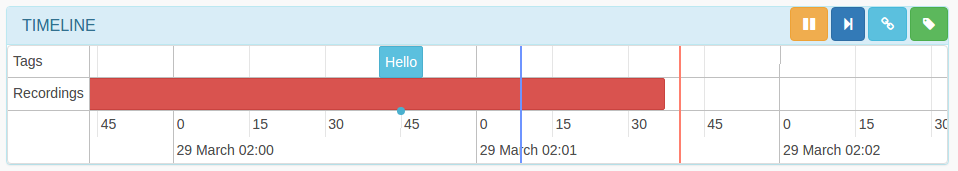
\includegraphics[width=\textwidth]{figures/timeline.png}
		\caption{Interactive time-line}
		\label{fig:timeline}
	\end{figure}

	We have noticed the server time being different from client time and this created graphic inconsistencies such as showing existing recorded blocks of movie in the future. To solve this problem the server sends its time to client immediately after the \emph{webSocket} creation, we synchronize the time-line with the server and although it may exist a small error due to network transmission time the graphical error is negligible. 


	\subsection{Time annotations creation}

	Time annotations are simpler way save points in time and share them with other users. When a user enters in a conference room the server sends all annotations so they can be displayed directly into the user time-line. Each time annotation is created all users are advertised so they can update their interfaces.

	Figure \ref{fig:annotation} shows the creation and placement of annotations on the time-line, to save the annotation the user must click on the floppy icon in order to save it and advertise the conference participants. 

	\begin{figure}[!htb]
		\centering
		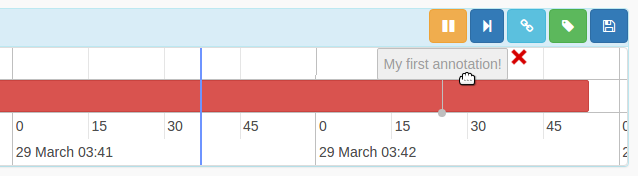
\includegraphics[width=0.7\textwidth]{figures/annotation.png}
		\caption{Creating a time annotation}
		\label{fig:annotation}
	\end{figure}

	Besides the ability to create tags it is also possible to create time hyper-links, see figure \ref{fig:timelink}, that can be sent to other users externally so they can navigate directly to the content when entering in the conference room.


	\begin{figure}[!htb]
		\centering
		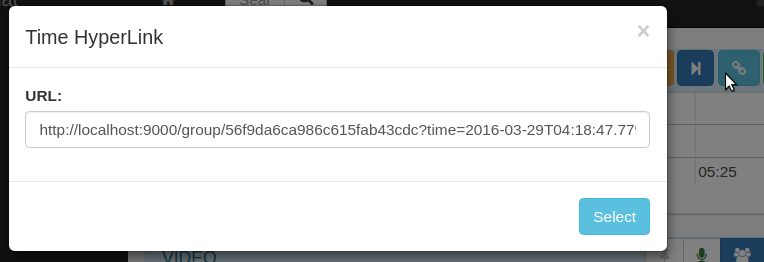
\includegraphics[width=0.8\textwidth]{figures/timelink.png}
		\caption{Time link creation}
		\label{fig:timelink}
	\end{figure}


	\subsection{Content Search}

	Users can easily search for annotations and contents and travel to their correspondent times. In the case of hyper content after handling the result from database we ignore \ac{HTML} tags, extract the text with \emph{Jsoup}\footnote{\url{http://jsoup.org/} (Accessed 21 March 2016)} and apply the query again. We extract the text from \ac{HTML} because accidentally searching for text contained in \ac{HTML} tags would lead to incorrect results.

	Figure \ref{fig:search} shows how the search results are displayed to the user. Each result entry contains an icon specifying the type of result (hyper content, time annotation, ...).




\begin{figure}[!htb]
\centering
\begin{minipage}[b]{0.55\linewidth}
\centering

		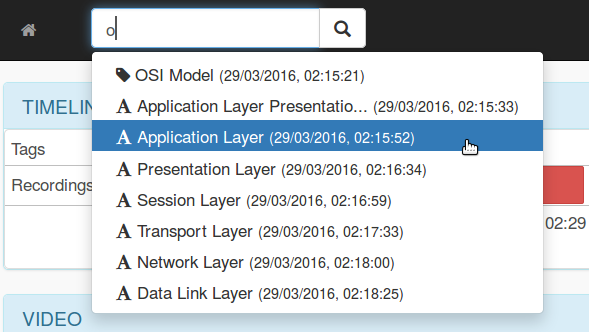
\includegraphics[width=\textwidth]{figures/search.png}
	      a) Result list
\label{fig:minipage1}
\end{minipage}
\quad
\begin{minipage}[b]{0.40\linewidth}
		\centering

		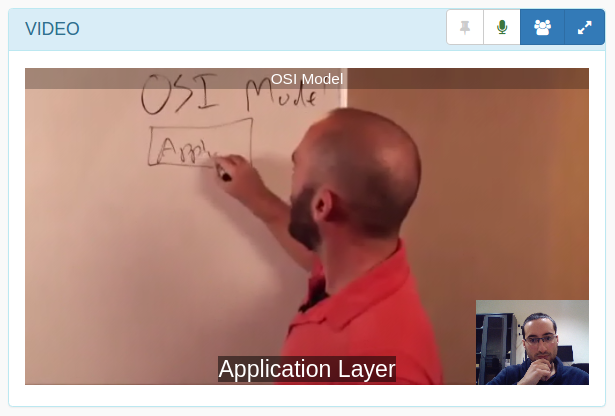
\includegraphics[width=\textwidth]{figures/search2.png}
	       b) Selected result
\label{fig:minipage2}
\end{minipage}

		\caption{Example of search results}
		\label{fig:search}
\end{figure}

	\subsection{Switching views}

		We provide a way for users to select the composite view of the conference room or the video shared by a particular user device as it can be seen on figure \ref{fig:devices}. 

		In order to maintain a list of available user devices that can be played at the navigated time if a user plays or ends playing a block of recorded video it obtains at the same time a list of all devices available for each user at that time.

		On the other hand, if a user changes to real time, the list of devices is extracted from the set of \emph{webSockets} that are associated to the respective conference room. This list of devices is also sent to the users that are also in real time mode whenever a new user enters or leaves the conference room.

	\begin{figure}[!htb]
		\centering
		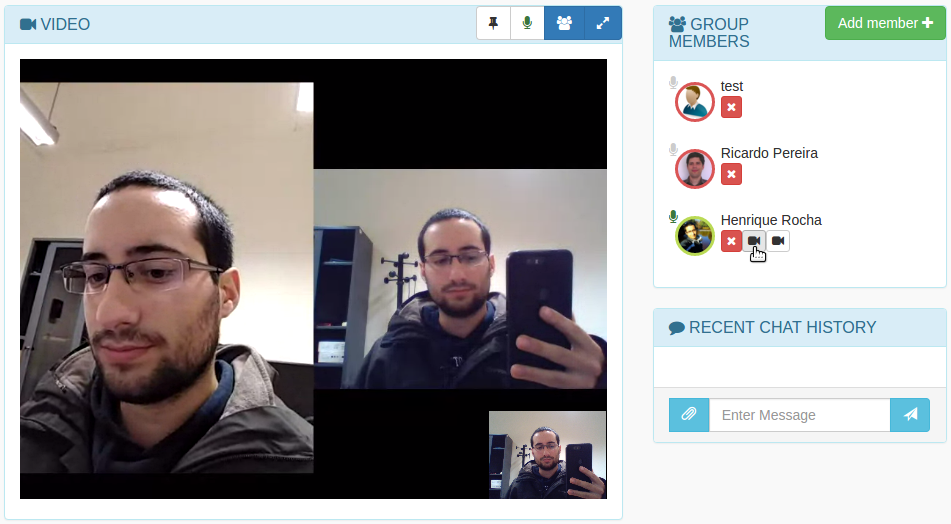
\includegraphics[width=0.8\textwidth]{figures/devices.png}
		\caption{Multiple devices per user}
		\label{fig:devices}
	\end{figure}

		We also provide an automatic mechanism for switching the view to the current speaker. With respect to sound analysis, the sound samples are analyzed on the client side through the web audio \ac{API}.

		Our speech detector is straightforward, we could perform a spectral analysis in order to understand if the analyzed sound contains frequencies in the range of the human voice but instead we just capture sound samples in real time and calculate the maximum sound amplitude. If a sound sample has an amplitude bigger than a factor of the maximum amplitude (we have used an empirical value of 10\%) we say that the user is speaking and therefore we send a message to the server if the speaking state has changed. Subsequently, the server receives the user speaking state and sends it to the other users so they can request a different view.

\chapter{Evaluation}
\label{chapter:evaluation}
  In the previous chapter we described how we implemented our solution namely the data model that we used, the description of the signaling protocol, how we performed stream recording, how we overlayed interactive content to video and lastly how we deployed our solution. 

  In this chapter we describe how we tested our solution, show and analyze the results in order to validate the contributions of this thesis.

\section{Tests Objectives}

  We have tested our solution with real users for a better understanding of their difficulties and what can be done in order to improve our solution's usability.

  We have also tested the performance of our solution by measuring the used resources. Those performance tests are crucial to ensure that our solution is in fact stable and users can use it timelessly without decreasing the quality of their experience. 


  \section {Performance Tests}

     In this section we describe performance test scenarios that we have applied and their respective results.


    \subsection{Tests Scenarios}


      In order to benchmark our system, we have implemented a small \emph{Python} script using \emph{psutil}\footnote{\url{https://github.com/giampaolo/psutil} (Accessed March 27, 2016)} that collects with a periodicity of one second; CPU, physical memory information relative to each running process and network usage relative to each interface. 

      We would like to collect network information relative to each process, which \emph{nethogs}\footnote{\url{https://raboof.github.io/nethogs/} (Accessed March 27, 2016)} provide but it could not capture the network usage of some processes. Although this would be useful for a deep analysis, we know which network interfaces are used to establish connections between processes as we show on table \ref{table:interfacemap}.

  \begin{table}[!htb]
\centering
\caption{Mapping of connections by network interface}
\label{table:interfacemap}
\begin{tabular}{|l|l|}
\hline
\multicolumn{1}{|c|}{\textbf{Interface}} & \multicolumn{1}{c|}{\textbf{Connection}}         \\ \hline
Loopback & Web Server $\leftrightarrow$ MongoDB  \\ \hline
Loopback & Web Server $\leftrightarrow$ Kurento Media Server  \\ \hline
Loopback & Kurento Media Server $\leftrightarrow$ Kurento Repository $\leftrightarrow$ MongoDB  \\ \hline
Ethernet & Web Server $\leftrightarrow$ Client\\ \hline
Ethernet & Kurento Media Server $\leftrightarrow$ Client\\ \hline
\end{tabular}
\end{table}


      The performance test scenario that we have defined consists on two phases, the first phase consists only on having users, with similar computer and network specifications, entering sequentially on the conference room, the second phase consists on the users leaving the conference room. Each event, joining and leaving, occurs with intervals of one minute in total of thirteen minutes (780 seconds).

  


\subsection{Test Results}
  
      We are presenting in this section the results of our performance tests after implementing our solution.
\subsubsection{Network usage}

      Every time a user shares its camera or its screen in the context of a conference room, its offered video is sent to the server and independently from watching an individual stream or the mixed version the server just sends a unique stream back to the user.

      From the media server prespective if there are $n$ clients connected each of them sending and receiving one stream, it is expected that server sends and receives also $n$ streams. By so we expect that the amount of network increases linearly as users join a conference room.

      Figure \ref{fig:test_full_features_net} confirms our expectations, each vertical yellow line represents each event, the first seven events are users entering the conference room the next ones represent users leaving the conversation. 
      

\begin{figure}[!htb]
  \centering
  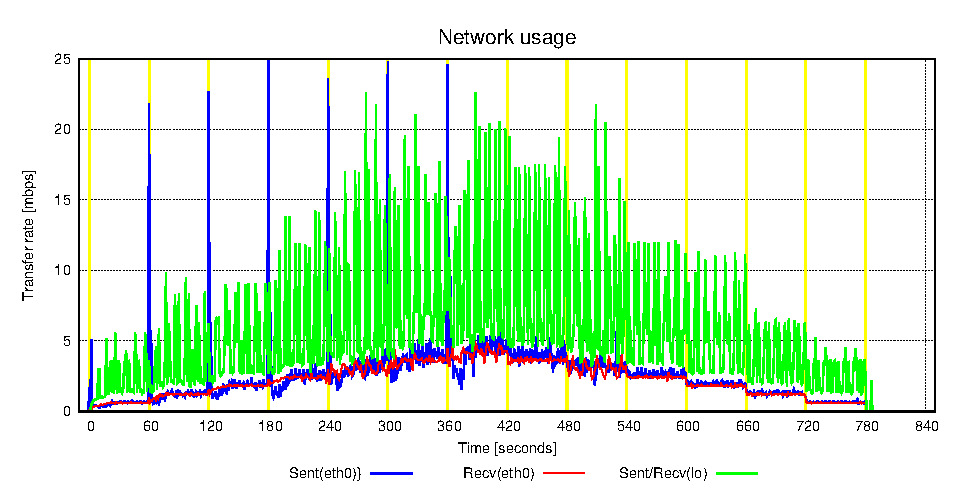
\includegraphics[width=\textwidth]{stats/test_full_features_net.eps}
  \caption{Network usage after implementing all features}
  \label{fig:test_full_features_net}
\end{figure}


      The blue peaks are caused by the signaling phase and web page downloads, including resources such as images, stylesheets and javascript files. 
      The green peaks are caused by that being transfered between \ac{KMS} and \emph{MongoDB} through \emph{Kurento Repository} each peak occurs each time a block of video is recorded which in this case is every ten seconds. 
      The recordings are synchronized so all user and mixed blocks starts and ends at the same time, that's why the amount of work done every ten seconds accumulates and because this is performed locally the maximum transfer rate is limited by the performance of the memory as buffers are written to buffers then to disks. 
      Client's sent data transfer rate has no significant peaks as signaling information contains few information.

      Figure \ref{fig:summary_full_net} shows the average transmission rate per interval of consecutive events. 


\begin{figure}[!htb]
  \centering
  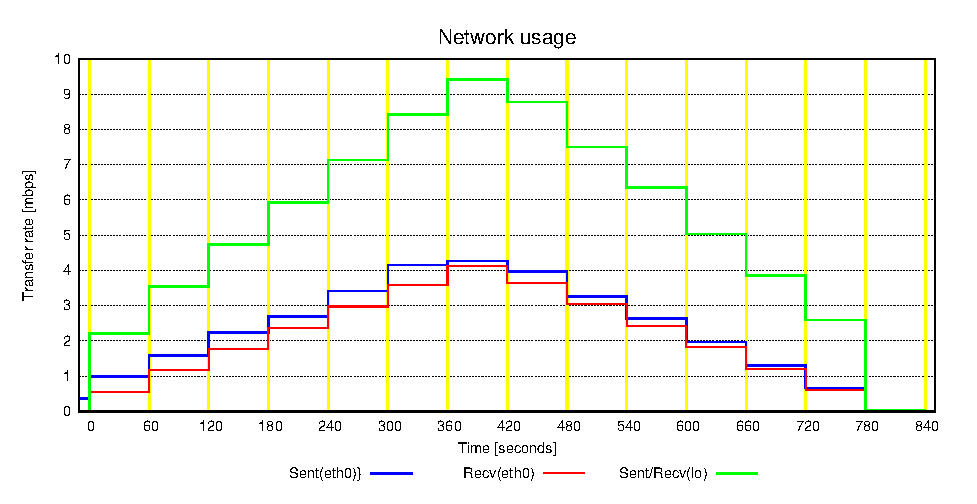
\includegraphics[width=\textwidth]{stats/summary_full_net.eps}
  \caption{Average network usage per interval of events after implementing all features}
  \label{fig:summary_full_net}
\end{figure}



If we consider all streams equal and an incoming stream uses $x$kbps, with $n$ incoming streams the rate of data received at \ac{KMS} is $nx$ and the expected rate of data transfered to \emph{Kurento Repo} using localhost is $(n+1)x$. Due to the data being transfered also from \emph{Kurento Repo} to \emph{MongoDB} via localhost, the expected total rate of data transfered through localhost is $2((n+1)x) = (2n+2)x$, which explains the reason for the average amount of data transfered through localhost being more than twice the average amount of data received from users.

With this results we conclude that if we want to scale our solution's storage using the \emph{MongoDB}'s cluster configuration, both \emph{Kurento Repository} and \emph{MongoDB} should be installed in the same machine because the loopback interface can handle bigger transfer rates than the remaining network interfaces. For the same reason another possible configuration for scaling the storage is to install both \emph{Kurento Repository} and \ac{KMS} on the same machine.

On the other hand figure \ref{fig:test_client_net} shows the respective network usage on the client side during our test case. We observe that int he first seconds the client adjusts the video quality that sends to \ac{KMS}, whenever a new client enters in the conference we observer that \ac{KMS} decreases the video quality in order to instantaneously integrate a new user into the conference room, after a while \ac{KMS} realizes that its network can handle the increase of clients and sends the video with a better quality to every participant. When a user leaves the conference room \ac{KMS} has no need to decrease the participant's video quality as less network bandwidth will be used.

\begin{figure}[!htb]
  \centering
  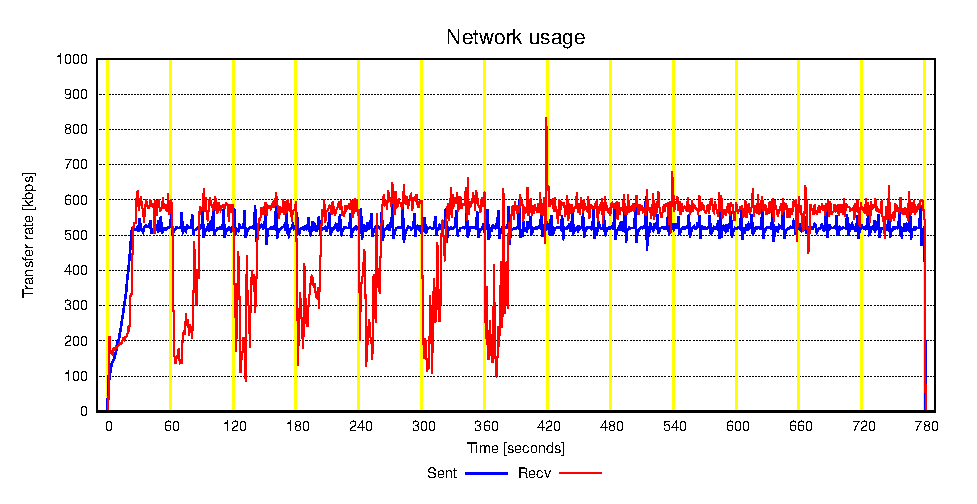
\includegraphics[width=\textwidth]{stats/test_client_net.eps}
  \caption{Client Network usage during our test case}
  \label{fig:test_client_net}
\end{figure}



\subsubsection{Memory usage}


Figure \ref{fig:test_full_features_mem} shows the memory usage during our performance test case. Both \ac{JVM}, \emph{MongoDB} and \ac{KMS} performs their own memory management by holding and recycling objects when needed. The expected and observed behavior of the memory usage is growth memory usage while the users are entering in the conference room and a memory usage stabilization afterwards.



\begin{figure}[!htb]
  \centering
  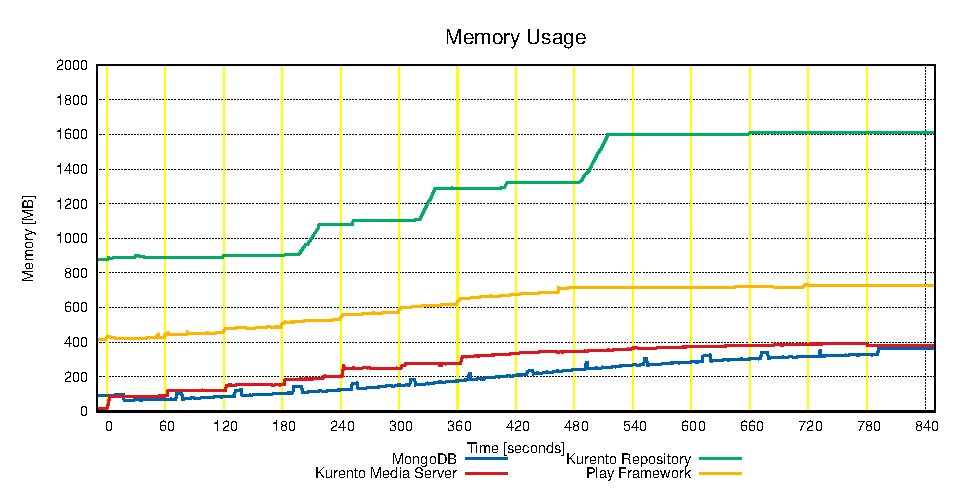
\includegraphics[width=\textwidth]{stats/test_full_features_mem.eps}
  \caption{Memory usage after implementing all features}
  \label{fig:test_full_features_mem}
\end{figure}


\emph{MongoDB} memory usage keeps increasing because it tries to fit part of the database on \ac{RAM} for fast read access. \emph{MongoDB} checkpoints data to disk every 60 seconds or when journal data exceeds 2GB\footnote{\url{https://docs.mongodb.org/manual/faq/storage/}(Accessed March 28, 2016)}, that explains the small memory usage peaks during our test case. When the conference room is empty no there are no video recordings, which explains the memory stabilization at the end.

\emph{KMS} memory usage was increasing and in fact we did not expected that, we have done more tests and we have observed that by disabling the recorder feature memory usage kept linearly related to the amount of clients present on the room. Therefore, we have verified our implementation and we have concluded that nothing was wrong with our code, we have confirmed that every allocated resource was indeed released after the end of recording. As a result of our intensive tests and consecutive failures we suspected that the problem was not ours.

Hence, in order to confirm our suspicions, we have decided to read the implementation of \ac{KMS} and we have found that \ac{KMS} was not releasing the memory if the recorder was stopped by us. Subsequently, we have changed the source code and submitted to \emph{Kurento} team through a \emph{GIT}'s \emph{"pull request"}.


Figure \ref{fig:test_ram_fixed_mem} shows the memory usage during our performance test case taking into account the patch that we applied to \ac{KMS}.



\begin{figure}[!htb]
  \centering
  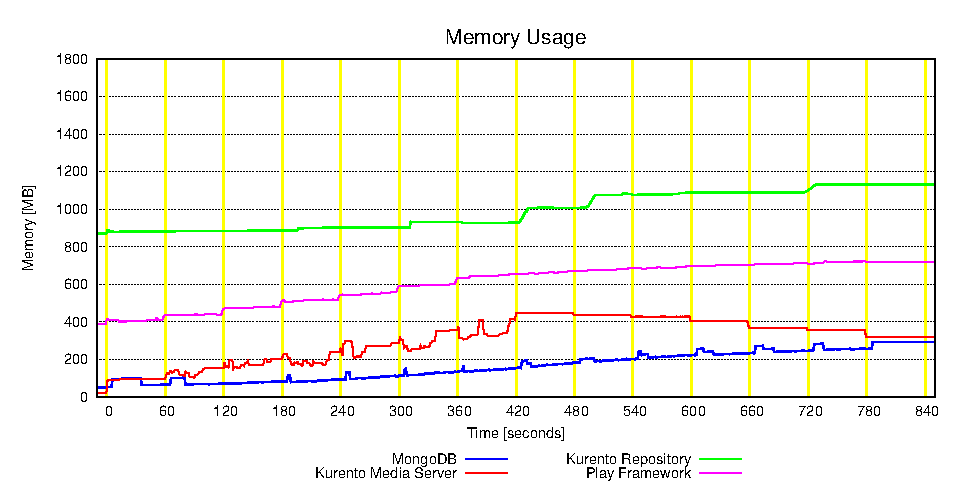
\includegraphics[width=\textwidth]{stats/test_ram_fixed_mem.eps}
  \caption{Memory usage after fixing recorder memory leak}
  \label{fig:test_ram_fixed_mem}
\end{figure}


\subsubsection{CPU usage}


Figure \ref{fig:test_full_features_cpu} shows the percentage of \ac{CPU} usage during our performance test case. Each 100\% represents one \ac{CPU} core, although that does not mean one \ac{CPU} is fully used, for example two cores at 60\% represent 120\% \ac{CPU} usage. As we can see, the percentage of \ac{CPU} used increases and decreases linearly in function of the amount of conference participants. 

\begin{figure}[!htb]
  \centering
  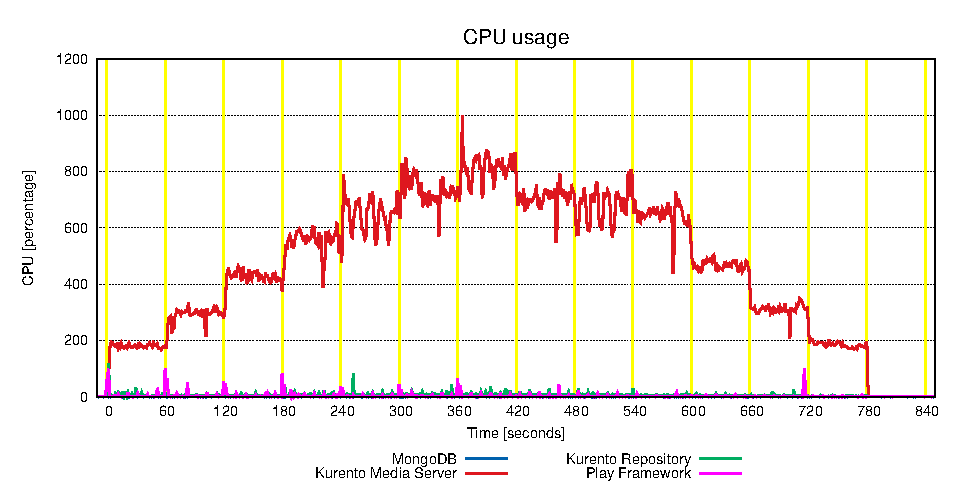
\includegraphics[width=\textwidth]{stats/test_full_features_cpu.eps}
  \caption{Percentage of CPU used during the performance tests}
  \label{fig:test_full_features_cpu}
\end{figure}

Figure \ref{fig:test_full_features_cpu_zoom} is the same as figure \ref{fig:test_full_features_cpu} but zoomed over \emph{MongoDB}, \emph{Java} and \emph{Kurento Repository}. As we can see there are periodic processing peaks every ten seconds that are due to block recording. 

\begin{figure}[!htb]
  \centering
  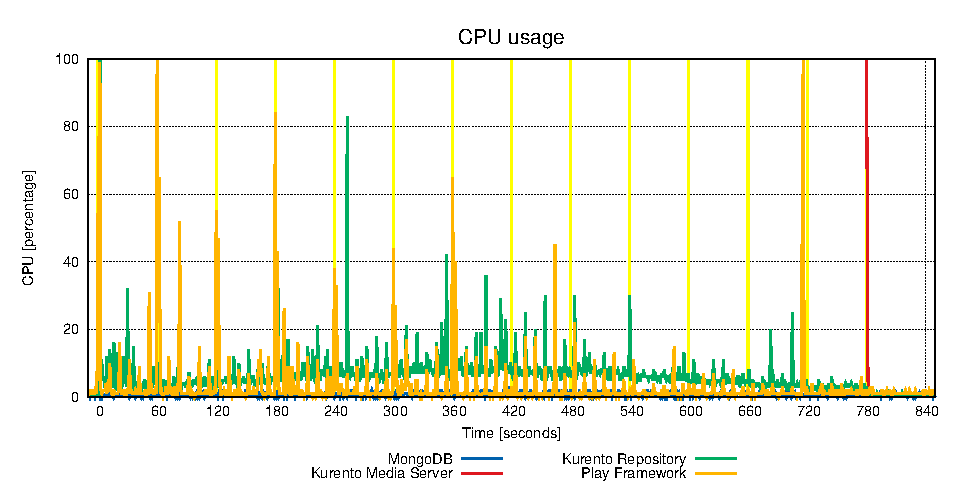
\includegraphics[width=\textwidth]{stats/test_full_features_cpu_zoom.eps}
  \caption{Percentage of CPU used during the performance tests (zoomed)}
  \label{fig:test_full_features_cpu_zoom}
\end{figure}


   Figure \ref{fig:summary_full_cpu} shows the average used \ac{CPU} per interval of consecutive events. 

\begin{figure}[!htb]
  \centering
  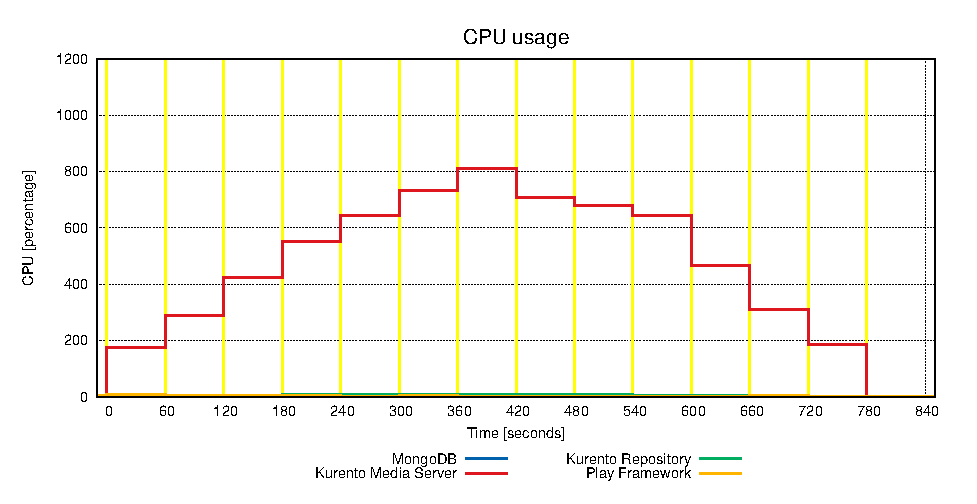
\includegraphics[width=\textwidth]{stats/summary_full_cpu.eps}
  \caption{Average percentage of CPU used per interval of events after implementing all features}
  \label{fig:summary_full_cpu}
\end{figure}



  Just for testing purposes we have done the same performance tests without detecting \emph{QR codes} in order to understand how \ac{CPU} intensive is this task. Figure \ref{fig:test_without_qrcode_cpu} shows the results for the same experience but with \emph{QR code} detection disabled.

\begin{figure}[!htb]
  \centering
  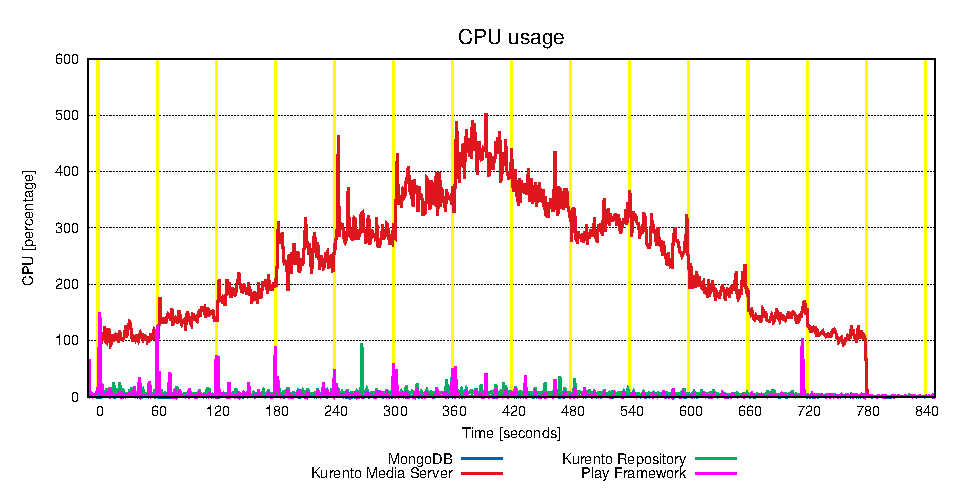
\includegraphics[width=\textwidth]{stats/test_without_qrcode_cpu.eps}
  \caption{Percentage of CPU used during the performance tests without QR code detection}
  \label{fig:test_without_qrcode_cpu}
\end{figure}

We conclude that \emph{QR code} detection is a very intensive task, approximately doubling the amount of work performed by \ac{CPU}. Without this feature the network and memory usage had insignificant changes compared to \ac{CPU} usage.

\subsubsection{Two consecutive test cases}


We have also performed two consecutive test cases in order to understand if we the influence of the first test case over the second, as observed in figure \ref{fig:test_two_times_cpu}, there is no \ac{CPU} influence between two test cases.


\begin{figure}[!htb]
  \centering
  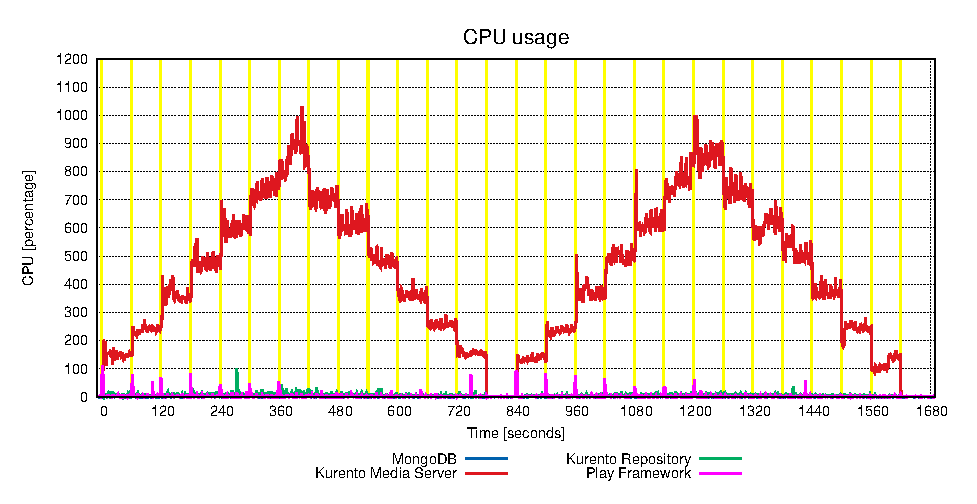
\includegraphics[width=\textwidth]{stats/test_two_times_cpu.eps}
  \caption{Percentage of CPU used during two consecutive test cases}
  \label{fig:test_two_times_cpu}
\end{figure}

On the other hand due to memory recycling techniques we can observe in figure \ref{fig:test_two_times_mem} that some of the memory that was allocated in the first test was reused in the second case.


\begin{figure}[!htb]
  \centering
  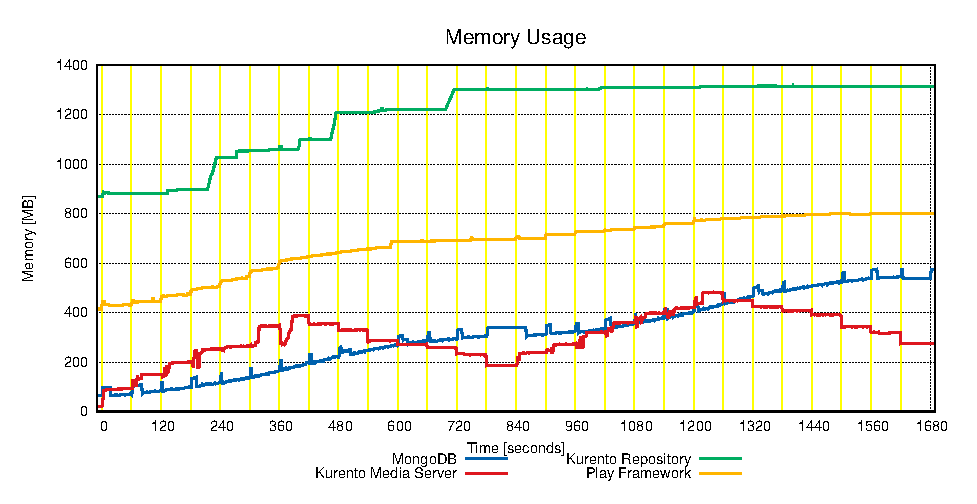
\includegraphics[width=\textwidth]{stats/test_two_times_mem.eps}
  \caption{Memory usage during two consecutive test cases}
  \label{fig:test_two_times_mem}
\end{figure}


\subsubsection{One hour test case}


   Figure \ref{fig:test_hour_mem} shows the memory used by our solution with seven clients simultaneously on the same conference room during one hour. As we can observe \ac{KMS} memory usage stabilizes.


\begin{figure}[!htb]
  \centering
  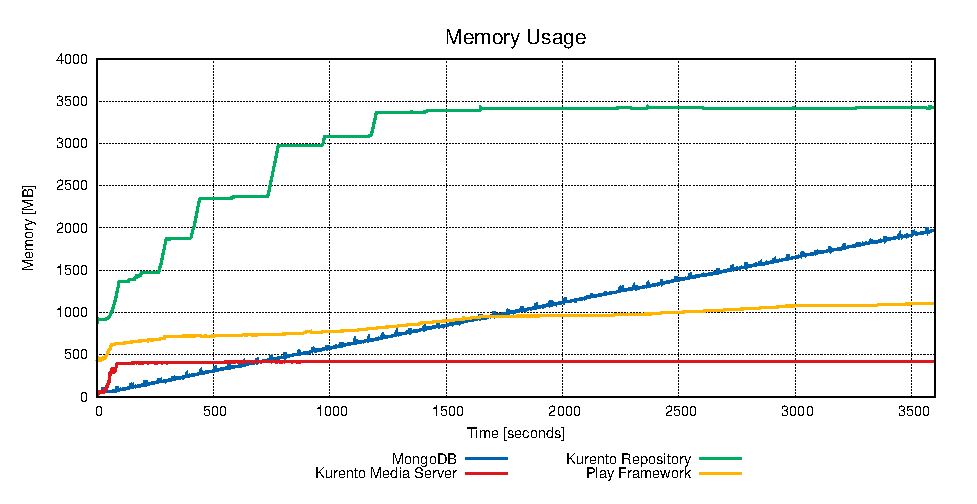
\includegraphics[width=\textwidth]{stats/test_hour_mem.eps}
  \caption{Memory usage during one hour with seven clients}
  \label{fig:test_hour_mem}
\end{figure}





\section {Usability Tests}
     In this section we describe usability test scenarios that we have applied and their respective results.


    \subsection{Tests Scenarios}

      In order to the usability of our solution, we haver performed usability tests with the help of real users with different backgrounds and ages.

      We handled a guide to the users with five tasks to perform, the metrics we used for each task were: number of clicks, number of errors including a description and time spent. 

      The tasks we asked to the user are:

      \begin{enumerate}
      \item Login into the system with the provided credentials and accept the received friendship request. Find the coordinator's brother and add him as a friend.

      \item Create a private conference room, enter and share your screen, add the coordinator to the conference room and chat with him. After that use the collaborative editor in order to write at the same time as the coordinator. Lastly save the editor and leave the conference room.

      \item Enter in the conference room correspondent to the third task as an observer and navigate to the specified annotation. Watch the video until a list of topics is overlayed in the video and choose one of them and leave the conference room.

      \item Enter in the conference room correspondent to the fourth task by sharing your camera and create a time annotation in the instant of time when you entered, navigate to the current time, search for the annotation and leave the conference room.

      \item Enter in the conference room correspondent to the fourth task by sharing your camera and add a subtitle in the video, preview it, specify an interval of time and save it. Then show the provided \emph{QR code} to the camera and leave the leave the conference room.
      \end{enumerate}

      The goal of the first task consists on evaluating the interface for authentication and friendship management.

      The second task is used to make the users familiar with our tools for collaborative content edition.

      The goal of the third task is to demonstrate the navigation functionalities and synchronized interactive content superposition.

      The fourth task is used to analyse the behavior and difficulties of the user when creating a time annotation.

      The goal of the fifth task is to create synchronized overlayed content, demonstrate the difficulties of such task and present an easier way to synchronize content.

  \subsection{Test Results}

In this section we present the results of our usability tests. The first time we tested our solution by providing tasks to users, we have observed that our solution was not perfect. We have faced usability problems during our tests, he had to improve our solution's usability and start the tests again.

  \subsubsection {First phase}

In the first testing phase we have performed just three tests with users and ceased for improvements. 

Both users that tested our solution had difficulties on the first task when finding new friendship requests and adding new friends, as friendship request were possible to access only from the top bar and new user profiles were only accessible through the search bar. In order to solve this problem we have added a menu for adding new users in the friends list and another near the friends list as it can be seen on figure \ref{fig:test_ui_01_02_03}.

\begin{figure}[!htb]
\centering
\begin{minipage}[b]{0.2\linewidth}
\centering

    
\includegraphics[width=\textwidth]{figures/test_ui_01.png}
        a) Friend list path
\label{fig:minipage1}
\end{minipage}
\begin{minipage}[b]{0.35\linewidth}
    \centering

    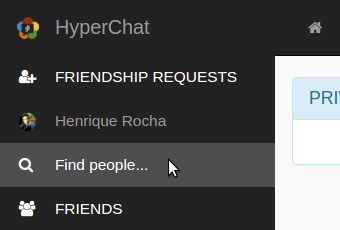
\includegraphics[width=\textwidth]{figures/test_ui_02.png}
         b) Friend requests path
\label{fig:minipage2}
\end{minipage}
\begin{minipage}[b]{0.2\linewidth}
    \centering

    
\includegraphics[width=\textwidth]{figures/test_ui_03.png}
         c) Search bar path
\label{fig:minipage2}
\end{minipage}

    \caption{Multiple paths for finding people}
    \label{fig:test_ui_01_02_03}
\end{figure}

On the second task one user clicked on the friends list for adding a friend to room and by consequence made him leave the conference room to the user profile. We solved this problem by showing a pop-up with the user profile and an additional button to add the user to the conference room as it can be seen on figure \ref{fig:test_ui_04}.

\begin{figure}[!htb]
\centering
\begin{minipage}[b]{0.7\linewidth}
\centering

    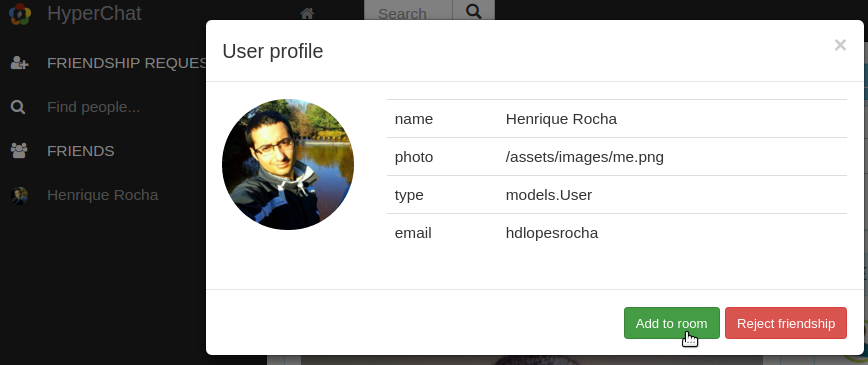
\includegraphics[width=\textwidth]{figures/test_ui_04.png}
\end{minipage}


    \caption{Adding user to conference room from user profile}
    \label{fig:test_ui_04}
\end{figure}

On the third task we noticed that both users were not expecting to search the content directly from the search bar, instead they used the time-line.

On the fourth task both users didn't placed their annotations on right place, we only provide one way to place annotations, which is by dragging them on the time-line. 
After creating an annotation users also didn't understand that they had to save their changes on the time-line, we solved this problem by saving automatically each time the user changed any annotation, the old user interface can be seen on figure \ref{fig:test_ui_05}.

\begin{figure}[!htb]
\centering
\begin{minipage}[b]{0.3\linewidth}
\centering

    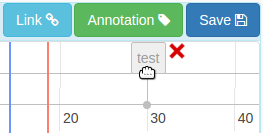
\includegraphics[width=\textwidth]{figures/test_ui_05.png}
\end{minipage}


    \caption{Save button that was removed}
    \label{fig:test_ui_05}
\end{figure}

Both users had success with fifth task but they revealed difficulties choosing the time interval for the hyper content, we are aware that this is a difficult task and that's why we have introduced the \emph{QR code} content creation mechanism which was very easy to learn.

We have also gathered comments and suggestions after letting the users explore our system, extra improvements were made such as:

\begin{itemize}
\item Giving feedback to user when saving content and collaborative editors.
\item Support file upload on our chat.
\item Starting with our time-line more zoomed in order to give more sensation of time.
\item Create content with starting time and duration instead ending time.
\end{itemize}

  \subsubsection {Second phase}

On the second phase of our user interface tests, in a general view, we have noticed great improvements on the learning time.

From the data that we have collected, namely the task duration (figure \ref{fig:user_times}), number of clicks (figure \ref{fig:user_clicks}), number of errors (figure \ref{fig:user_errors}), task difficulty (figure \ref{fig:user_diffs}) and qualitative evaluation (figure \ref{fig:user_evals}), we have calculated the confidence intervals in order to understand the most plausible values for each metric.

As a result of both true average and variance being unknown and the usage of a relatively small amount of samples, we had to use \emph{t-distribution} to estimate our metrics confidence intervals. 

Accordingly, we have used the following formula to calculate the intervals for the expected value of the true average with 95\% confidence:
\begin{equation}
[\bar{x}-F^{-1}_{t_{(n-1)}}(1-\alpha/2)\times \frac{s}{\sqrt{n}}, \bar{x}+F^{-1}_{t_{(n-1)}}(1-\alpha/2)\times \frac{s}{\sqrt{n}}]
\end{equation}

Where $\alpha=0.05$, $n$ is the number of samples (which may not coincide with the number of tests due to failed tasks), $\bar{x}$ is the sample mean, $x_i$ is the sample value and $s$ is the sample standard deviation that is given by:
\begin{equation}
s=\sqrt{\frac{1}{n-1}\Sigma^{n}_{i=1}(x_i-\bar{x})^2}
\end{equation}

\begin{figure}[!htb]
\centering
\begin{minipage}[b]{0.45\linewidth}
  \begin{center}
    
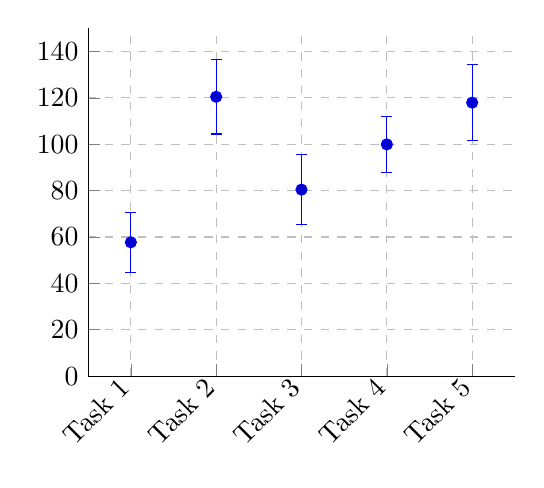
\begin{tikzpicture}[scale=1.0],
\centering
\begin{axis}[
height=6cm,
width=7cm,  
  ymax=150,
  ymin=0,
  xmin=0.5,
  xmax=5.5,
  axis y line*=left,
  axis x line*=bottom,
  xticklabels={Task 1,Task 2,Task 3,Task 4,Task 5},
  xtick={1,...,5},
  ytick={0,20,...,200},
        ymajorgrids=true,
      xmajorgrids=true,
      grid style=dashed,
  x tick label style={rotate=45,anchor=east}]
\addplot+[only marks][error bars/.cd,y dir=both, y explicit]
coordinates {
(1,57.7) +- (12.827,12.827)
(2,120.44) +- (16.041,16.041)
(3,80.409) +- (15.067,15.067)
(4,99.91) +- (11.948,11.948)
(5,117.92) +- (16.31,16.31)
};
\addplot[dashed] coordinates {(0,0) (5.5,0)};
\end{axis}
\end{tikzpicture}%

  \end{center}
  \caption{Time spent per task}
  \label{fig:user_times}
\end{minipage}
\begin{minipage}[b]{0.45\linewidth}
   \begin{center}
    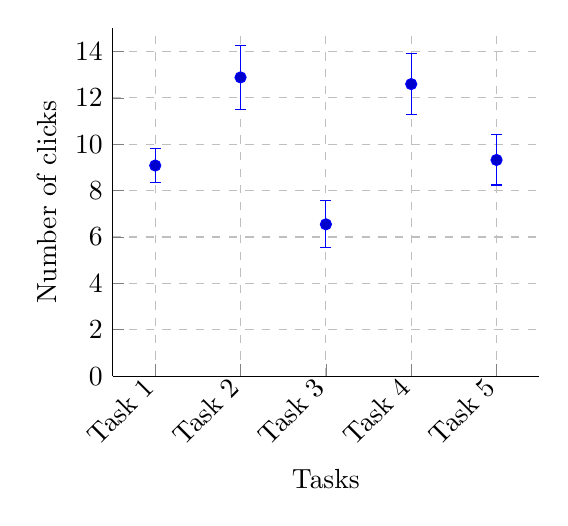
\begin{tikzpicture}[scale=1.0],
\centering
\begin{axis}[
height=6cm,
width=7cm, 
  xlabel={Tasks},
  ylabel={Number of clicks}, 
  ymax=15,
  ymin=0,
  xmin=0.5,
  xmax=5.5,
  axis y line*=left,
  axis x line*=bottom,
  xticklabels={Task 1,Task 2,Task 3,Task 4,Task 5},
  xtick={1,...,5},
  ytick={0,2,...,200},
        ymajorgrids=true,
      xmajorgrids=true,
      grid style=dashed,
  x tick label style={rotate=45,anchor=east}]
\addplot+[only marks][error bars/.cd,y dir=both, y explicit]
coordinates {
(1,9.08) +- (0.731,0.731)
(2,12.88) +- (1.3855,1.3855)
(3,6.5455) +- (1.0107,1.0107)
(4,12.591) +- (1.3126,1.3126)
(5,9.32) +- (1.0793,1.0793)
};
\addplot[dashed] coordinates {(0,0) (5.5,0)};
\end{axis}
\end{tikzpicture}%
  \end{center}
  \caption{Mouse clicks per task}
  \label{fig:user_clicks}
\end{minipage}
\end{figure}


Accordingly to figure \ref{fig:user_evals}, we can observe that most users had less difficulties with the first two tasks, which represents types of tasks that most users are familiar with. As soon as users had to navigate in time, manipulate annotations and create content (respectively \emph{task3}, \emph{task4} and \emph{task5}) we have observed that they revealed more difficulties. Most of those difficulties, based on the users feedback, were mainly due to those concepts not being familiar to them.

\begin{figure}[!htb]
\centering
\begin{minipage}[b]{0.45\linewidth}
  \begin{center}
    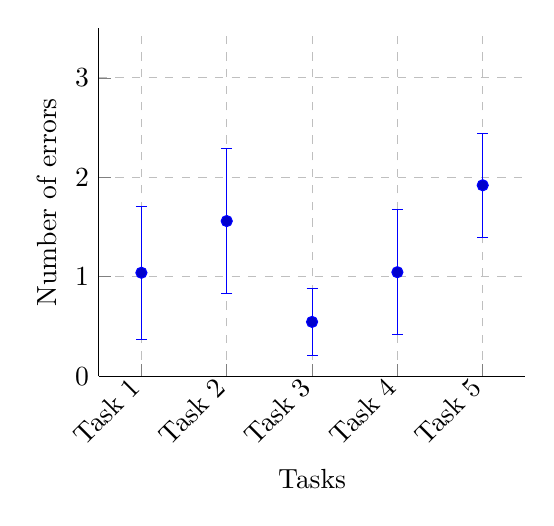
\begin{tikzpicture}[scale=1.0],
\centering
\begin{axis}[
height=6cm,
width=7cm,  
  xlabel={Tasks},
  ylabel={Number of errors}, 
  ymax=3.5,
  ymin=0,
  xmin=0.5,
  xmax=5.5,
  axis y line*=left,
  axis x line*=bottom,
  xticklabels={Task 1,Task 2,Task 3,Task 4,Task 5},
  xtick={1,...,5},
  ytick={0,1,...,20},
  ymajorgrids=true,
  xmajorgrids=true,
  grid style=dashed,
  x tick label style={rotate=45,anchor=east}]
\addplot+[only marks][error bars/.cd,y dir=both, y explicit]
coordinates {
(1,1.04) +- (0.668,0.668)
(2,1.56) +- (0.728,0.728)
(3,0.5455) +- (0.3365,0.3365)
(4,1.0455) +- (0.6283,0.6283)
(5,1.92) +- (0.5215,0.5215)
};
\addplot[dashed] coordinates {(0,0) (5.5,0)};
\end{axis}
\end{tikzpicture}%
  \end{center}
  \caption{Errors per task}
  \label{fig:user_errors}
\end{minipage}
\begin{minipage}[b]{0.45\linewidth}
  \begin{center}
    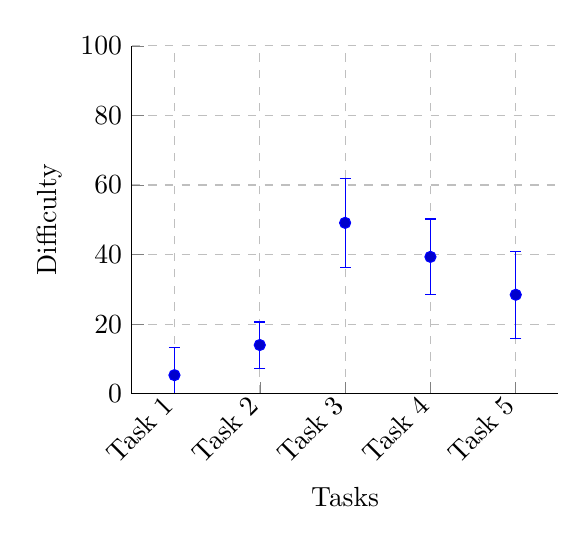
\begin{tikzpicture}[scale=1.0],
\centering
\begin{axis}[
height=6cm,
width=7cm,
  xlabel={Tasks},
  ylabel={Difficulty}, 
  ymax=100,
  ymin=0,
  xmin=0.5,
  xmax=5.5,
  axis y line*=left,
  axis x line*=bottom,
  xticklabels={Task 1,Task 2,Task 3,Task 4,Task 5},
  xtick={1,...,5},
  ytick={0,20,...,200},
  ymajorgrids=true,
  xmajorgrids=true,
  grid style=dashed,
  x tick label style={rotate=45,anchor=east}]
\addplot+[only marks][error bars/.cd,y dir=both, y explicit]
coordinates {
(1,5.3333) +- (8.0248,8.0248)
(2,14) +- (6.629,6.629)
(3,49.111) +- (12.721,12.721)
(4,39.333) +- (10.892,10.892)
(5,28.444) +- (12.445,12.445)
};
\addplot[dashed] coordinates {(0,0) (5.5,0)};
\end{axis}
\end{tikzpicture}%
  \end{center}
  \caption{Difficulty per task}
  \label{fig:user_diffs}
\end{minipage}
\end{figure}

In order to measure the users learning speed, we have performed tests with experienced users in order to retrieve the optimal task duration and minimal task clicks.

To this end, with regard to optimal task duration and minimal clicks, we obtained the values shown in table \ref{table:optimal}.


\begin{table}[H]
\centering
\caption{Metrics for an experienced user}
\label{table:optimal}
\begin{tabular}{|c|c|c|c|c|c|}
\hline
\textbf{Task} & 1 & 2 & 3 & 4 & 5 \\ \hline
\textbf{Time} & 20 & 35 & 30 & 25 & 35 \\ \hline
\textbf{Clicks} & 7 & 10 & 5 & 9 & 7 \\ \hline
\end{tabular}
\end{table}


[COMPARE WITH MINIMAL RESULTS (best clicks, best time, no errors)]

Although we had relatively bad results with some users, we have explained to the users that could not conclude the tasks or performed incorrectly the most efficient way to perform the requested tasks. Some users suggested to display more hints in order to achieve a faster learning but after all they were impressed and gave us a better evaluation (as seen on figure \ref{fig:user_evals}).

\begin{figure}[!htb]
  \begin{center}
    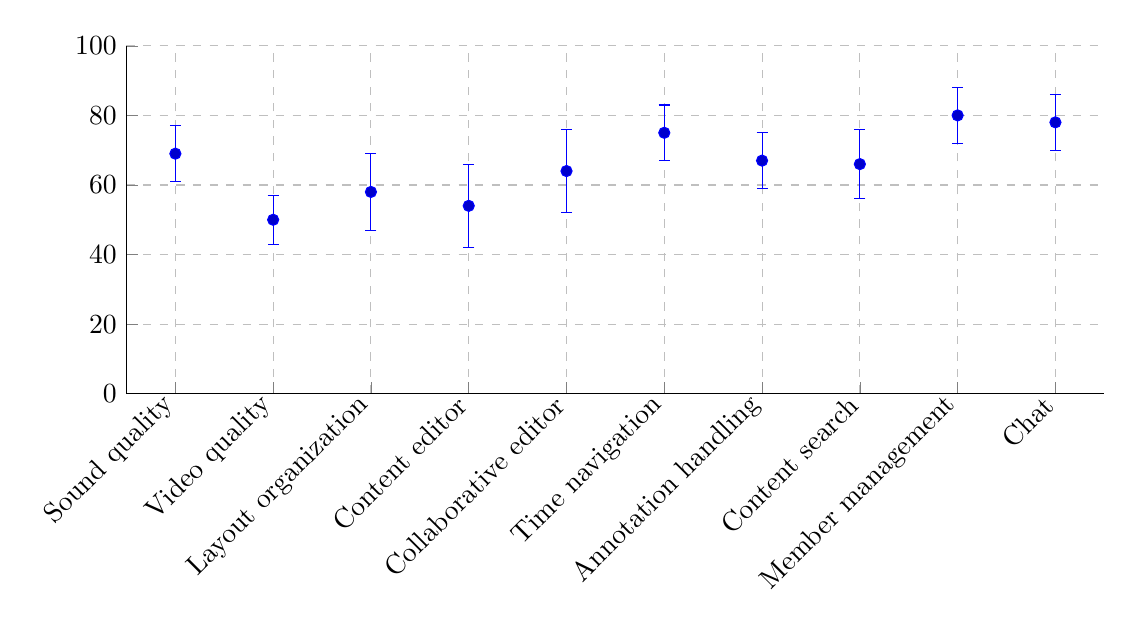
\begin{tikzpicture}[scale=1.0],
\centering
\begin{axis}[
height=6cm,
width=14cm,  
  ymax=100,
  ymin=0,
  xmin=0.5,
  xmax=10.5,
  axis y line*=left,
  axis x line*=bottom,
  xticklabels={Sound quality,Video quality,Layout organization,Content editor,Collaborative editor,Time navigation, Annotation handling, Content search,Member management,Chat},
  xtick={1,...,10},
  ytick={0,20,...,200},
      ymajorgrids=true,
      xmajorgrids=true,
      grid style=dashed,
  x tick label style={rotate=45,anchor=east}]
\addplot+[only marks][error bars/.cd,y dir=both, y explicit]
coordinates {
(1,69) +- (8,8)
(2,50) +- (7,7)
(3,58) +- (11,11)
(4,54) +- (12,12)
(5,64) +- (12,12)
(6,75) +- (8,8)
(7,67) +- (8,8)
(8,66) +- (10,10)
(9,80) +- (8,8)
(10,78) +-(8,8)
};
\addplot[dashed] coordinates {(0,0) (5.5,0)};
\end{axis}
\end{tikzpicture}%
  \end{center}
  \caption{Solution evaluation}
  \label{fig:user_evals}
\end{figure}

Most users gave us worse evaluations on our user interface layout and content editor, which was due to having a lot of tools present in the same web page and some of them were hidden due the screen size. In some cases users had to scroll down in order to find the tools they were looking for. 

Another weak aspect was our content editor, which in fact we recognize the difficulty to handle with, most due to the amount of information that is necessary to create a synchronized content (starting time, duration and content itself). Some users have suggested that the content should also be present on the time-line so they could be easily dragged and resized (on time).

We are aware that placing content on the time-line will reduce our solutions performance, especially when there is a relatively big amount of content due to the content that is present on the time-line being loaded all in once. Although, we recognize that for some cases (relatively low amount of content), displaying the content on the time-line could not have a great impact on our solutions performance. 

In conclusion, 100\% of our testers though that our solution was an innovation and 92.31\% recommended using our solution.







%\input{new_file} % add new .tex files for new chapters

\chapter{Conclusions}
\label{chapter:conclusion}

\section{Summary}
\label{section:summary}
In this thesis, our goal was the development of a web application using \emph{WebRTC} that complement current audio, text and video communications in order to create rich and collaborative interfaces with the ability to add more content on a future time. Another important goal of this project is the ability to navigate in time by rewinding communications, fast-forward and jump to certain points.

Having this in mind, we started to analyze the technologies necessary to implement our solution. In a first glance, we have analyzed the problems that real time communication applications are facing when using the current Internet infrastructure. Next we have we have analyzed the main components of the \emph{WebRTC} stack. Furthermore, we have analyzed how we could implement the signalization component that \emph{WebRTC} does not not define. Hence, with the transport component being analyzed, we have studied how we could expose content in a synchronized and interactive way. Moreover, we have performed an analysis on the kinds of media types the particularities of each one when manipulating time. Lastly, on the state of the art context, we have analyzed existing frameworks and libraries that could help us implementing a collaborative environment.

Based on our evaluation of the state of the art, we have defined the architecture of our proposed solution.

Although we have used our own signaling protocol on our implementation, the first steps we have made during the development of our prototype were using \ac{XMPP}, we have discovered the drawbacks of this approach in practice and we moved our learnings to the state of the art. Besides starting our prototype using this approach, we have used \emph{strophe.js} for performing communications with \ac{XMPP} servers. We have found and fixed a bug present on \emph{strophe.js} library that silenced an error raised by duplicated user registrations.

As a consequence of not using \ac{XMPP} for the signaling protocol, we have defined our own protocol based on \emph{WebSockets} for performing the stream between clients and \ac{KMS}. From the \ac{KMS} functionalities, our solution uses the recording feature, composite endpoints that mix multiple audio and video streams into a single one and \emph{QR code} detection for creating hyper content.

Another important contribution we have made was a bug fix of a memory leak present on \ac{KMS} which we discovered when we were doing performance tests with our solution.

\section{Achievements}
\label{section:achievements}
	We have successfully implemented the basic functionalities of our prototype and spare some time for adding more valuable features such as the ability to create content by exposing \emph{QR codes} to the camera and lastly perform changes to the user interface in order to improve the quality of user's experience.

	The performance tests that we have executed showed that our system is stable and more importantly that our web server is lightweight and most of processing power is dedicated to the streaming server.

	Our usability tests show results that are considerably worse than the established optimal values due to our solution propose a different way to communicate that most people are not used to. Although we have obtained those results, in general our users gave us positive feedback and valuable advices which we have used to improve our system. 

\section{Future Work}
\label{section:future}
	Playing back video with a faster rate is not possible using the current version of \ac{KMS} which we expect the availability of that feature in a near future but we have proposed an alternative way to implement faster playback by using \emph{ffmpeg} to convert the video before playing it.

	Although we have tested our solution in a powerful machine for the current time, our performance tests revealed that the streaming component uses a lot of resources. We left for a future work a deep analysis on the scalability of our system which we have proposed different approaches but we have not tested them.

	Another aspect we could have tested was the performance of our solution when using \ac{TURN} servers for relaying the traffic that fails using \ac{STUN}.

	Lastly, we have chosen functionality over security in respect to displaying content to users which lead to security flaws on our solution. Although we have not solved the security problems, we have proposed a solution which at the same time limits the flexibility of adding new functionalities to our prototype.
\cleardoublepage
 % file "Thesis_Conclusions.tex"

% ----------------------------------------------------------------------
%  TODO - Appendix (optional)
% ----------------------------------------------------------------------
\appendix
\chapter{Vector calculus}
\label{chapter:appendix}

Use to include images/diagrams tables which are important but were to big to include in the main tex.

Note that in no case the document can exceed a total of 100 pages.

Some equations examples:

\section{Vector identities}
\label{section:vectorIdentities}

\begin{equation}
	\nabla \times \left( \nabla \phi \right) = 0
	\label{eq:cross_nnp}
\end{equation}

\begin{equation}
	\nabla \cdot \left( \nabla \times {\bf u} \right) = 0
	\label{eq:dotCross_nnu}
\end{equation}

\cleardoublepage

 % file "Thesis_Appendix.tex"

% ----------------------------------------------------------------------
%  Bibliography
% ----------------------------------------------------------------------


% External bibliography database file in the BibTeX format
\cleardoublepage

\bibliographystyle{splncs}
% TODO - This file "references.bib" should include all your bibtex
\bibliography{references} 

% Add entry in the table of contents as chapter
\addcontentsline{toc}{chapter}{\bibname}
\cleardoublepage

\end{document}

\printbibliography
\end{document}

\grid
\grid
